\chapter{MapAlign: Training and Model Approaches}

This chapter provides a detailed and comprehensive analysis of the developed architecture throughout its various phases, focusing particularly on the two approaches that reached the most promising results.

\section{Feature-Based Localization}

The first approach developed relied on features already extracted by neural networks running on the car during its operations. These networks captured details like curbs, road markings, and boundaries from image sequences, and the extracted features were saved in a compact data format. By using this pre-processed information instead of raw images, the model significantly reduced the size of the input data.

The developed architecture consists of four main components: the preprocessor, backbone, decoder, and network head. Each of these components is analyzed in detail.

The \textit{BEVPreprocessor} prepares the input data with a simple structure consisting of a single convolutional layer with just $0.0013$ million parameters, keeping it efficient. This ensures that all input data is resized to the same dimensions, allowing it to be combined into a single tensor for improved representation.

The \textit{Backbone}, built on the BiSeNetV1 architecture \cite{DBLP:journals/corr/abs-1808-00897}, is the most complex component, containing $12.63$ million parameters. Its main role is to extract relevant features while discarding unnecessary data. As illustrated in Figure~\ref{fig:bisenetv1}, the backbone operates using two distinct paths:
\begin{enumerate}
    \item Spatial Path: Designed with a small stride to preserve spatial details, this path captures high-resolution features through several convolutional layers, emphasizing fine-grained spatial information.
    \item Context Path: This path quickly down-samples the input to expand the receptive field, helping the model capture broader context. It utilizes Attention Refinement Modules (ARMs) and additional convolutional layers. ARMs allow the model to focus on important regions within the input tensor, significantly contributing to the model's parameter count.
\end{enumerate}
\begin{figure}[H]
    \centering
    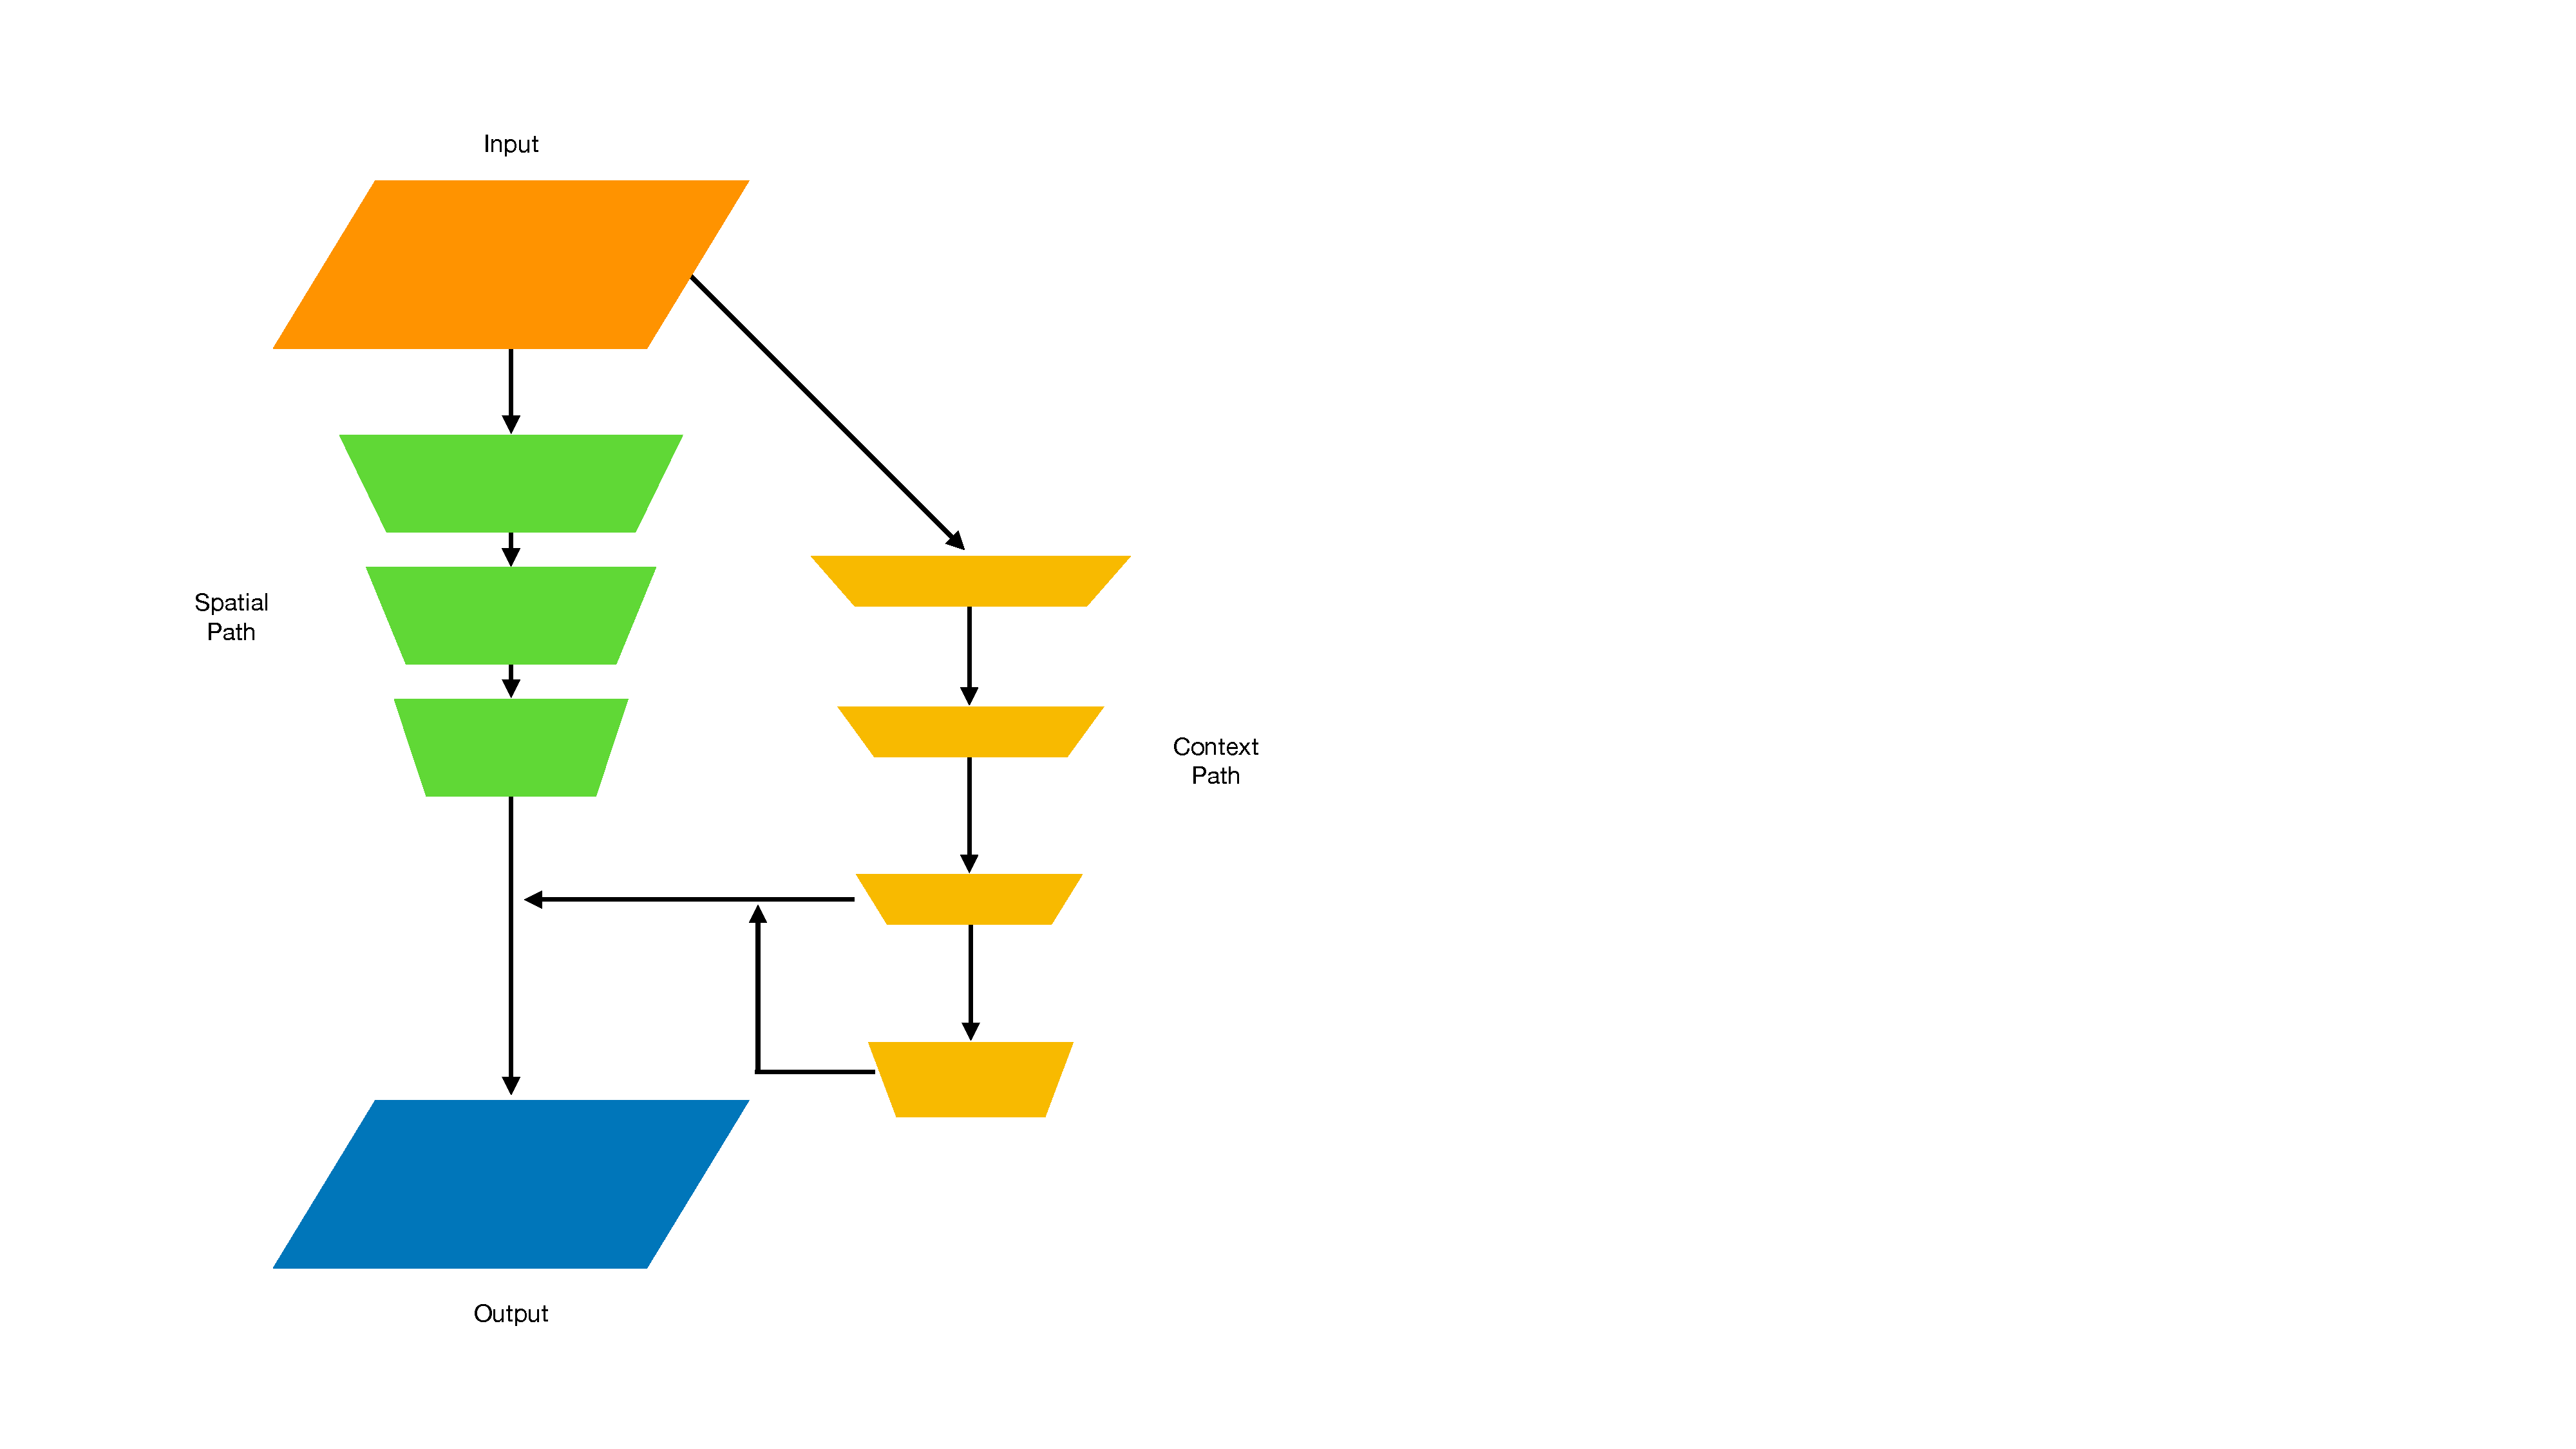
\includegraphics[width=0.5\linewidth]{LateX//figs/bisenetv1.pdf}
    \caption{Architecture of BiSeNetV1 Backbone. The backbone comprises two parallel paths: the Spatial Path and the Context Path. The dual-path structure enables efficient and accurate segmentation by combining spatial information with global context.}
    \label{fig:bisenetv1}
\end{figure}
A Feature Fusion Module is then used to efficiently combine the features from the Spatial and Context Paths.

The \textit{Decoder} then up-samples these features to restore them to the original input resolution, with a parameter count of $0.0924$ million. The role of the decoder is to convert high-level, low-resolution features back into the detailed, high-resolution format needed for accurate output. This component ensures that the model’s outputs match the input tensor's scale, making the model suitable for precise localization tasks.

The head, generates the segmentation output, while a fully connected (Fc) layer finalizes the pose estimation. This design enables efficient and accurate pose analysis. The model’s total parameter count is optimized to balance processing efficiency and accuracy.

Figure~\ref{fig:model1} illustrates the complete structure of the proposed model. The diagram provides a detailed overview of the architecture, showcasing the various components and their interactions. 
\begin{figure}[H]
    \centering
    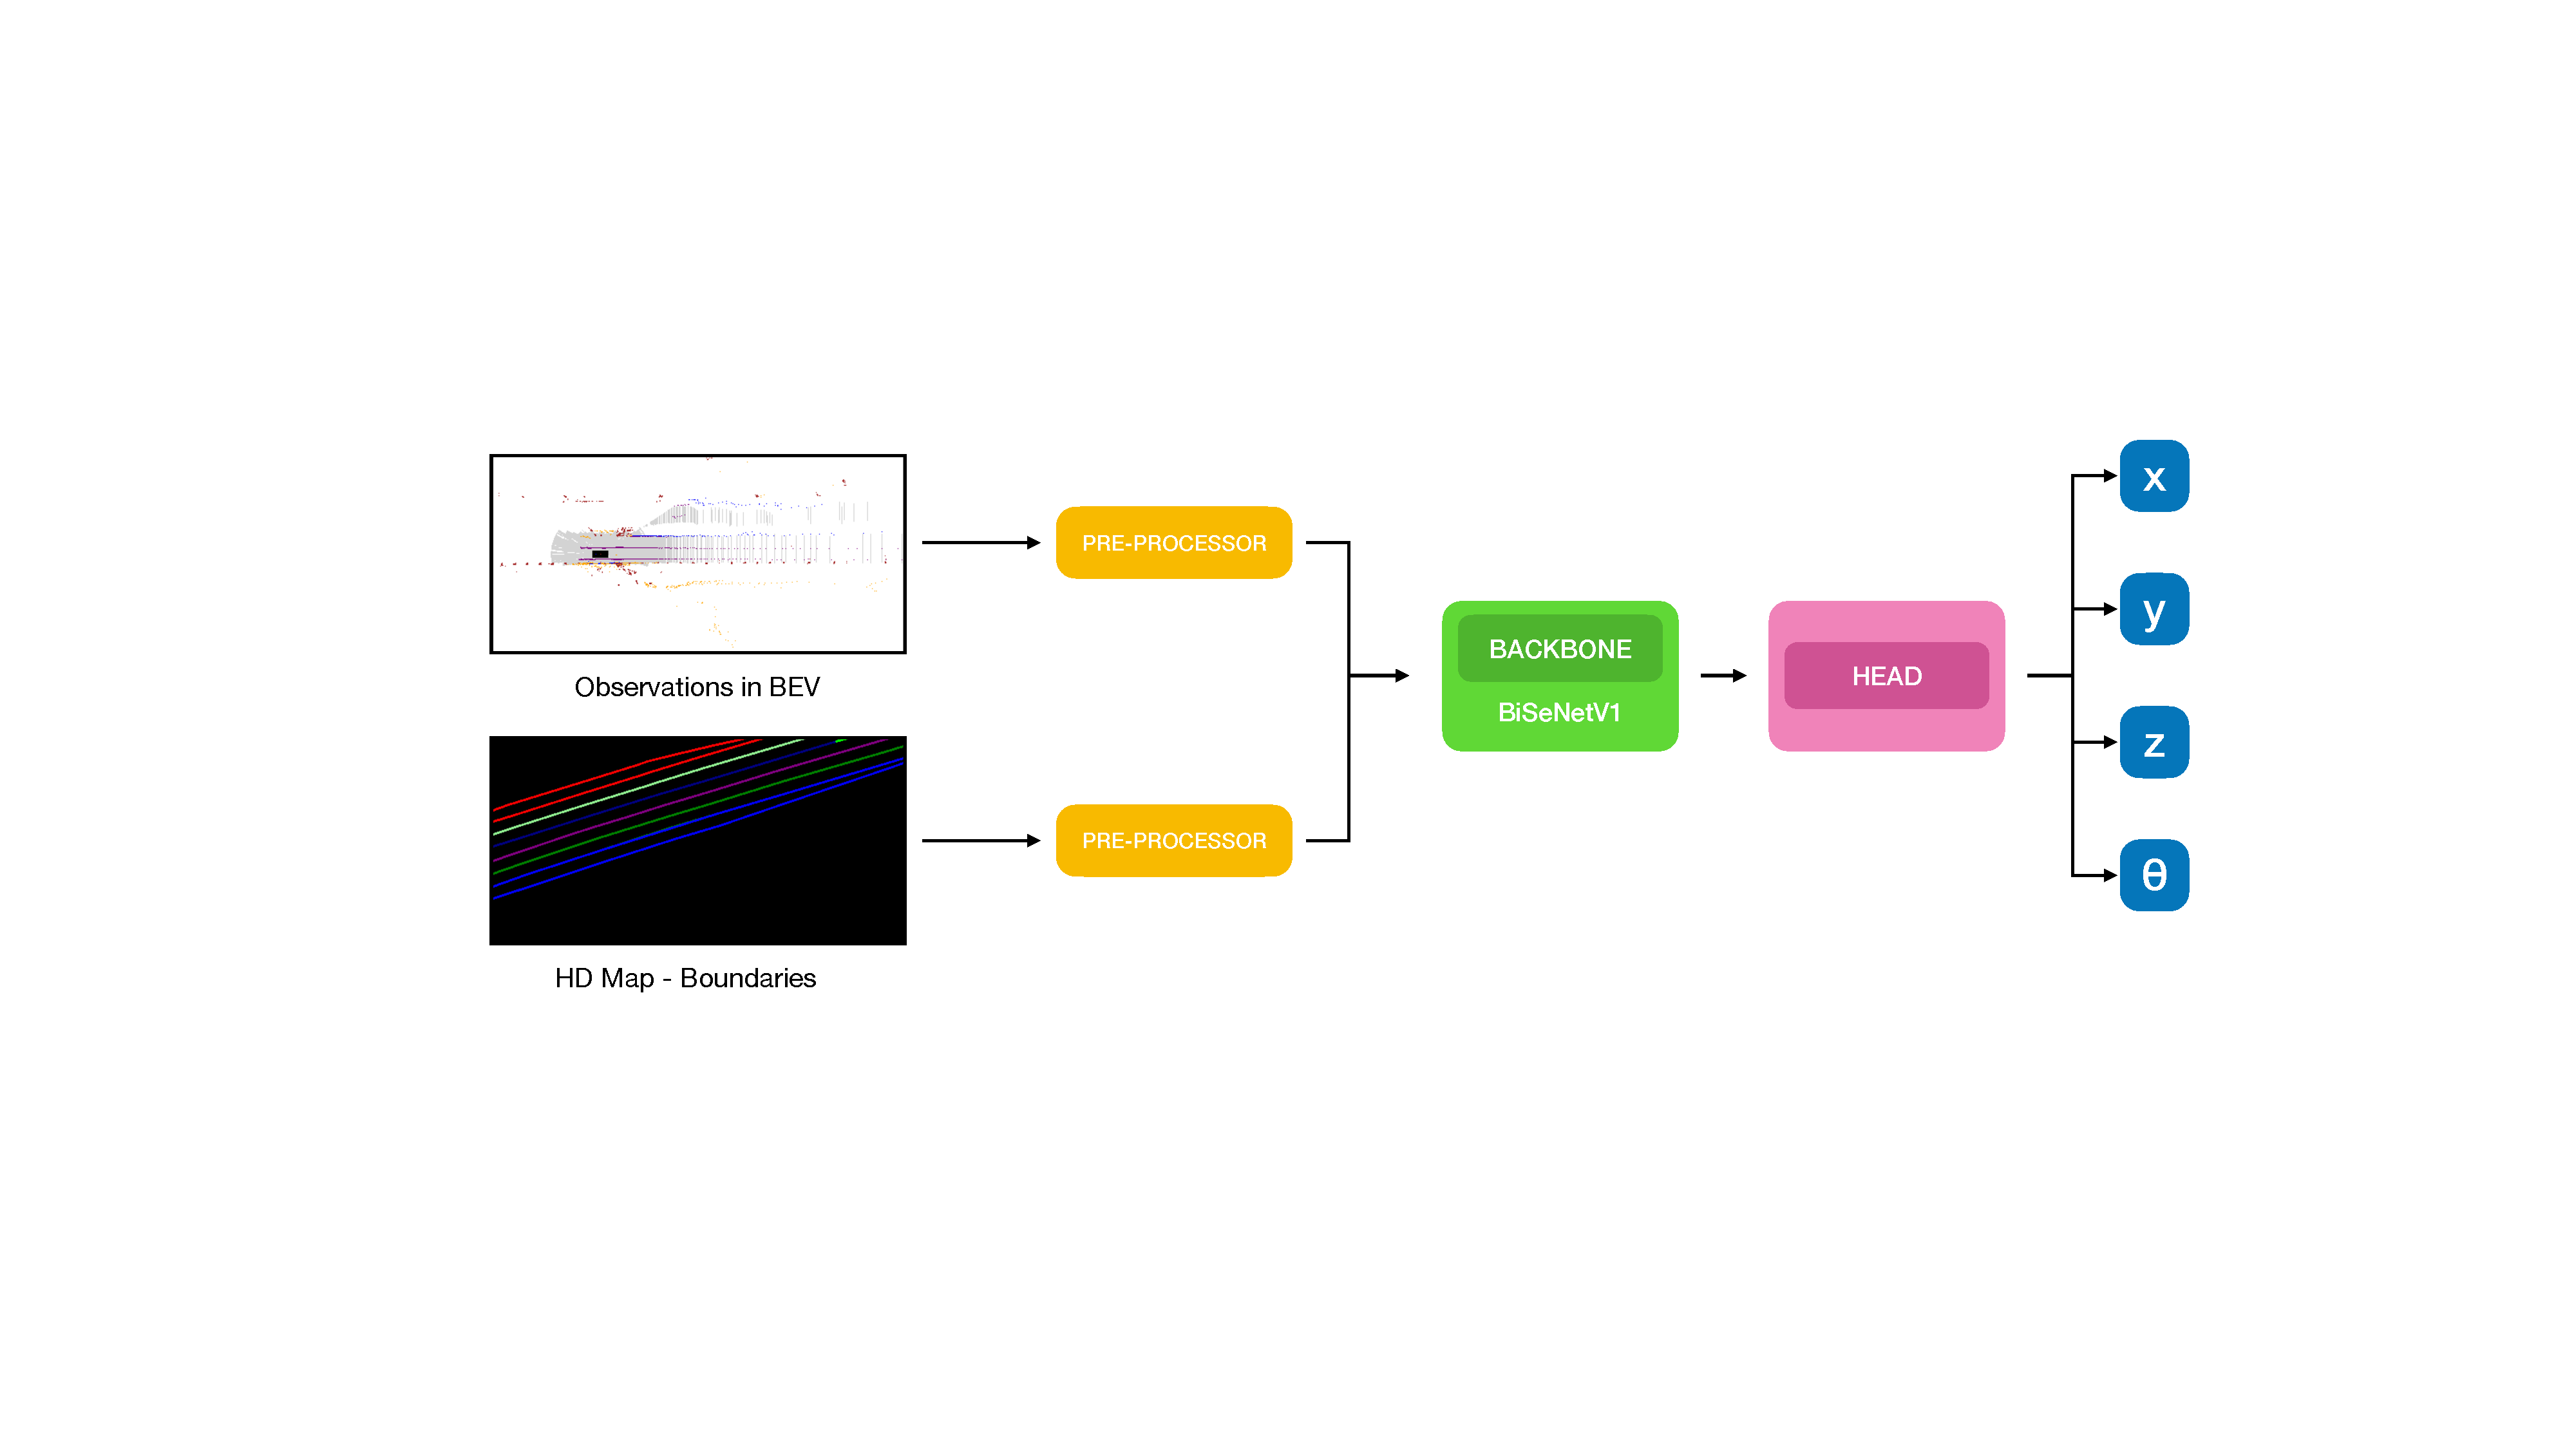
\includegraphics[width=1\linewidth]{LateX//figs/architecture1.pdf}
    \caption{Overview of the complete model architecture, illustrating input processing, feature extraction, and output generation.}
    \label{fig:model1}
\end{figure}

The primary goal of this model was to accurately predict the four values that allow the alignment between the car pose and the HD map: translations along the \( x, y, z \) axes and the heading angle. Alongside model design, appropriate loss functions were also defined. As described in Chapter 1, the three loss functions used were L1, L1-smooth, and MSE.
It is advantageous to employ a single loss function that accounts for all parameters collectively, as this ensures the network learns to optimize the relationships and trade-offs between them in a comprehensive manner. However, incorporating individual loss components for each parameter can further enhance the model's performance by encouraging it to focus on specific prediction tasks. This approach enhances interpretability by enabling the network to recognize parameter-specific shades and promotes generalization by preventing any single parameter from dominating the optimization process. For this reason two additional specialized losses for the translationvalues and heading angle were added. 
The heading angle was especially critical and challenging to learn accurately, so this structure was consistent across different model versions.

The initial iterations used the following high-level parameters:
\begin{itemize}
    \item Data augmentation: Included body rotations between $-30^\circ$ and $30^\circ$, and horizontal and vertical shifts up to $10\%$;
    \item Optimizer: Training used the SGD optimizer with a base learning rate of \textit{0.1} and a batch size of \textit{64};
    \item Learning Rate Scheduler: The scheduler was WarmupPolyLR \cite{kalra2024warmuplearningrateunderlying} with a warm-up period of $5000$ iterations, capped at a maximum of $100000$ iterations;
    \item Automatic Mixed Precision (AMP) was enabled to improve training speed and resource use.
\end{itemize}

The learning rate was selected to achieve the following behavior during training:
\begin{figure}[H]
    \centering
    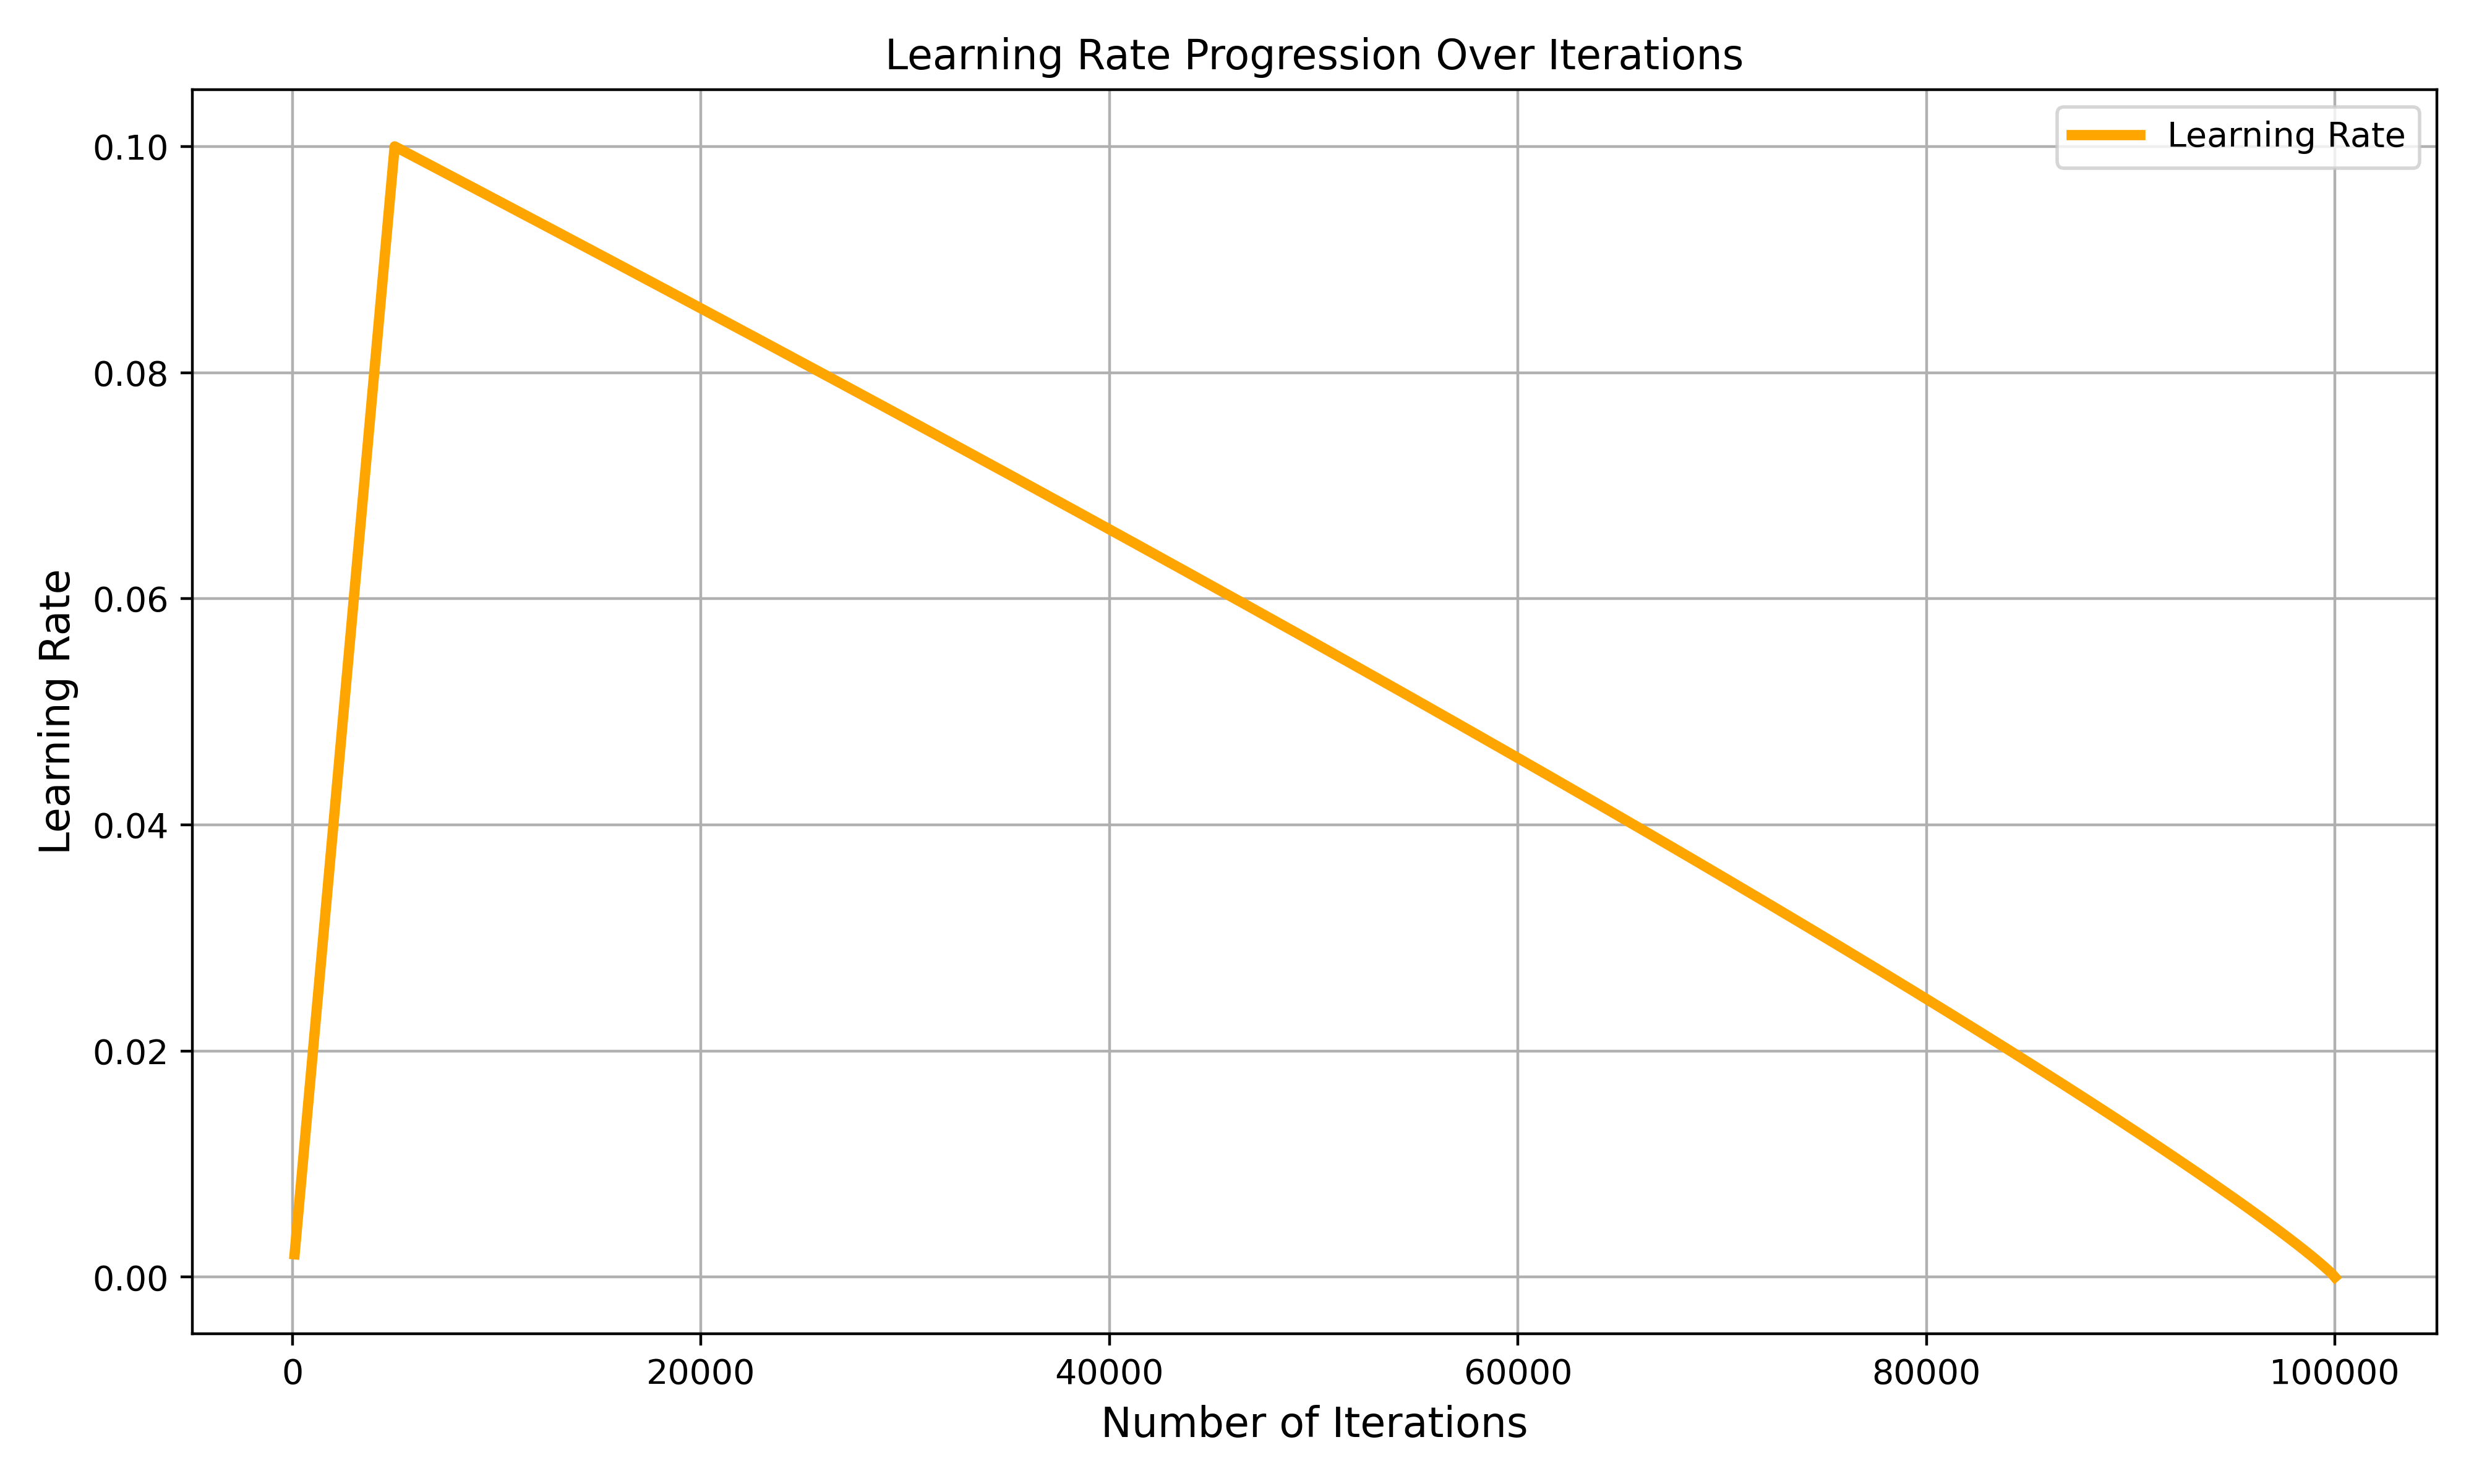
\includegraphics[width=0.75\linewidth]{LateX//figs/learning_rate_progression.png}
    \caption{Learning rate progression during training, showcasing an initial warm-up phase followed by a gradual decrease. The learning rate peaks at a maximum value of 0.1 at 5000 iterations.}
    \label{fig:learning-rate-progression}
\end{figure}

Checkpoints were saved every $100$ iterations, and evaluations were performed every $5000$ iterations using the \textit{PoseEvaluator}. The evaluator calculated the L1 loss on a validation set to objectively assess the model’s performance. The evaluation values were computed as the absolute difference between the ground truth and predicted values for position and heading, as shown below:
\begin{align}
    \text{eval}_x &= |x_{\text{gt}} - x_{\text{pred}}|, \\
    \text{eval}_y &= |y_{\text{gt}} - y_{\text{pred}}|, \\
    \text{eval}_z &= |z_{\text{gt}} - z_{\text{pred}}|, \\
    \text{eval}_{\theta} &= |\theta_{\text{gt}} - \theta_{\text{pred}}|.
\end{align}
Since the z-axis is not augmented, the ground truth for translation along this axis must always be zero. Consequently, the network is required to consistently output always the same value.

Training was accelerated with CUDA, using CuDNN benchmarking for improved speed. Initial training sessions utilized only a portion of the dataset to refine the model’s structure and functionality before scaling to the full dataset. The used dataset focused on sequences captured in the southern part of the city. 

\subsection*{Minor Dataset Split with Heading Angle in Radians}
\subsubsection*{MSE}
The first training session of the architecture described used MSE as Loss function, along with the parameters described above. This approach resulted in a regular decreasing loss, as shown in Figure~\ref{fig:mse-loss-progression}:
\begin{figure}[H]
    \centering
    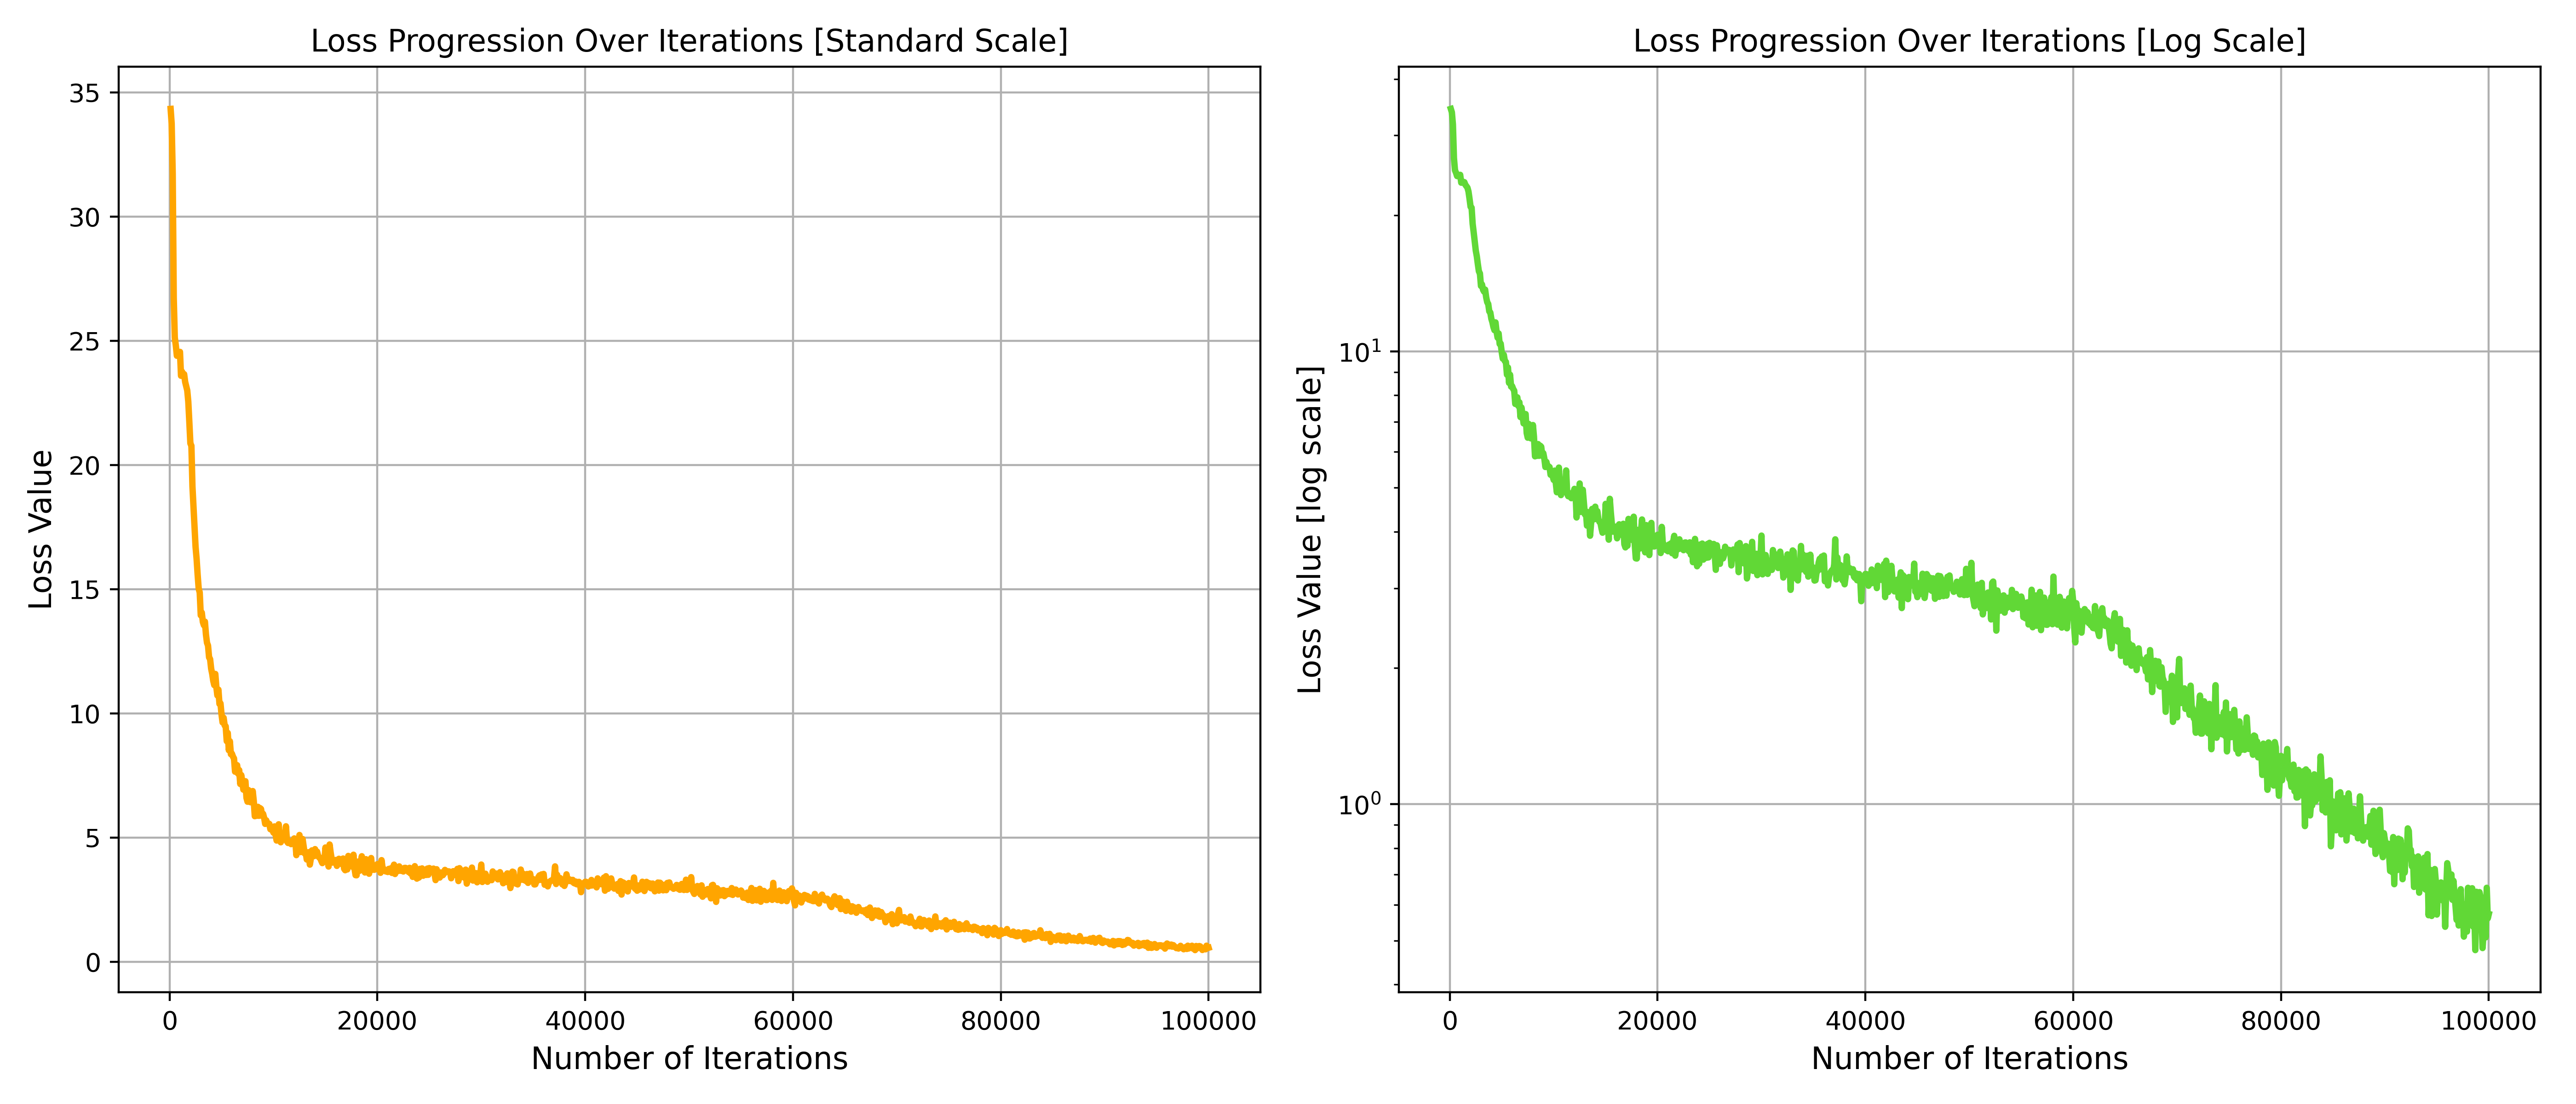
\includegraphics[width=1\linewidth]{LateX//figs/loss_total_mse_progression_comparison.png}
    \caption{Total loss progression using the Mean Squared Error (MSE) as the loss function. The plot includes a standard scale on the left and a logarithmic scale on the right for an improved visualization.}
    \label{fig:mse-loss-progression}
\end{figure}

Focusing on specific losses for pose and heading angle, the following pattern was observed:
\begin{figure}[H]
    \centering
    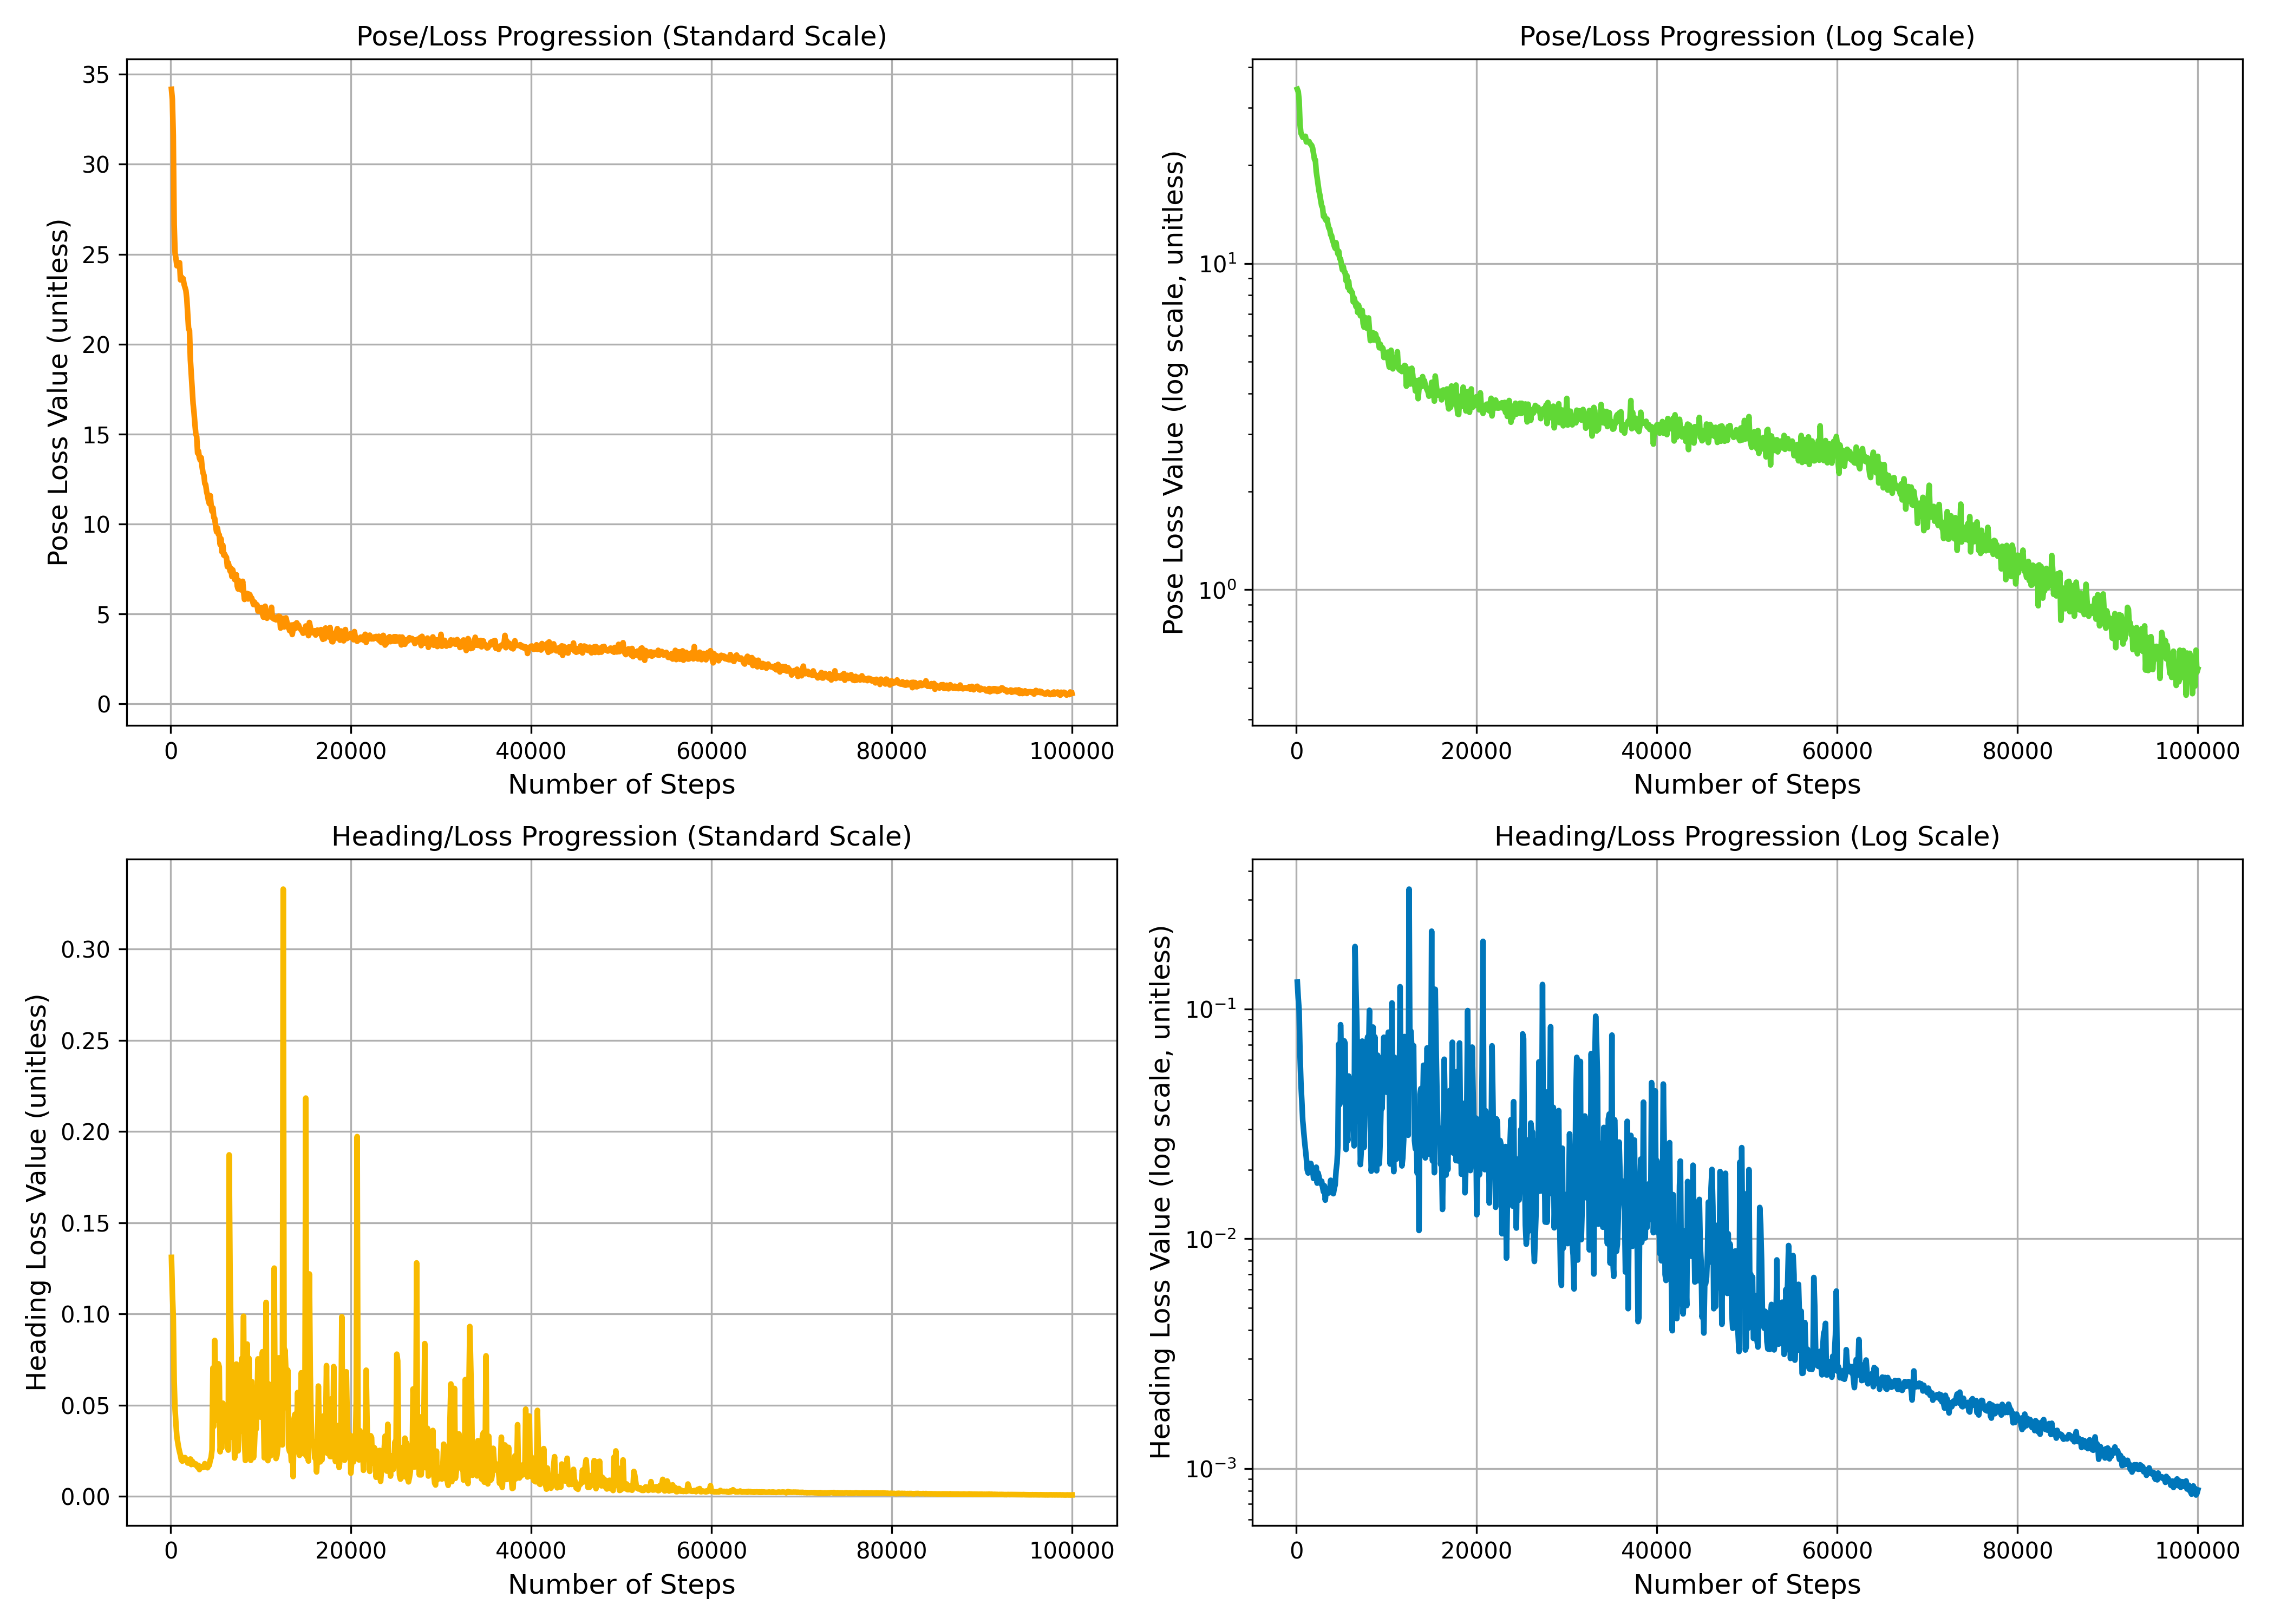
\includegraphics[width=1\linewidth]{LateX//figs/mse_pose_heading_loss_comparison.png}
    \caption{Pose (orange) and Heading (yellow) Loss comparison during training. The plot includes a standard scale on the left and a logarithmic scale on the right.}
    \label{fig:pose-heading-loss}
\end{figure}

The model's performances during evaluation aligned with expectations, and the training evaluations yielded the results that are reported in Table~\ref{tab:pose_variations_mse}:
\begin{table}[H]
    \centering
    \scriptsize
    \renewcommand{\arraystretch}{1.2} 
    \setlength{\tabcolsep}{10pt}
    \begin{tabular}{c c c c c}
        \toprule
        \textbf{Iteration} & \textbf{$\Delta$ Pose [m]} & \textbf{$\Delta \theta$ [rad] $\rightarrow$ [deg]} & \textbf{$\Delta x + \Delta y$ [m]} & \textbf{$\Delta h$ [m]} \\
        \midrule
        \num{20000}  & 2.02 & $0.05 \rightarrow 2.86$  & 1.94 & 0.08 \\
        \num{40000}  & 1.43 & $0.22 \rightarrow 12.6$  & 1.37 & 0.06 \\
        \num{60000}  & 1.42 & $0.04 \rightarrow 2.29$  & 1.39 & 0.02 \\
        \num{80000}  & 1.99 & $0.02 \rightarrow 1.15$  & 1.99 & 0.00 \\
        \num{100000} & 1.54 & $0.02 \rightarrow 1.15$  & 1.54 & 0.00 \\
        \bottomrule
    \end{tabular}
    \caption{Evaluation (L1) values in pose, angle, combined displacement ($\Delta x + \Delta y$), and height across iterations using MSE Loss Function.}
    \label{tab:pose_variations_mse}
\end{table}

Despite the loss functions decreasing and reaching very low values, indicating potential generalization and effective learning, the evaluation process reveals that the results are still not optimal or acceptable. The positional error exceeds one meter, which is insufficient for HD map alignment applications, as discussed in Chapter 1. This could be acceptable if iterative optimization was still included in the desired pipeline of the dataset generator. This approach could simply eliminate the part where the sequences had to be manually aligned. However, it was not sufficient, so other attempts were made and will be further demonstrated. 

\subsubsection*{L1 Loss}
The results with the L1 loss are consistent with previous observations. 
Figure ~\ref{fig:network-training-results1} illustrates the behavior of the neural network. Vertically, the first three images represent the inputs: features extracted directly by the car, associated HD maps, and the fusion of the two. The fourth image represents the target, which is the perfect alignment that the network aims to achieve. The final image shows the network's prediction. This time, the prediction has been post-processed to apply a roto-translation of the car and its reconstructed environment.

The results, illustrated in Figure~\ref{fig:network-training-results1}, show measurements taken at two stages of training: one at the start and one near the end. Initially, the network produces inaccurate values, as it has not yet learned to generalize effectively. This is evident from the misalignment between the map and the car's reconstructed environment. By the end of training, as shown in the image on the right, the network's performance improves significantly, reducing the misalignments, though they are not completely overcame.
\begin{figure}[H]
    \centering
    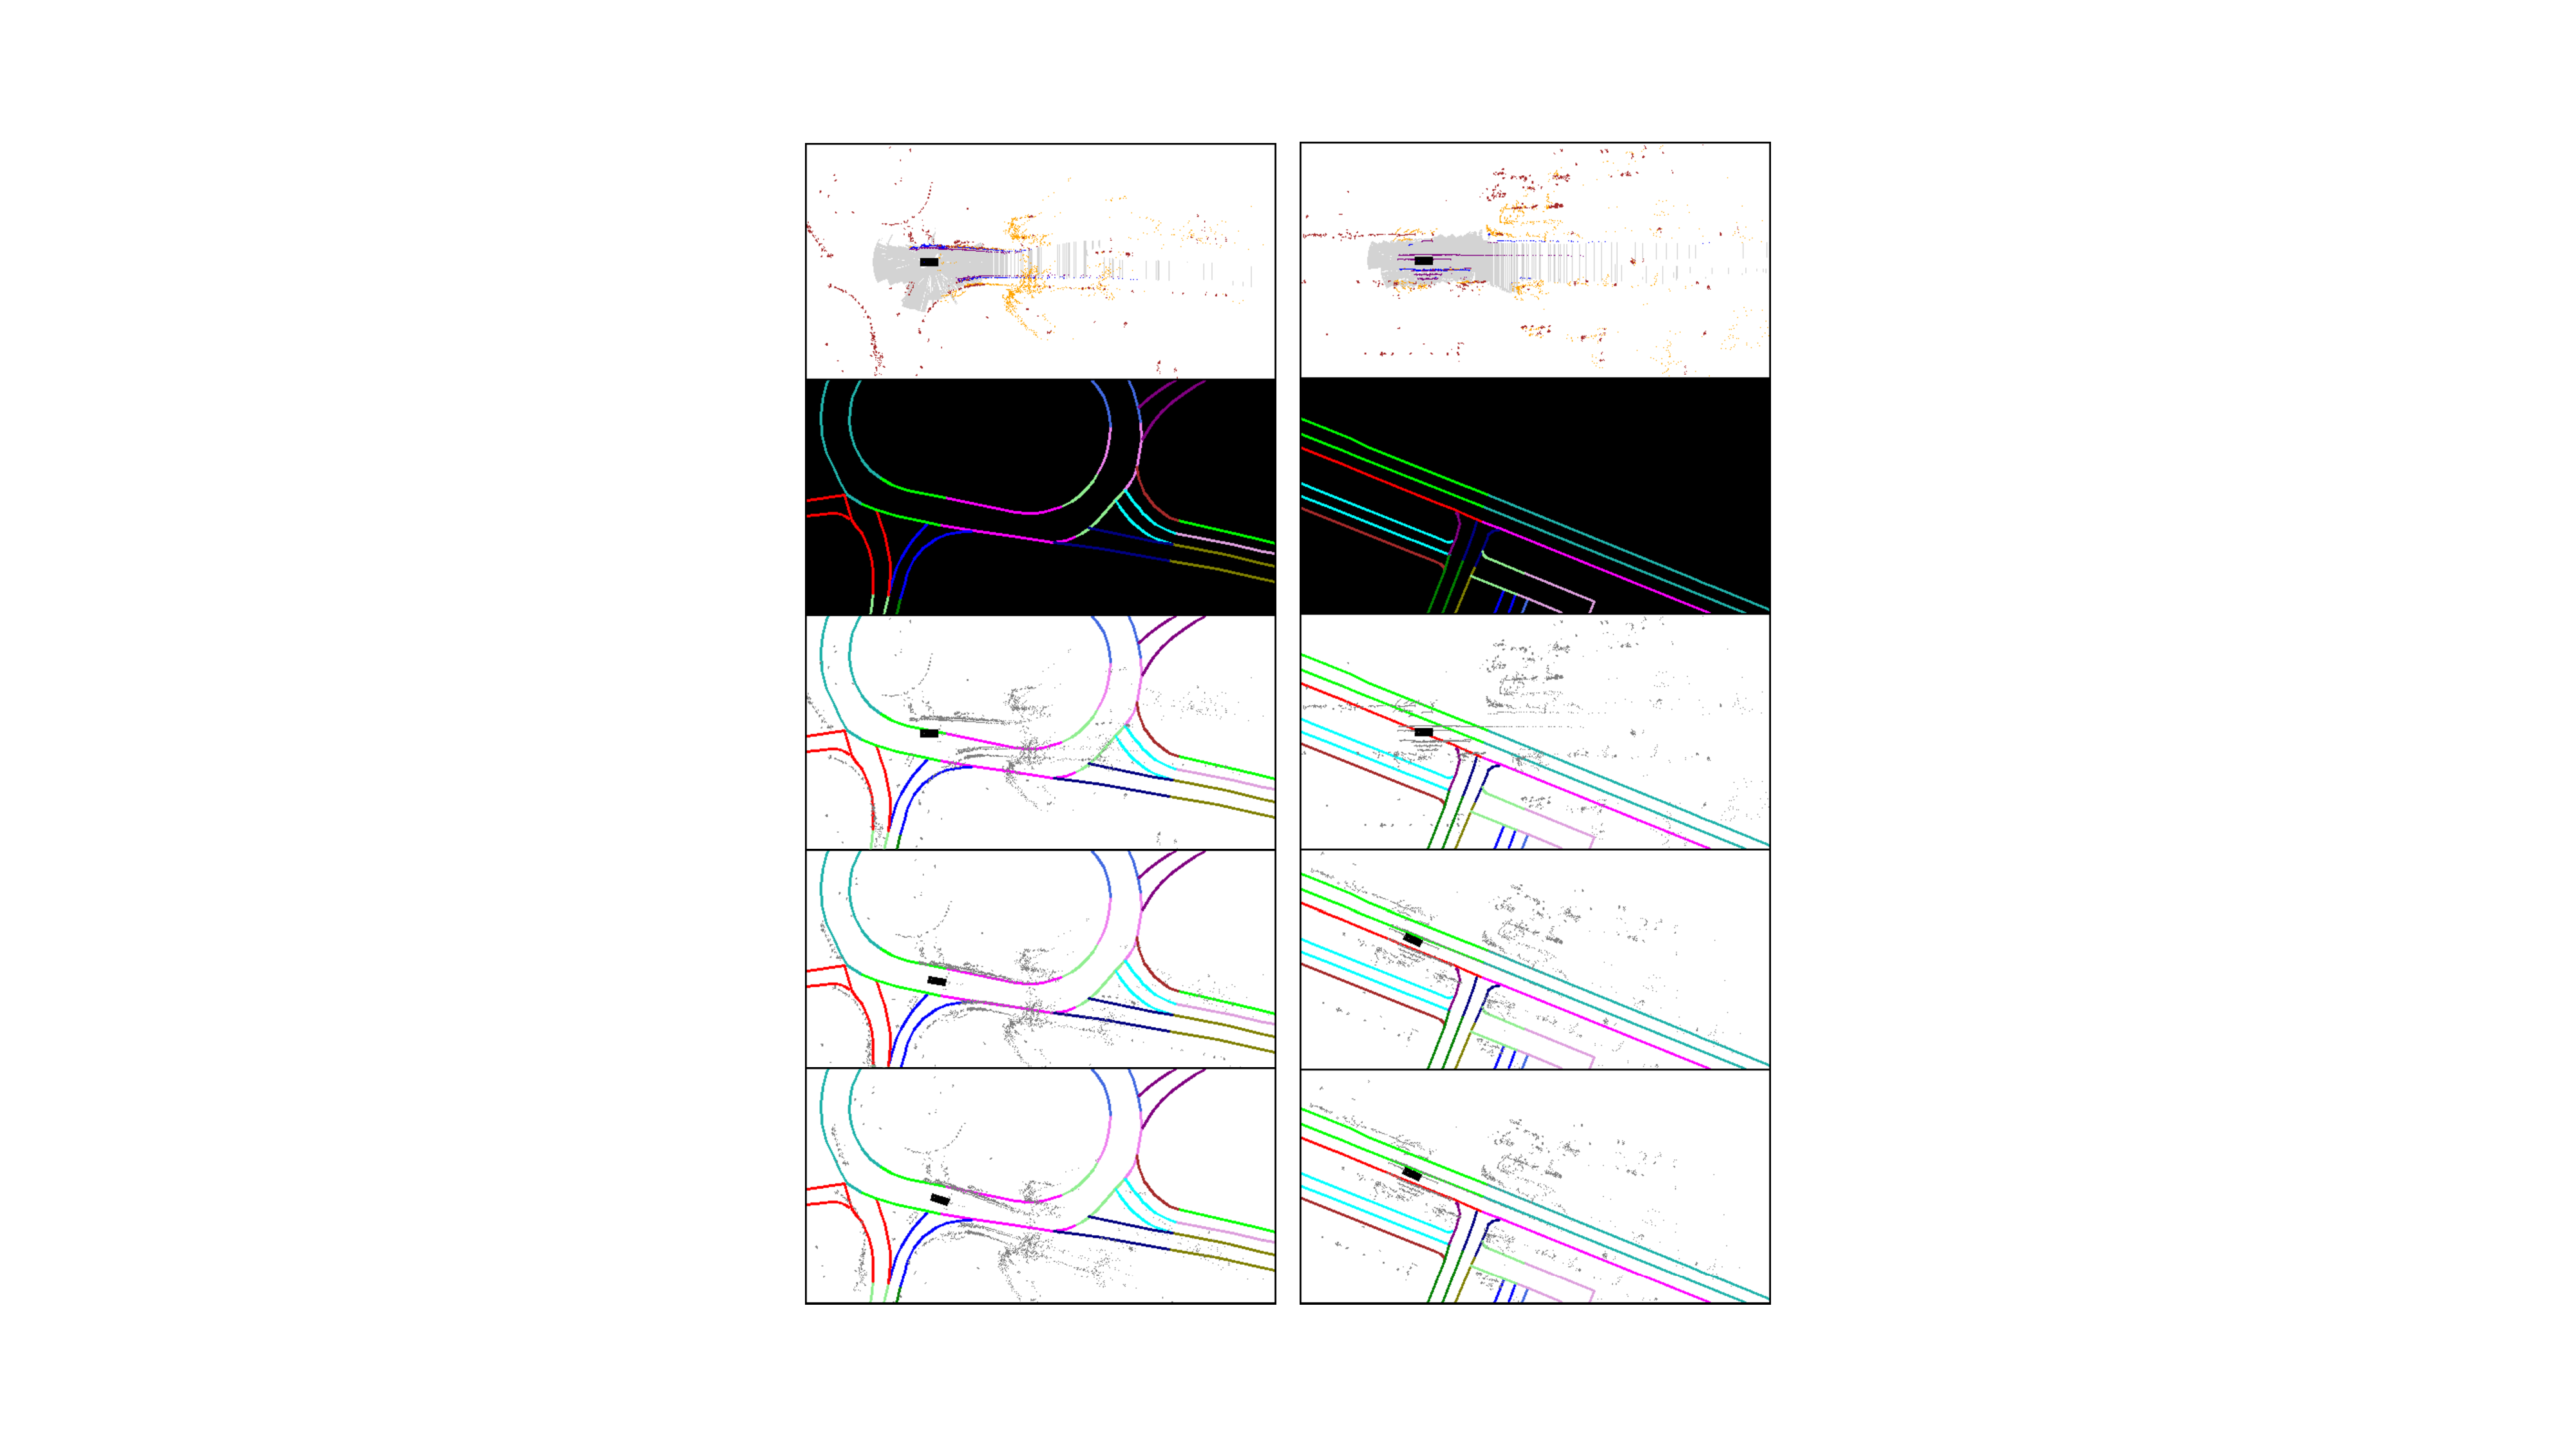
\includegraphics[width=1\linewidth]{LateX//figs/IMMAGINI_L1_rete.pdf}
    \caption{Network performance at the beginning (left) and at the end (right) of training, showing improved alignment and reduced errors.}
    \label{fig:network-training-results1}
\end{figure}

Since the specific loss graphs didn’t show any significant difference, only the evaluation Table is presented for this experiment.
\begin{table}[H]
    \centering
    \scriptsize
    \renewcommand{\arraystretch}{1.2} 
    \setlength{\tabcolsep}{10pt} 
    \begin{tabular}{c c c c c}
        \toprule
        \textbf{Iteration} & \textbf{$\Delta$ Pose [m]} & \textbf{$\Delta \theta$ [rad] $\rightarrow$ [deg]} & \textbf{$\Delta x + \Delta y$ [m]} & \textbf{$\Delta h$ [m]} \\
        \midrule
        \num{20000}  & 2.00 & $0.11 \rightarrow 6.31$  & 1.98 & 0.02 \\
        \num{40000}  & 1.89 & $0.13 \rightarrow 7.45$  & 1.84 & 0.05 \\
        \num{60000}  & 1.45 & $0.04 \rightarrow 2.29$  & 1.43 & 0.02 \\
        \num{80000}  & 1.42 & $0.04 \rightarrow 2.29$  & 1.40 & 0.02 \\
        \num{100000} & 1.40 & $0.03 \rightarrow 1.72$  & 1.40 & 0.00 \\
        \bottomrule
    \end{tabular}
    \caption{Evaluation (L1) values in pose, angle, combined displacement ($\Delta x + \Delta y$), and height across iterations using L1 Loss Function.}
    \label{tab:pose_variations_l1}
\end{table}
On the small test set, it is clear that simply switching the loss function to L1 is not enough to achieve the desired precision which is required to eliminate the iterative optimizer.

\subsubsection*{Smooth L1 Loss}
In this other experiment, the Smooth L1 loss, which is similar to L1 but less sensitive to outliers, was employed. The training results, as expected, remained consistent. However, this time, some interesting differences emerged. The results demonstrated slight improvements compared to previous attempts. Both loss graphs and the evaluation Table are provided below to illustrate the pattern.

The total loss graph shows the expected trend, as illustrated in Figure ~\ref{fig:smooth-l1-total-loss}, with a gradual decrease as the number of iterations increases.
\begin{figure}[H]
    \centering
    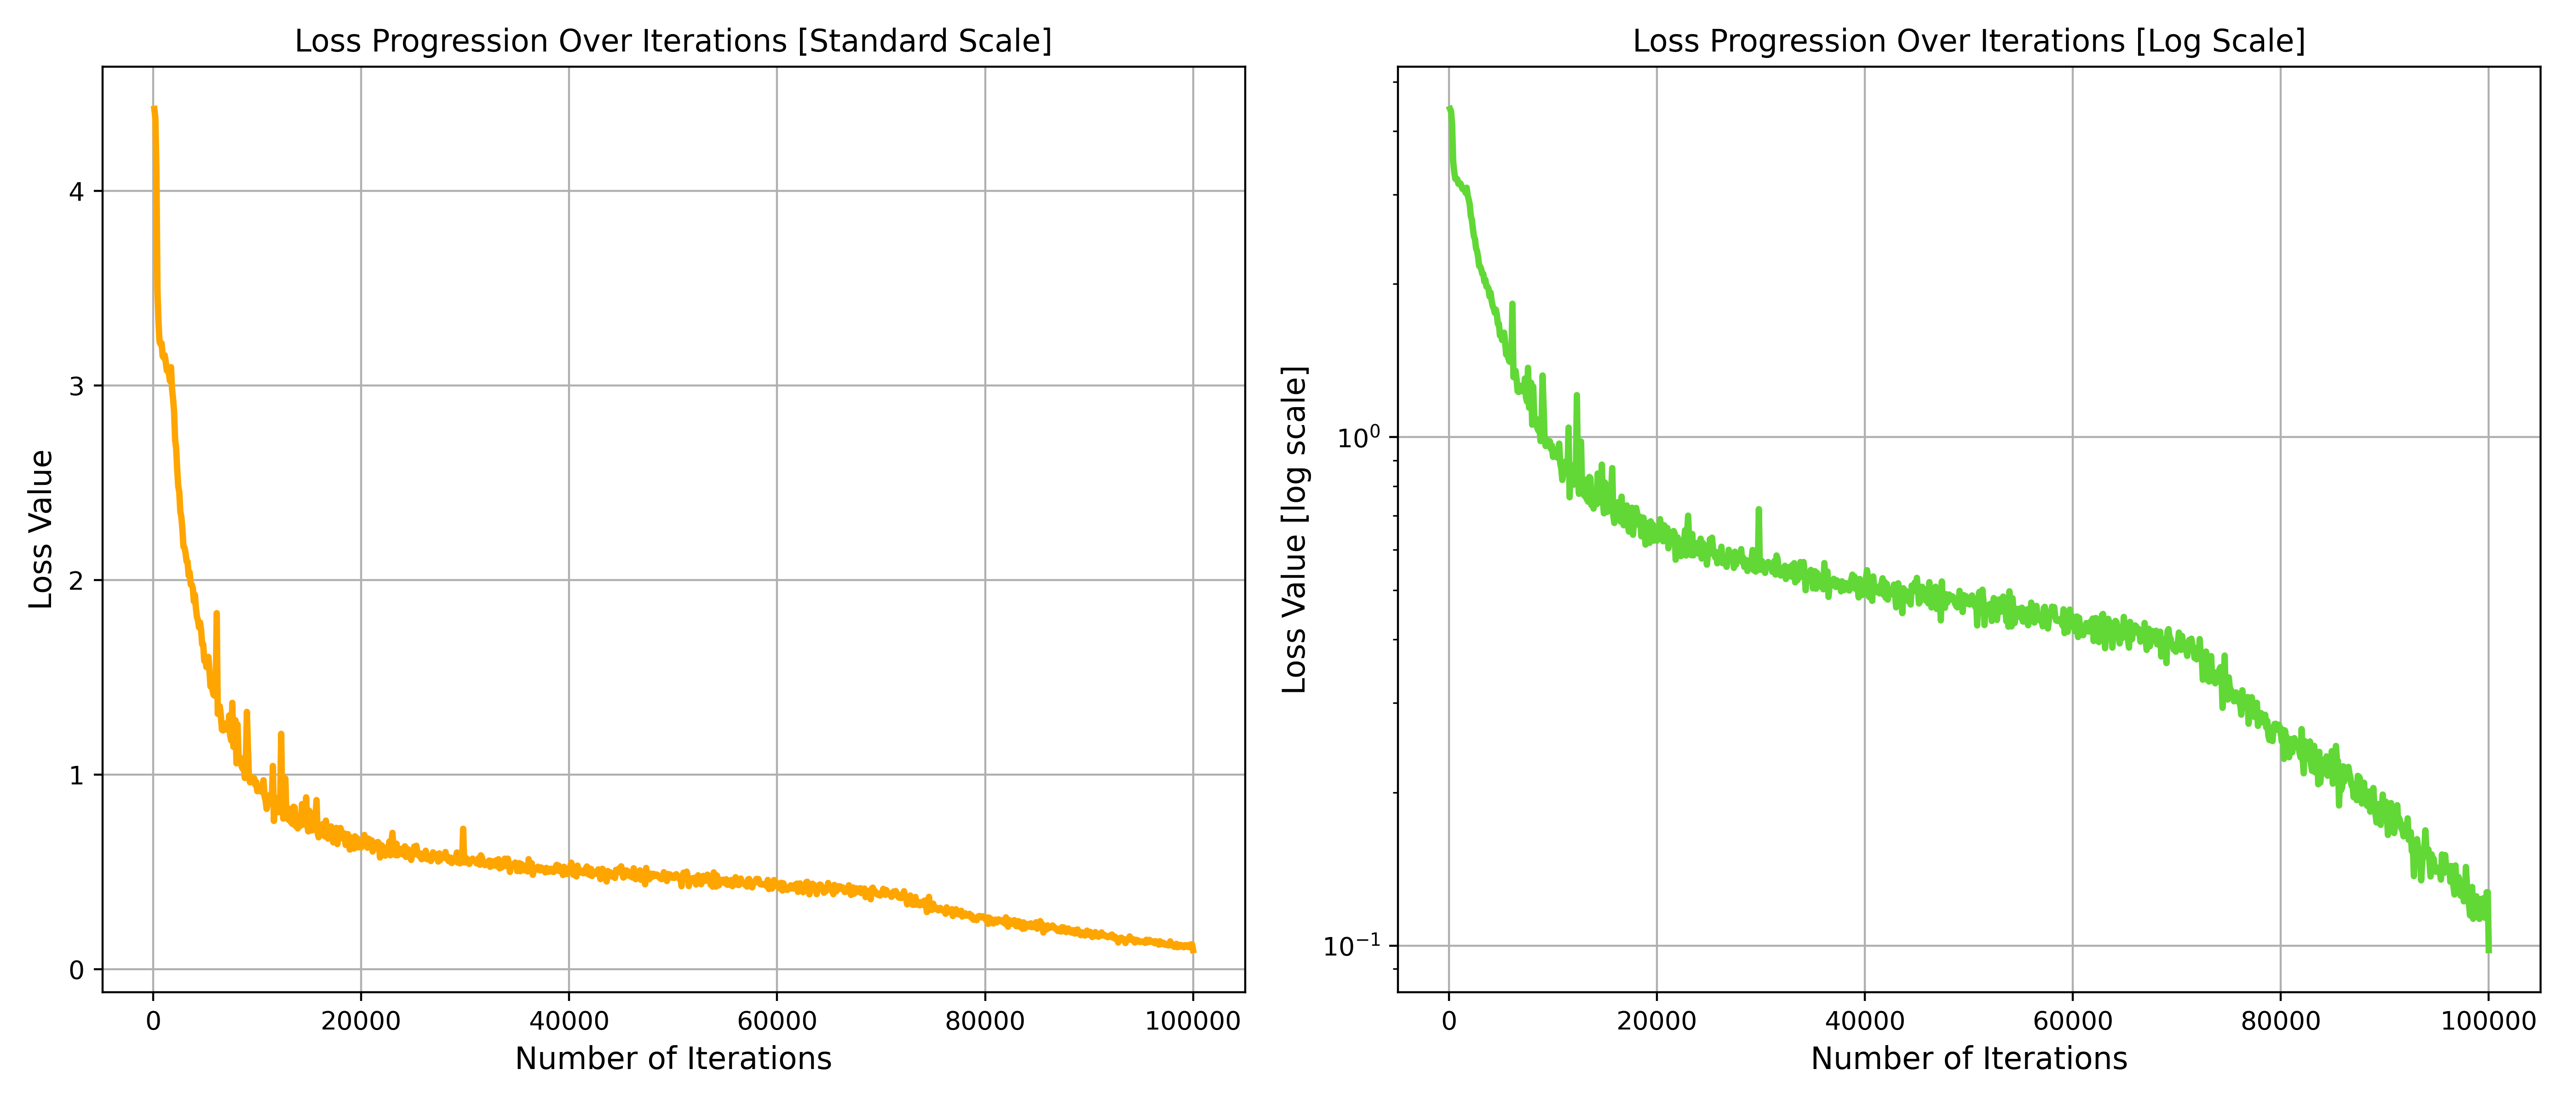
\includegraphics[width=0.95\linewidth]{LateX//figs/loss_total_l1s_progression_comparison.png}
    \caption{Total loss progression using Smooth L1 as Loss function. The plot includes a standard scale on the left and a logarithmic scale on the right.}
    \label{fig:smooth-l1-total-loss}
\end{figure}

As shown in Figure~\ref{fig:smooth-l1-pose-heading-loss}, the total Loss contributions reveal that the translation component constitutes the majority, while the heading loss contributes only a minor portion to the overall result. This observation prompted further investigation into this behavior in following experiments.
\begin{figure}[H]
    \centering
    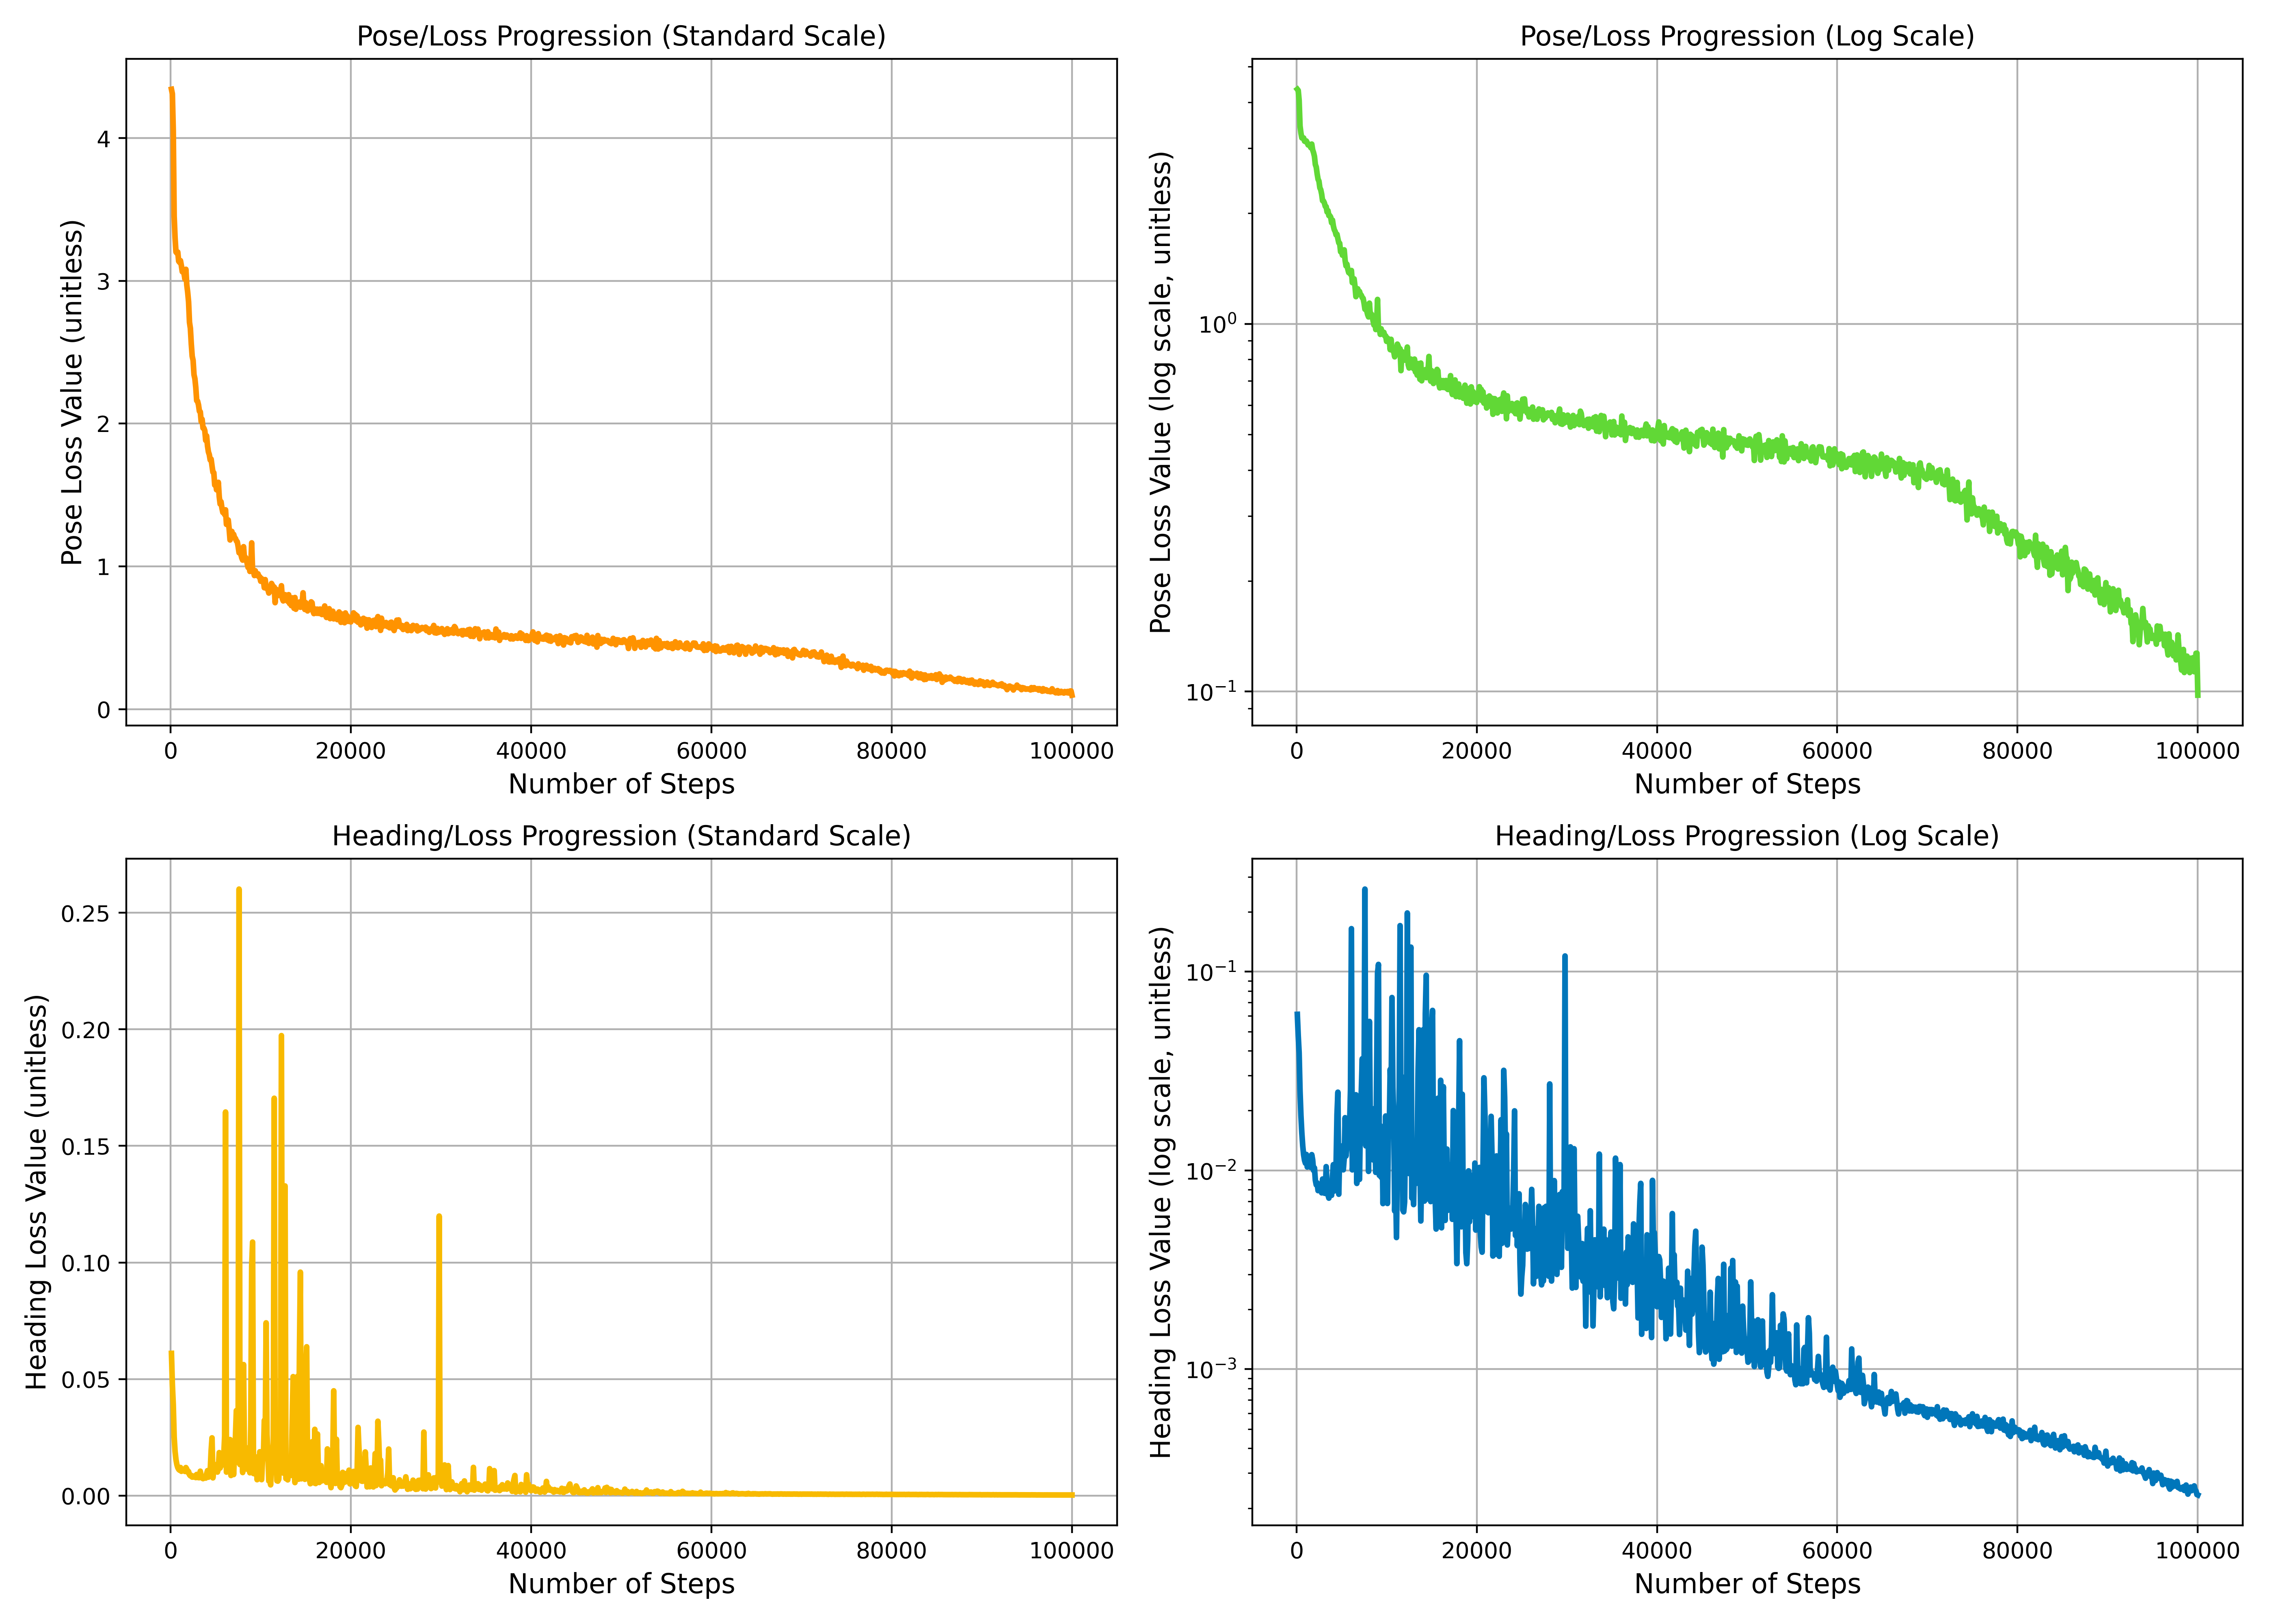
\includegraphics[width=0.95\linewidth]{LateX//figs/l1s_pose_heading_loss_comparison.png}
    \caption{Pose (orange) and Heading (yellow) Loss comparison during training. The plot includes a standard scale on the left and a logarithmic scale on the right.}
    \label{fig:smooth-l1-pose-heading-loss}
\end{figure}

Below is reported a summary of the evaluation results observed during the training session:
\begin{table}[H]
    \centering
    \scriptsize
    \renewcommand{\arraystretch}{1.2} 
    \setlength{\tabcolsep}{10pt} 
    \begin{tabular}{c c c c c}
        \toprule
        \textbf{Iteration} & \textbf{$\Delta$ Pose [m]} & \textbf{$\Delta \theta$ [rad] $\rightarrow$ [deg]} & \textbf{$\Delta x + \Delta y$ [m]} & \textbf{$\Delta h$ [m]} \\
        \midrule
        \num{20000}  & 1.75 & $0.14 \rightarrow 8.02$  & 1.73 & 0.02 \\
        \num{40000}  & 1.81 & $0.14 \rightarrow 8.02$  & 1.73 & 0.02 \\
        \num{60000}  & 1.35 & $0.02 \rightarrow 1.15$  & 1.35 & 0.01 \\
        \num{80000}  & 1.46 & $0.02 \rightarrow 1.15$  & 1.46 & 0.00 \\
        \num{100000} & \textbf{1.38} & $0.02 \rightarrow \textbf{1.15}$  & \textbf{1.38} & \textbf{0.00} \\
        \bottomrule
    \end{tabular}
    \caption{Evaluation (L1) values in pose, angle, combined displacement ($\Delta x + \Delta y$), and height across iterations using Smooth L1 Loss Function.}
    \label{tab:pose_variations_l1s}
\end{table}

Tables~\ref{tab:pose_variations_mse},~\ref{tab:pose_variations_l1}, and~\ref{tab:pose_variations_l1s} show that the Smooth L1 Loss gave the best results. This makes sense because Smooth L1 combines the strengths of L1 and L2 losses. It handles outliers better than MSE loss while keeping a good balance between speed and stability during training. This proves that it is a good choice for regression tasks involving spatial transformations. However, the improvements from switching to Smooth L1 loss were not enough to achieve the level of precision needed for this specific task.

\subsection*{Minor Dataset Split with Heading Angle in Degrees}
As highlighted by various empirical studies, including \cite{yu2022normalizationeffectsdeepneural}, ensuring that the outputs are normalized or of similar magnitudes can assist in improving network training.

To make predicted values comparable, it is crucial to maintain them on the same scale. This prevents scenarios where variables with larger values disproportionately influence the loss function, overshadowing those with smaller scales. Furthermore, normalized or standardized variables enhance the efficiency of optimization algorithms, such as Adam or SGD, as these algorithms perform better with inputs on a similar scale.

Consequently, the heading angle was converted from radians to degrees, aligning its scale with the translation values, thereby improving comparability and promoting balanced learning across all predicted outputs.

Experiments were repeated after this adjustment, using the same loss functions, and the results are presented in Tables~\ref{tab:pose_variations_deg_mse},~\ref{tab:pose_variations_deg_l1}, and~\ref{tab:pose_variations_deg_l1s}.

The results obtained with the Mean Squared Error (MSE) loss function (Table~\ref{tab:pose_variations_deg_mse}) did not meet expectations, appearing worse than the results where the angle prediction was in radians. This adjustment did not yield improvements in this case.

\begin{table}[H]
    \centering
    \scriptsize
    \renewcommand{\arraystretch}{1.2} 
    \setlength{\tabcolsep}{10pt} 
    \begin{tabular}{c c c c c}
        \toprule
        \textbf{Iteration} & \textbf{$\Delta$ Pose [m]} & \textbf{$\Delta \theta$ [deg]} & \textbf{$\Delta x + \Delta y$ [m]} & \textbf{$\Delta h$ [m]} \\
        \midrule
        \num{20000}  & 4.69 & 2.74  & 4.68 & 0.01 \\
        \num{40000}  & 4.31 & 2.02  & 4.30 & 0.01 \\
        \num{60000}  & 3.57 & 3.01  & 3.56 & 0.01 \\
        \num{80000}  & 3.07 & 1.74  & 3.07 & 0.00 \\
        \num{100000} & 2.51 & 1.81  & 2.51 & 0.00 \\
        \bottomrule
    \end{tabular}
    \caption{Evaluation (L1) values in pose, angle (in degrees), combined displacement ($\Delta x + \Delta y$), and height across iterations using MSE loss.}
    \label{tab:pose_variations_deg_mse}
\end{table}

Similarly, Table~\ref{tab:pose_variations_deg_l1} shows the results obtained using the L1 loss function. In this case, only the angle prediction improved compared to the previous configuration. This improvement can be attributed to the increased contribution of the angle term in the overall loss function, which led to better performance in this specific measurement.

\begin{table}[H]
    \centering
    \scriptsize
    \renewcommand{\arraystretch}{1.2} 
    \setlength{\tabcolsep}{10pt}
    \begin{tabular}{c c c c c}
        \toprule
        \textbf{Iteration} & \textbf{$\Delta$ Pose [m]} & \textbf{$\Delta \theta$ [deg]} & \textbf{$\Delta x + \Delta y$ [m]} & \textbf{$\Delta h$ [m]} \\
        \midrule
        \num{20000}  & 3.88 & 2.16  & 3.64 & 0.24 \\
        \num{40000}  & 3.68 & 1.77  & 3.45 & 0.24 \\
        \num{60000}  & 3.06 & 2.34  & 3.05 & 0.00 \\
        \num{80000}  & 2.74 & 1.67  & 2.73 & 0.00 \\
        \num{100000} & 2.05 & 1.45  & 2.05 & 0.00 \\
        \bottomrule
    \end{tabular}
    \caption{Evaluation (L1) values in pose, angle (in degrees), combined displacement ($\Delta x + \Delta y$), and height across iterations using L1 loss.}
    \label{tab:pose_variations_deg_l1}
\end{table}

Finally, the Smooth L1 loss function yielded the best results, as shown in Table~\ref{tab:pose_variations_deg_l1s}. The performance trend remained consistent with the observations described previously.

\begin{table}[H]
    \centering
    \scriptsize
    \renewcommand{\arraystretch}{1.2} 
    \setlength{\tabcolsep}{10pt} 
    \begin{tabular}{c c c c c}
        \toprule
        \textbf{Iteration} & \textbf{$\Delta$ Pose [m]} & \textbf{$\Delta \theta$ [deg]} & \textbf{$\Delta x + \Delta y$ [m]} & \textbf{$\Delta h$ [m]} \\
        \midrule
        \num{20000}  & 3.08 & 1.59  & 2.61 & 0.47 \\
        \num{40000}  & 3.05 & 1.51  & 2.61 & 0.47 \\
        \num{60000}  & 2.55 & 1.67  & 2.54 & 0.00 \\
        \num{80000}  & 2.40 & 1.60  & 2.40 & 0.00 \\
        \num{100000} & \textbf{1.60} & \textbf{1.10}  & \textbf{1.60} & \textbf{0.00} \\
        \bottomrule
    \end{tabular}
    \caption{Evaluation (L1) values in pose, angle (in degrees), combined displacement ($\Delta x + \Delta y$), and height across iterations using Smooth L1 loss.}
    \label{tab:pose_variations_deg_l1s}
\end{table}

These results underscore the critical role of maintaining consistent value scales across predicted parameters and reaffirm the effectiveness of Smooth L1 loss in training this kind of models.
\begin{figure}[H]
    \centering
    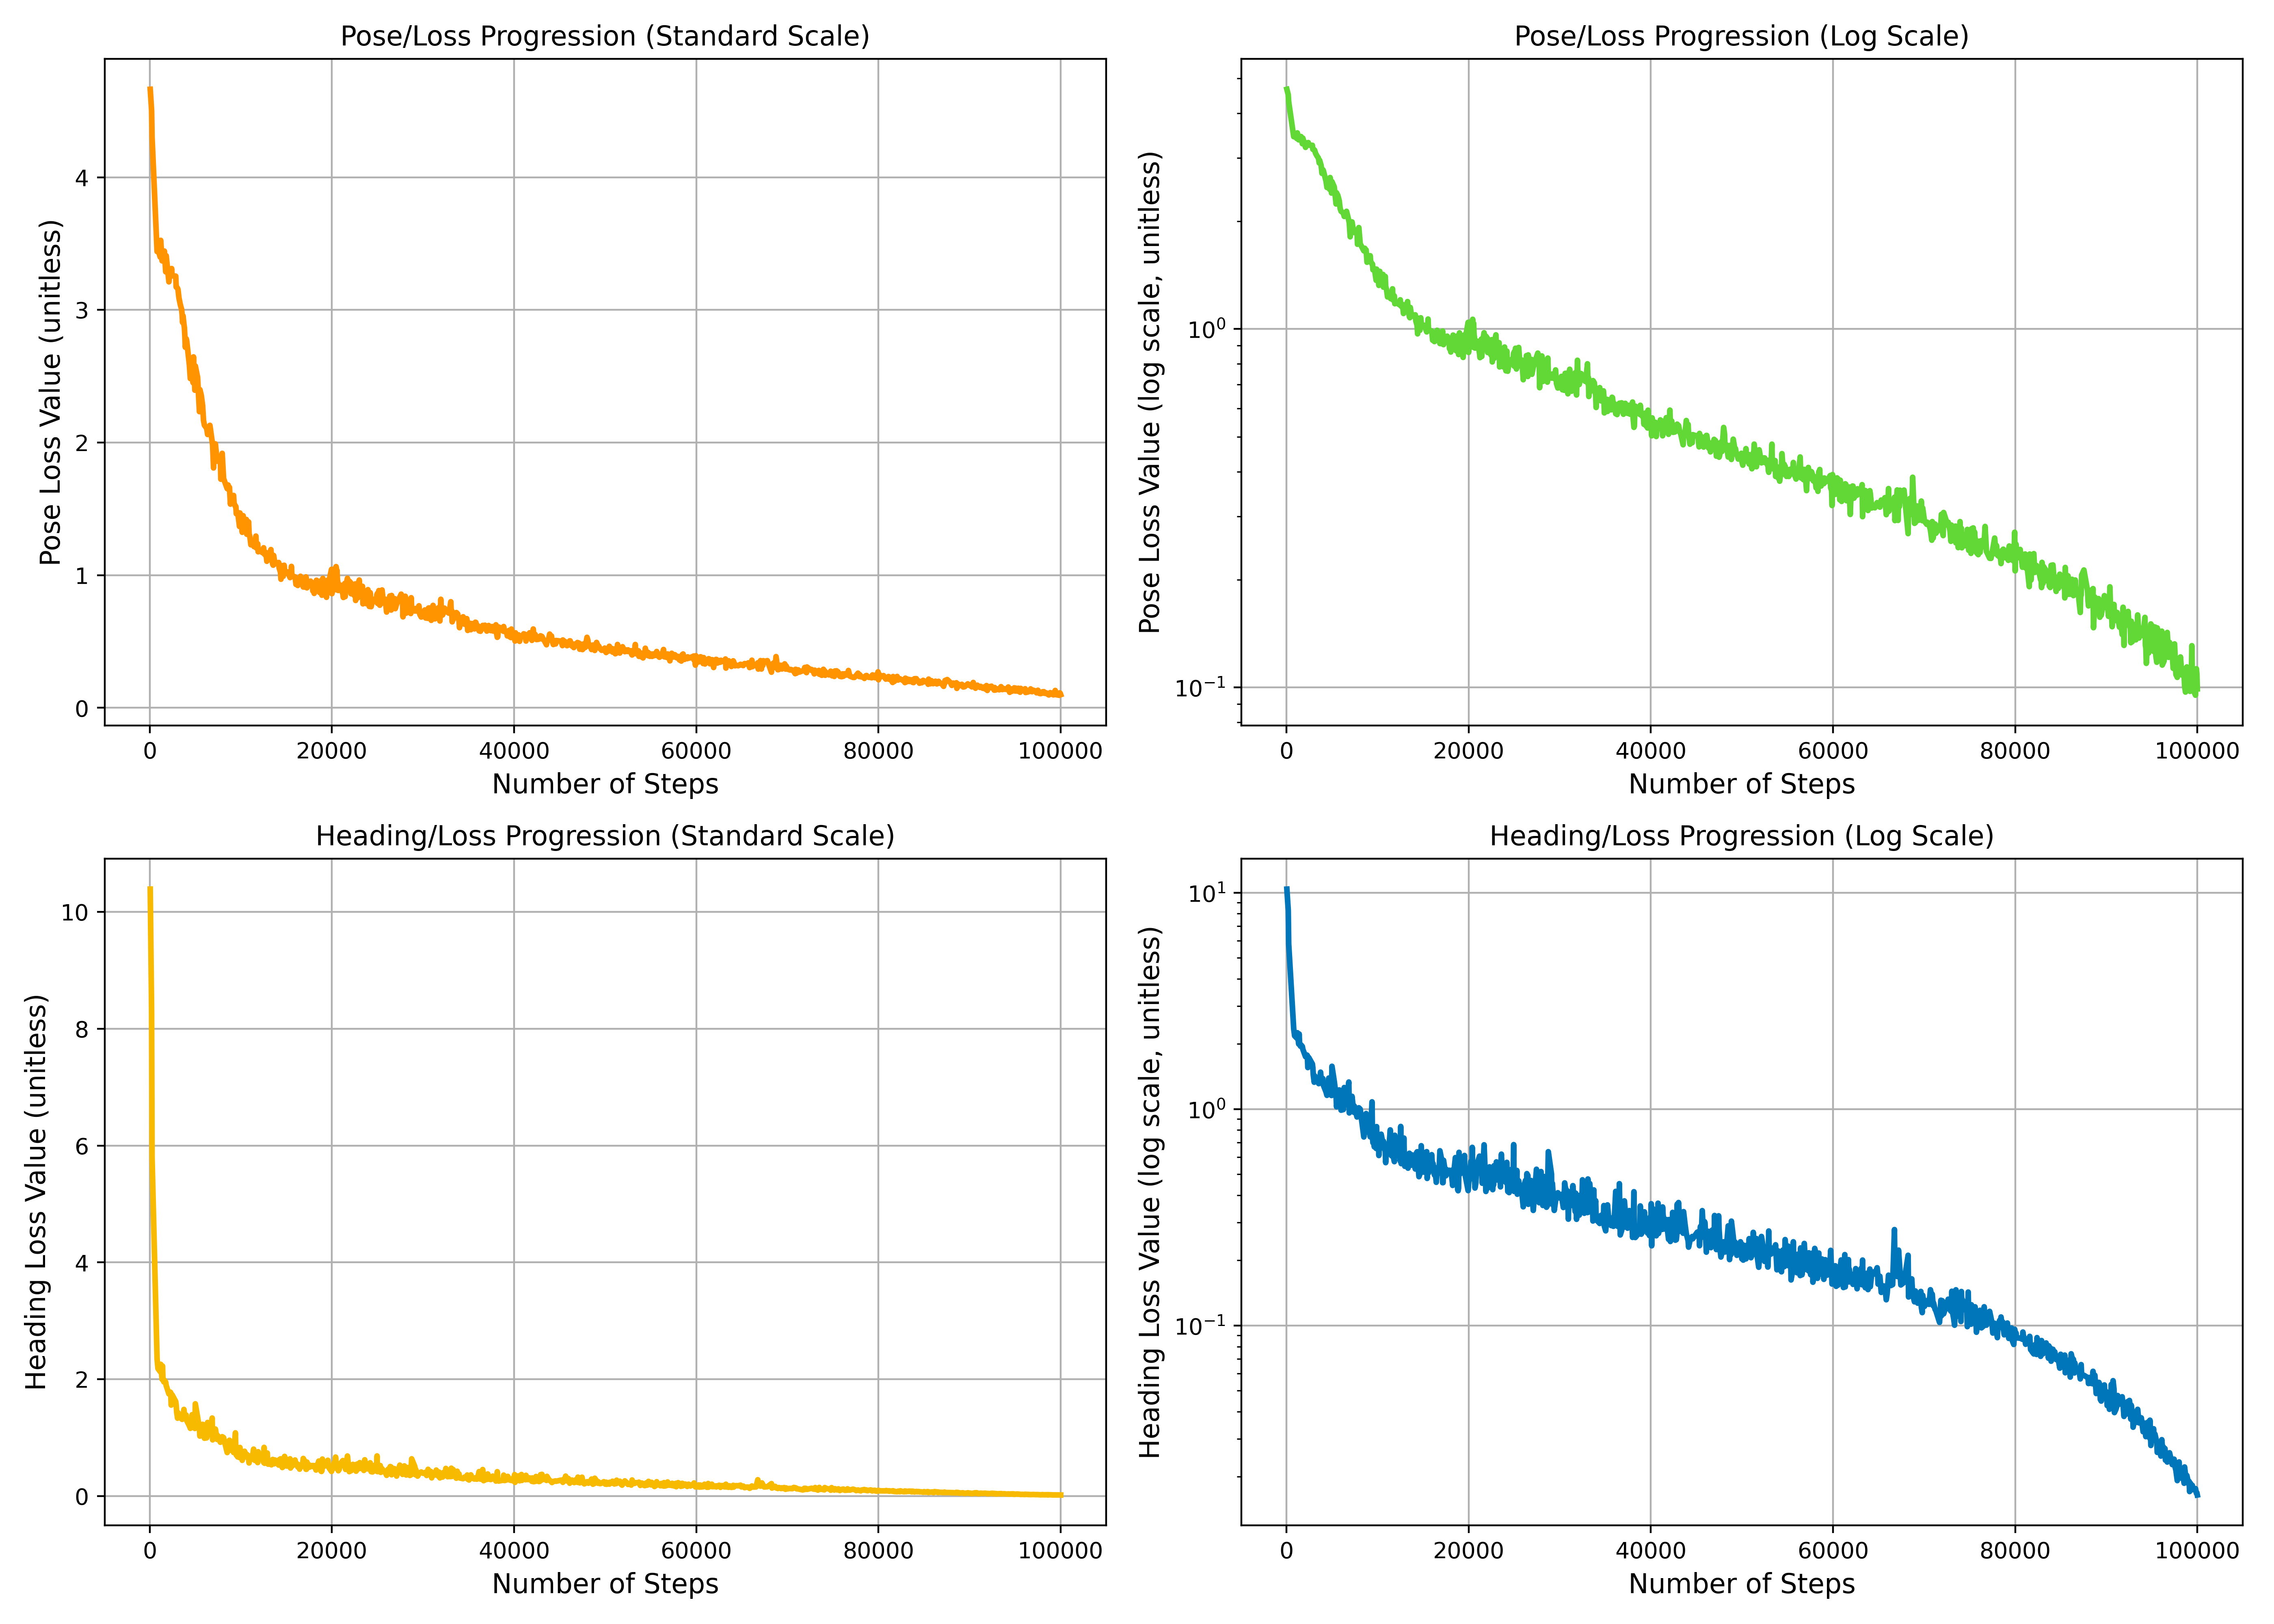
\includegraphics[width=1\linewidth]{LateX//figs/l1s_111_DEG_pose_heading_loss_comparison.png}
    \caption{Comparison of Pose (orange) and Heading (yellow) losses during training. The plot features a standard scale on the left and a logarithmic scale on the right, highlighting a greater contribution of the heading loss.}
    \label{fig:deg-l1s-loss-comparison}
\end{figure}

Converting the heading angle to degrees, as expected, led to improved results by reducing errors and aligning predicted values more closely with the desired targets. Once again, the Smooth L1 loss demonstrated superior generalization performance.

\subsection*{Full Dataset Split with Heading Angle in Degrees}
As mentioned at the beginning of this section, the previous attempts were conducted without utilizing the entire available dataset. Based on the results from the preliminary experiments, the full dataset was later employed by merging all sequences from the three streets. To ensure the most effective evaluation, only the best-performing model, from the initial analysis, which was trained with the Smooth L1 loss function, was selected for testing. 

Figure~\ref{fig:total-loss-progression} illustrates the improvements in angle prediction, which are attributed to the increased dataset size, the application of Smooth L1 loss, and the conversion of angles to degrees. Despite these advancements, significant challenges persist in addressing translation errors. While the current approach shows promise and demonstrates improvements, achieving precise HD map alignment will likely require further model refinement or still using the implementation of optimization techniques. This model version has the potential to assist in complex scenarios, but it does not fully resolve the offline localization process.
\begin{figure}[H]
    \centering
    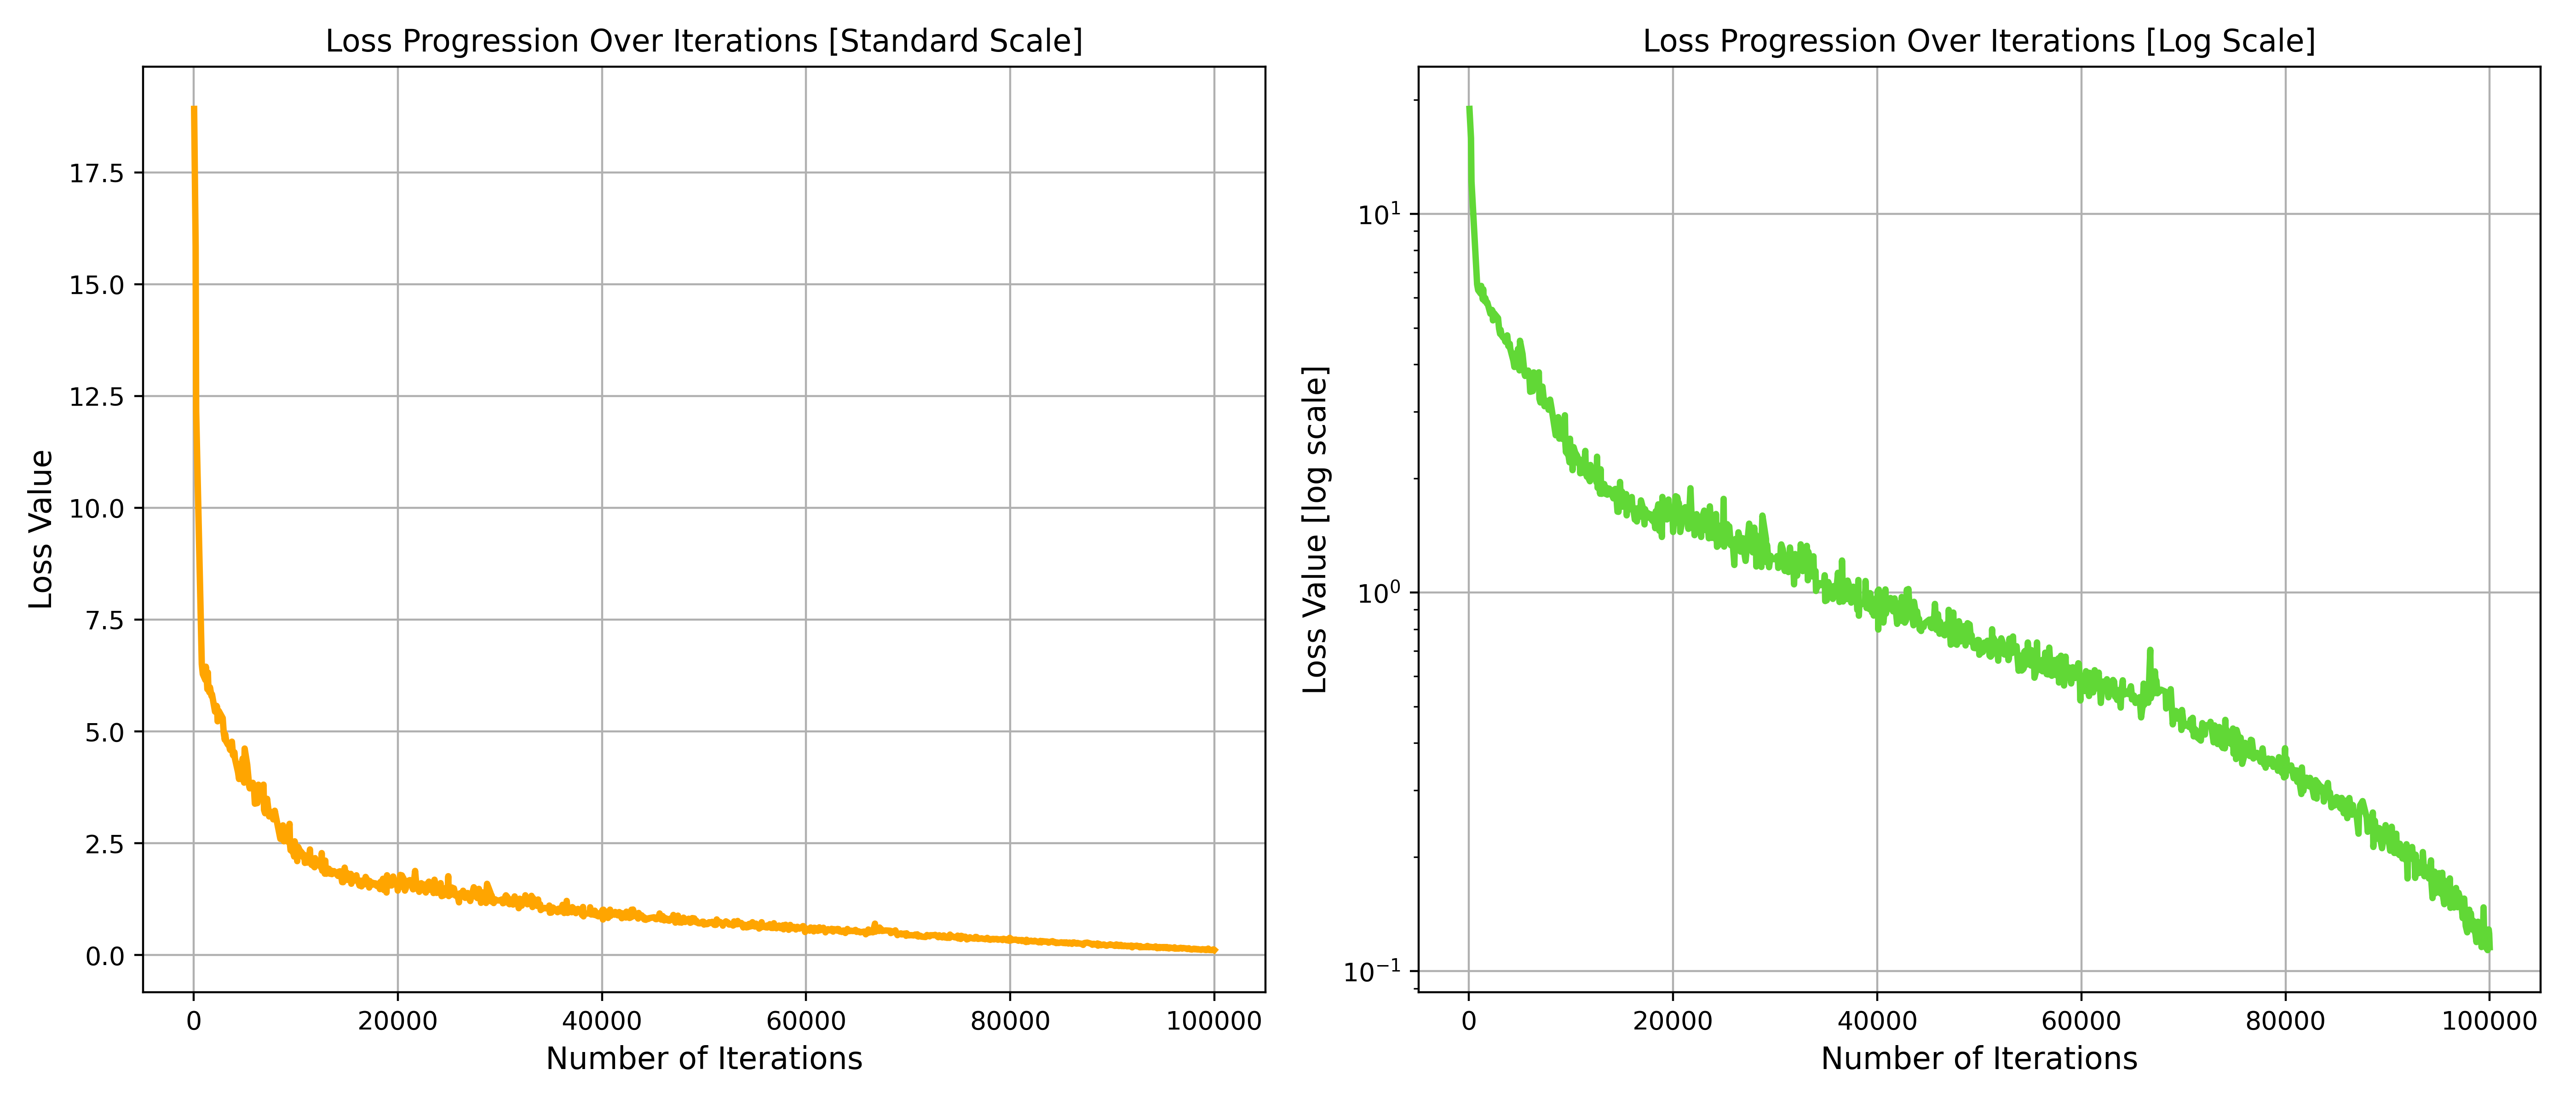
\includegraphics[width=1\linewidth]{loss_total_l1sDEG_progression_comparison.png}
    \caption{Progression of total loss with Smooth L1 Loss (Heading in degrees).}
    \label{fig:total-loss-progression}
\end{figure}

The results indicate that the contributions of heading and translation errors are approximately balanced in this case, which may explain the observed improvements in heading accuracy.
\begin{figure}[H]
    \centering
    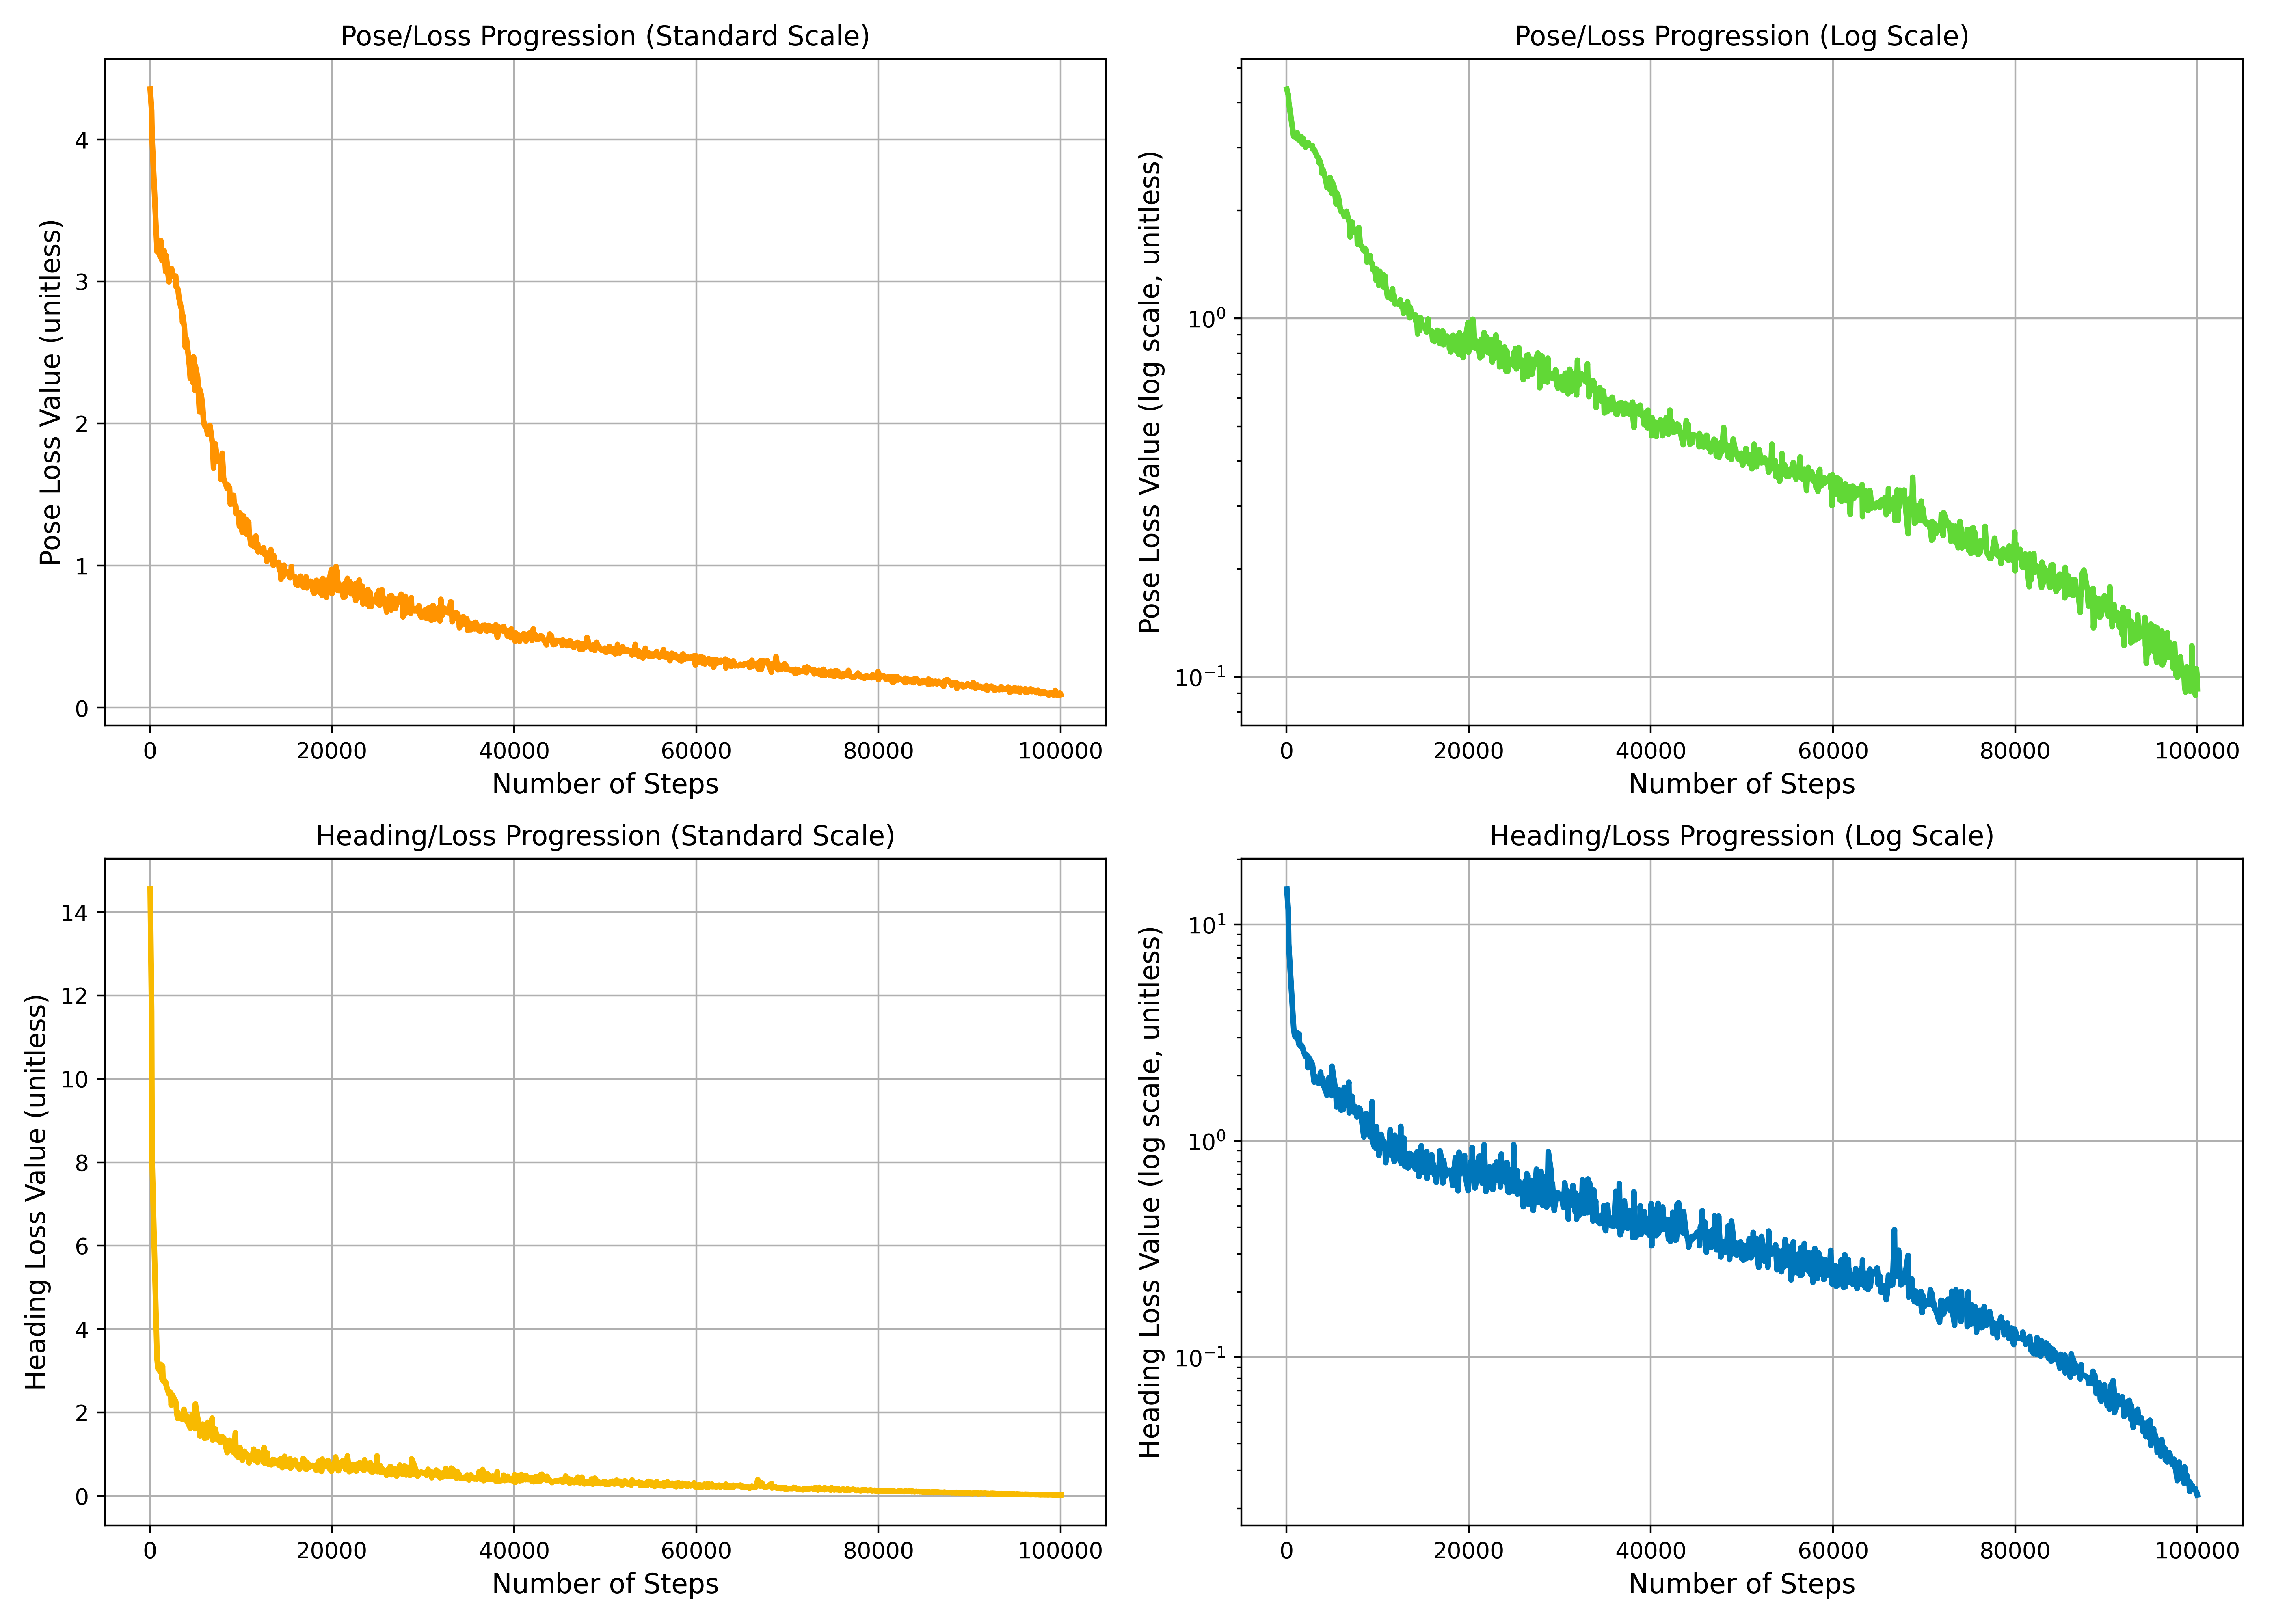
\includegraphics[width=1\linewidth]{LateX//figs/l1sDEG_pose_heading_loss_comparison.png}
    \caption{Comparison of pose heading loss across different iterations.}
    \label{fig:pose-heading-loss-2}
\end{figure}

A summary of the results obtained during different evaluation stages, as iterations progress, is provided in Table~\ref{tab:pose_variations_final_sumup}.

\begin{table}[H]
    \centering
    \scriptsize
    \renewcommand{\arraystretch}{1.2}
    \setlength{\tabcolsep}{10pt} 
    \begin{tabular}{c c c c c}
        \toprule
        \textbf{Iteration} & \textbf{$\Delta$ Pose [m]} & \textbf{$\Delta \theta$ [deg]} & \textbf{$\Delta x + \Delta y$ [m]} & \textbf{$\Delta h$ [m]} \\
        \midrule
        \num{10000}   & 2.35 & 1.70  & 2.21 & 0.14 \\
        \num{20000}   & 2.16 & 1.04  & 1.88 & 0.28 \\
        \num{30000}   & 2.09 & 1.02  & 2.02 & 0.06 \\
        \num{40000}   & 1.90 & 0.85  & 1.89 & 0.016 \\
        \num{60000}   & 1.75 & 0.85  & 1.74 & 0.006 \\
        \num{80000}   & 1.66 & 0.77  & 1.66 & 0.00 \\
        \num{100000}  & \textbf{1.61} & \textbf{0.74}  & \textbf{1.61} & \textbf{0.00} \\
        \bottomrule
    \end{tabular}
    \caption{Evaluation (L1) values in pose, angle (in degrees), combined displacement ($\Delta x + \Delta y$), and height across iterations.}
    \label{tab:pose_variations_final_sumup}
\end{table}

\subsection{Inference}
Inference was tested on a new sequence that was not included in the training dataset. This sequence mainly consisted of long, straight roads with few textures or reference points for alignment. The weights used for this test came from the most accurate model analyzed earlier.

During inference, the roto-translation between the map and the car was still applied using data augmentation. This allowed for a visual comparison between the expected target and the predicted results.

The results showed that the network tried to reduce the distance but started from the wrong boundary. This led to a good alignment of the angle but caused the translation to be misaligned by the width of an entire lane. This issue is similar to what can occur with classical optimization methods and represents a scenario that should be avoided. The misalignment is consistent with the evaluation results observed during different stages of training.

The figure below follows the same layout as before, showing the input, the target, and the final prediction in three vertical panels. In this case, the values were not post-processed, so the roto-translation was applied directly to the map instead of the car.
\begin{figure}[H]
    \centering
    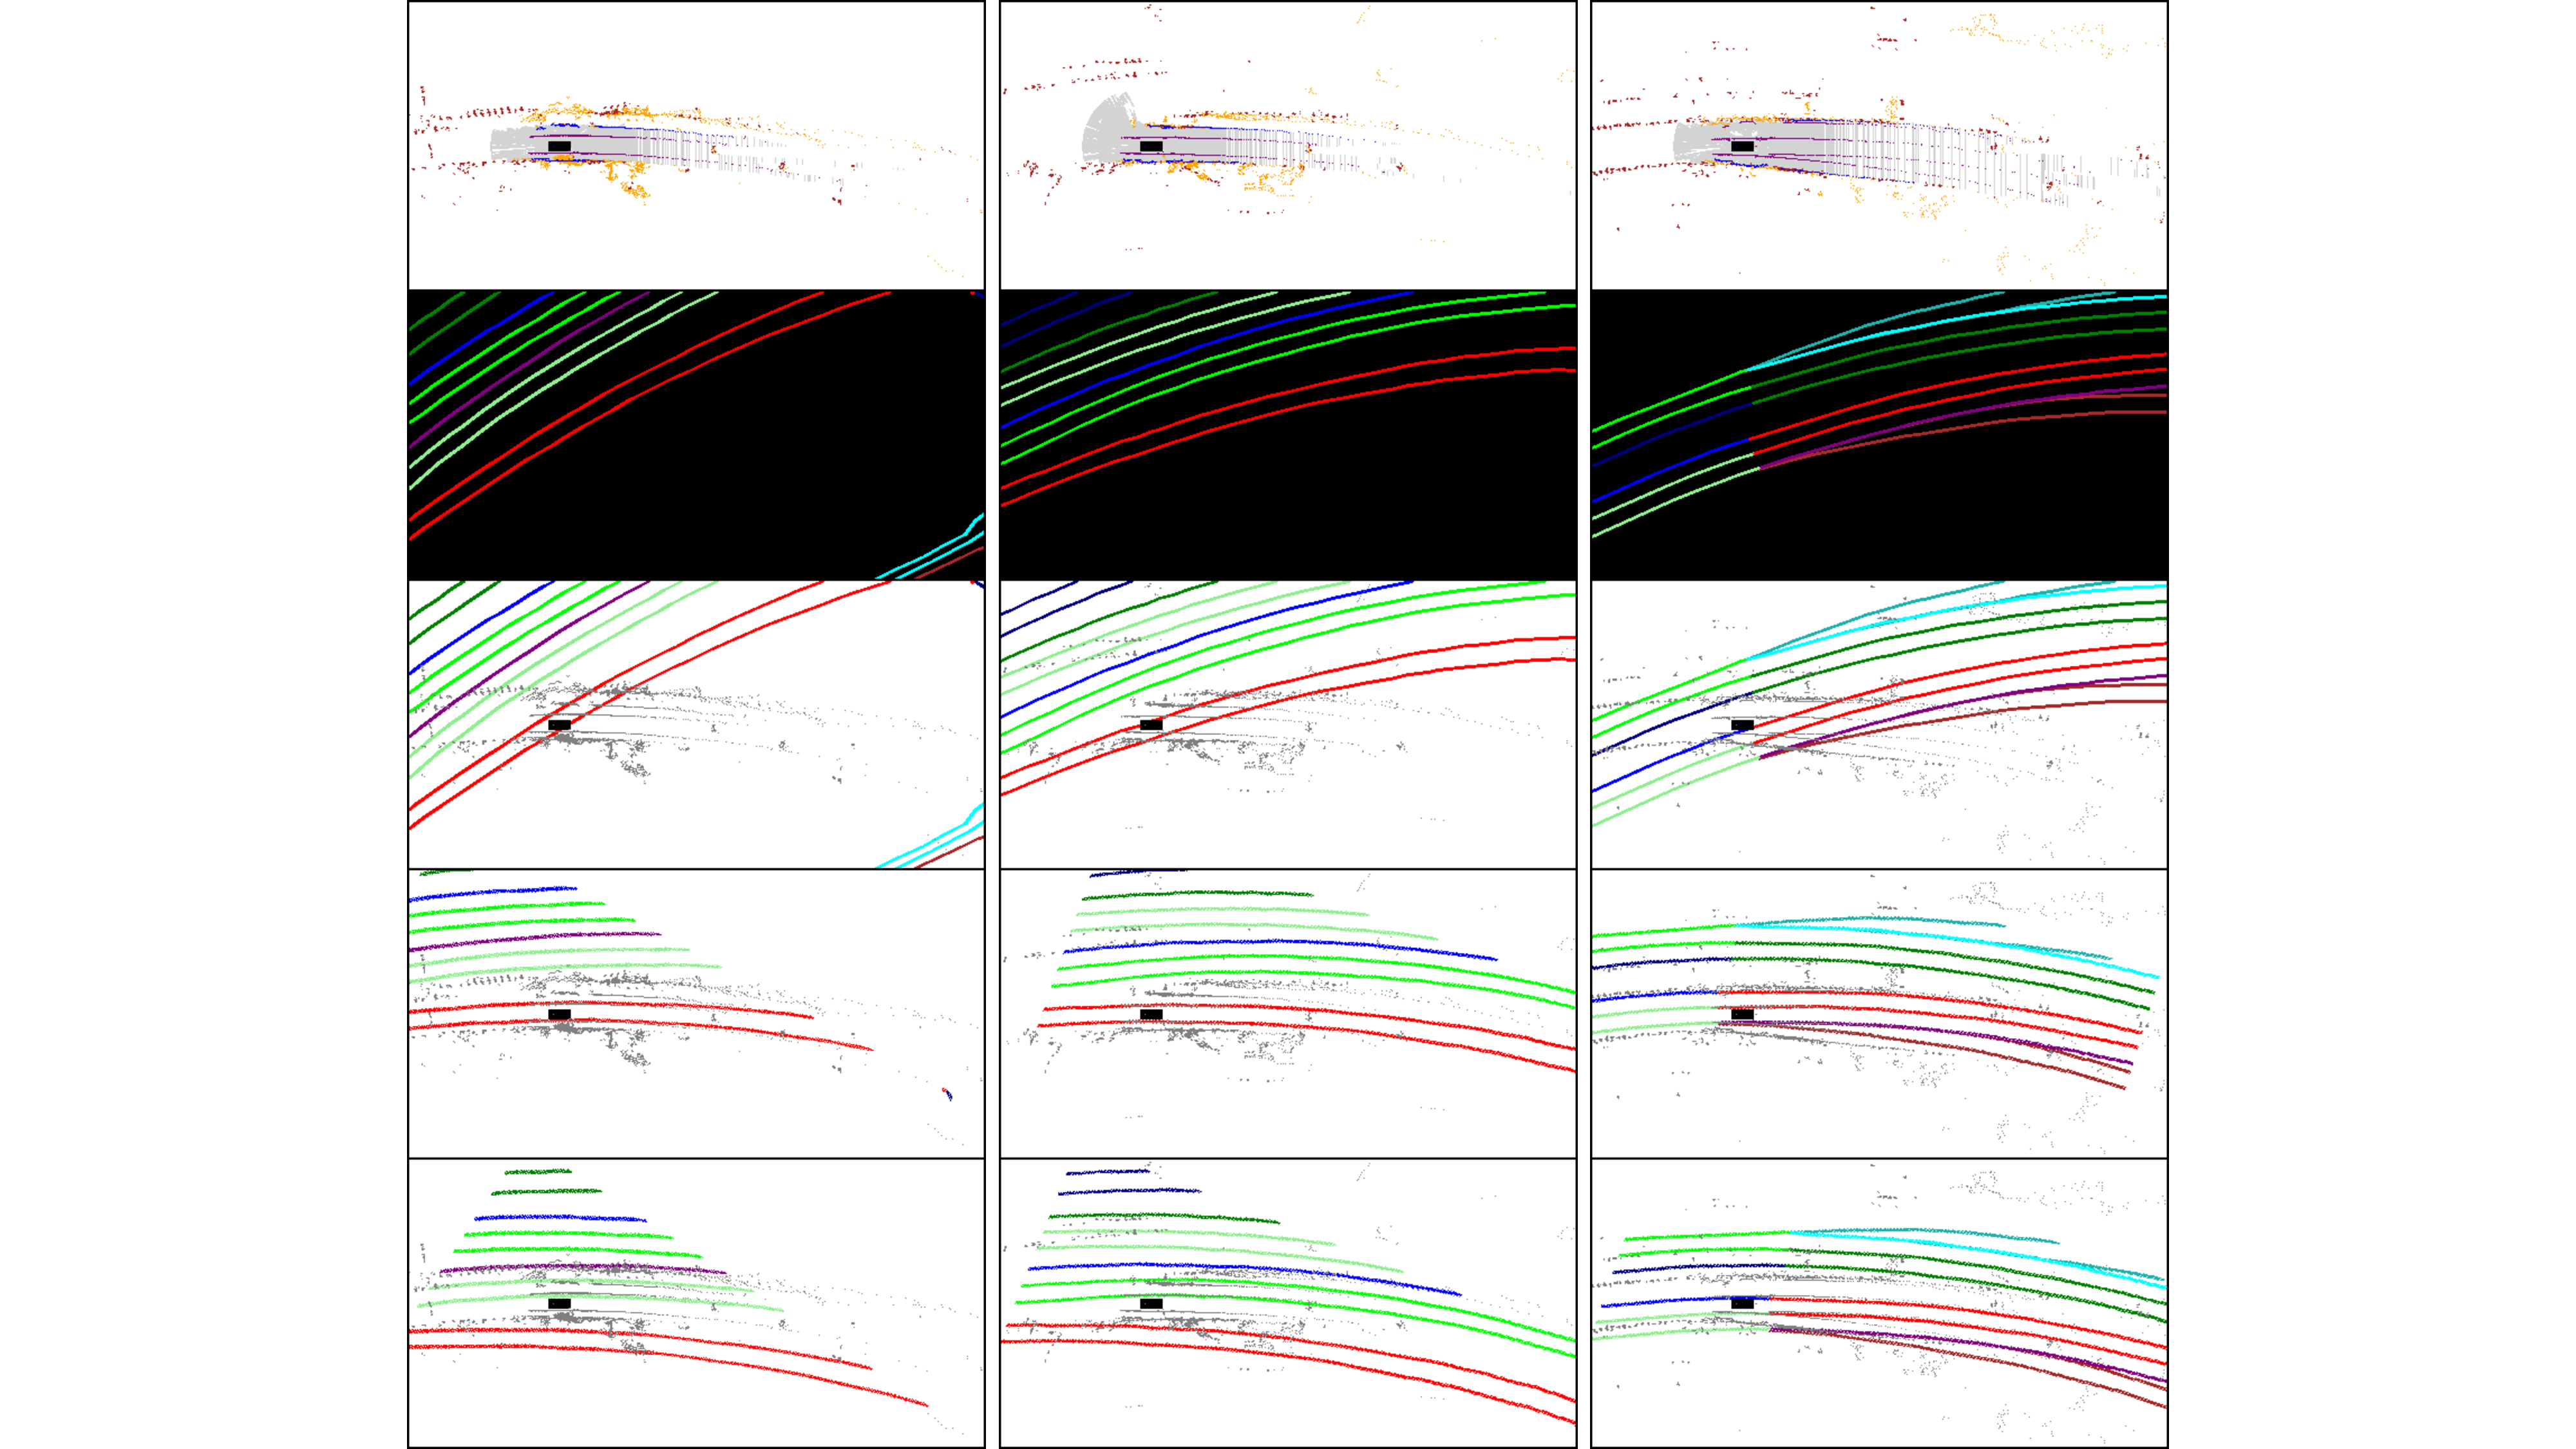
\includegraphics[width=1\linewidth]{Untitled 2.pdf}
    \caption{Example of inference results showing angle alignment but translation error.}
    \label{fig:inference-results}
\end{figure}

\section{Image-Based Localization: BEV Reconstruction}

Based on the results discussed, it became essential to develop an alternative approach to overcome the limitations identified in the initial method. To summarize, the primary issue was the lack of precision in cases where the detectors could not identify sufficient key points, such as on straight roads with minimal texture. This limitation often resulted in unsuccessful alignment. 
Therefore, a new architecture was designed, starting with the reconstruction of a bird’s-eye view (BEV) from the images captured by the vehicle as a preliminary phase. This step is carried out before going on with the previous approach, where the network must align the inputs and outputs the rotation-translation matrix.

As outlined in Subsection (2.2), the inputs to the network now have also ten images: six from long-range stereo cameras and four from short-range stereo cameras. During the BEV reconstruction process, these images are categorized into two groups, creating two different tensors: short-range and long-range.
\begin{figure}[H]
    \centering
    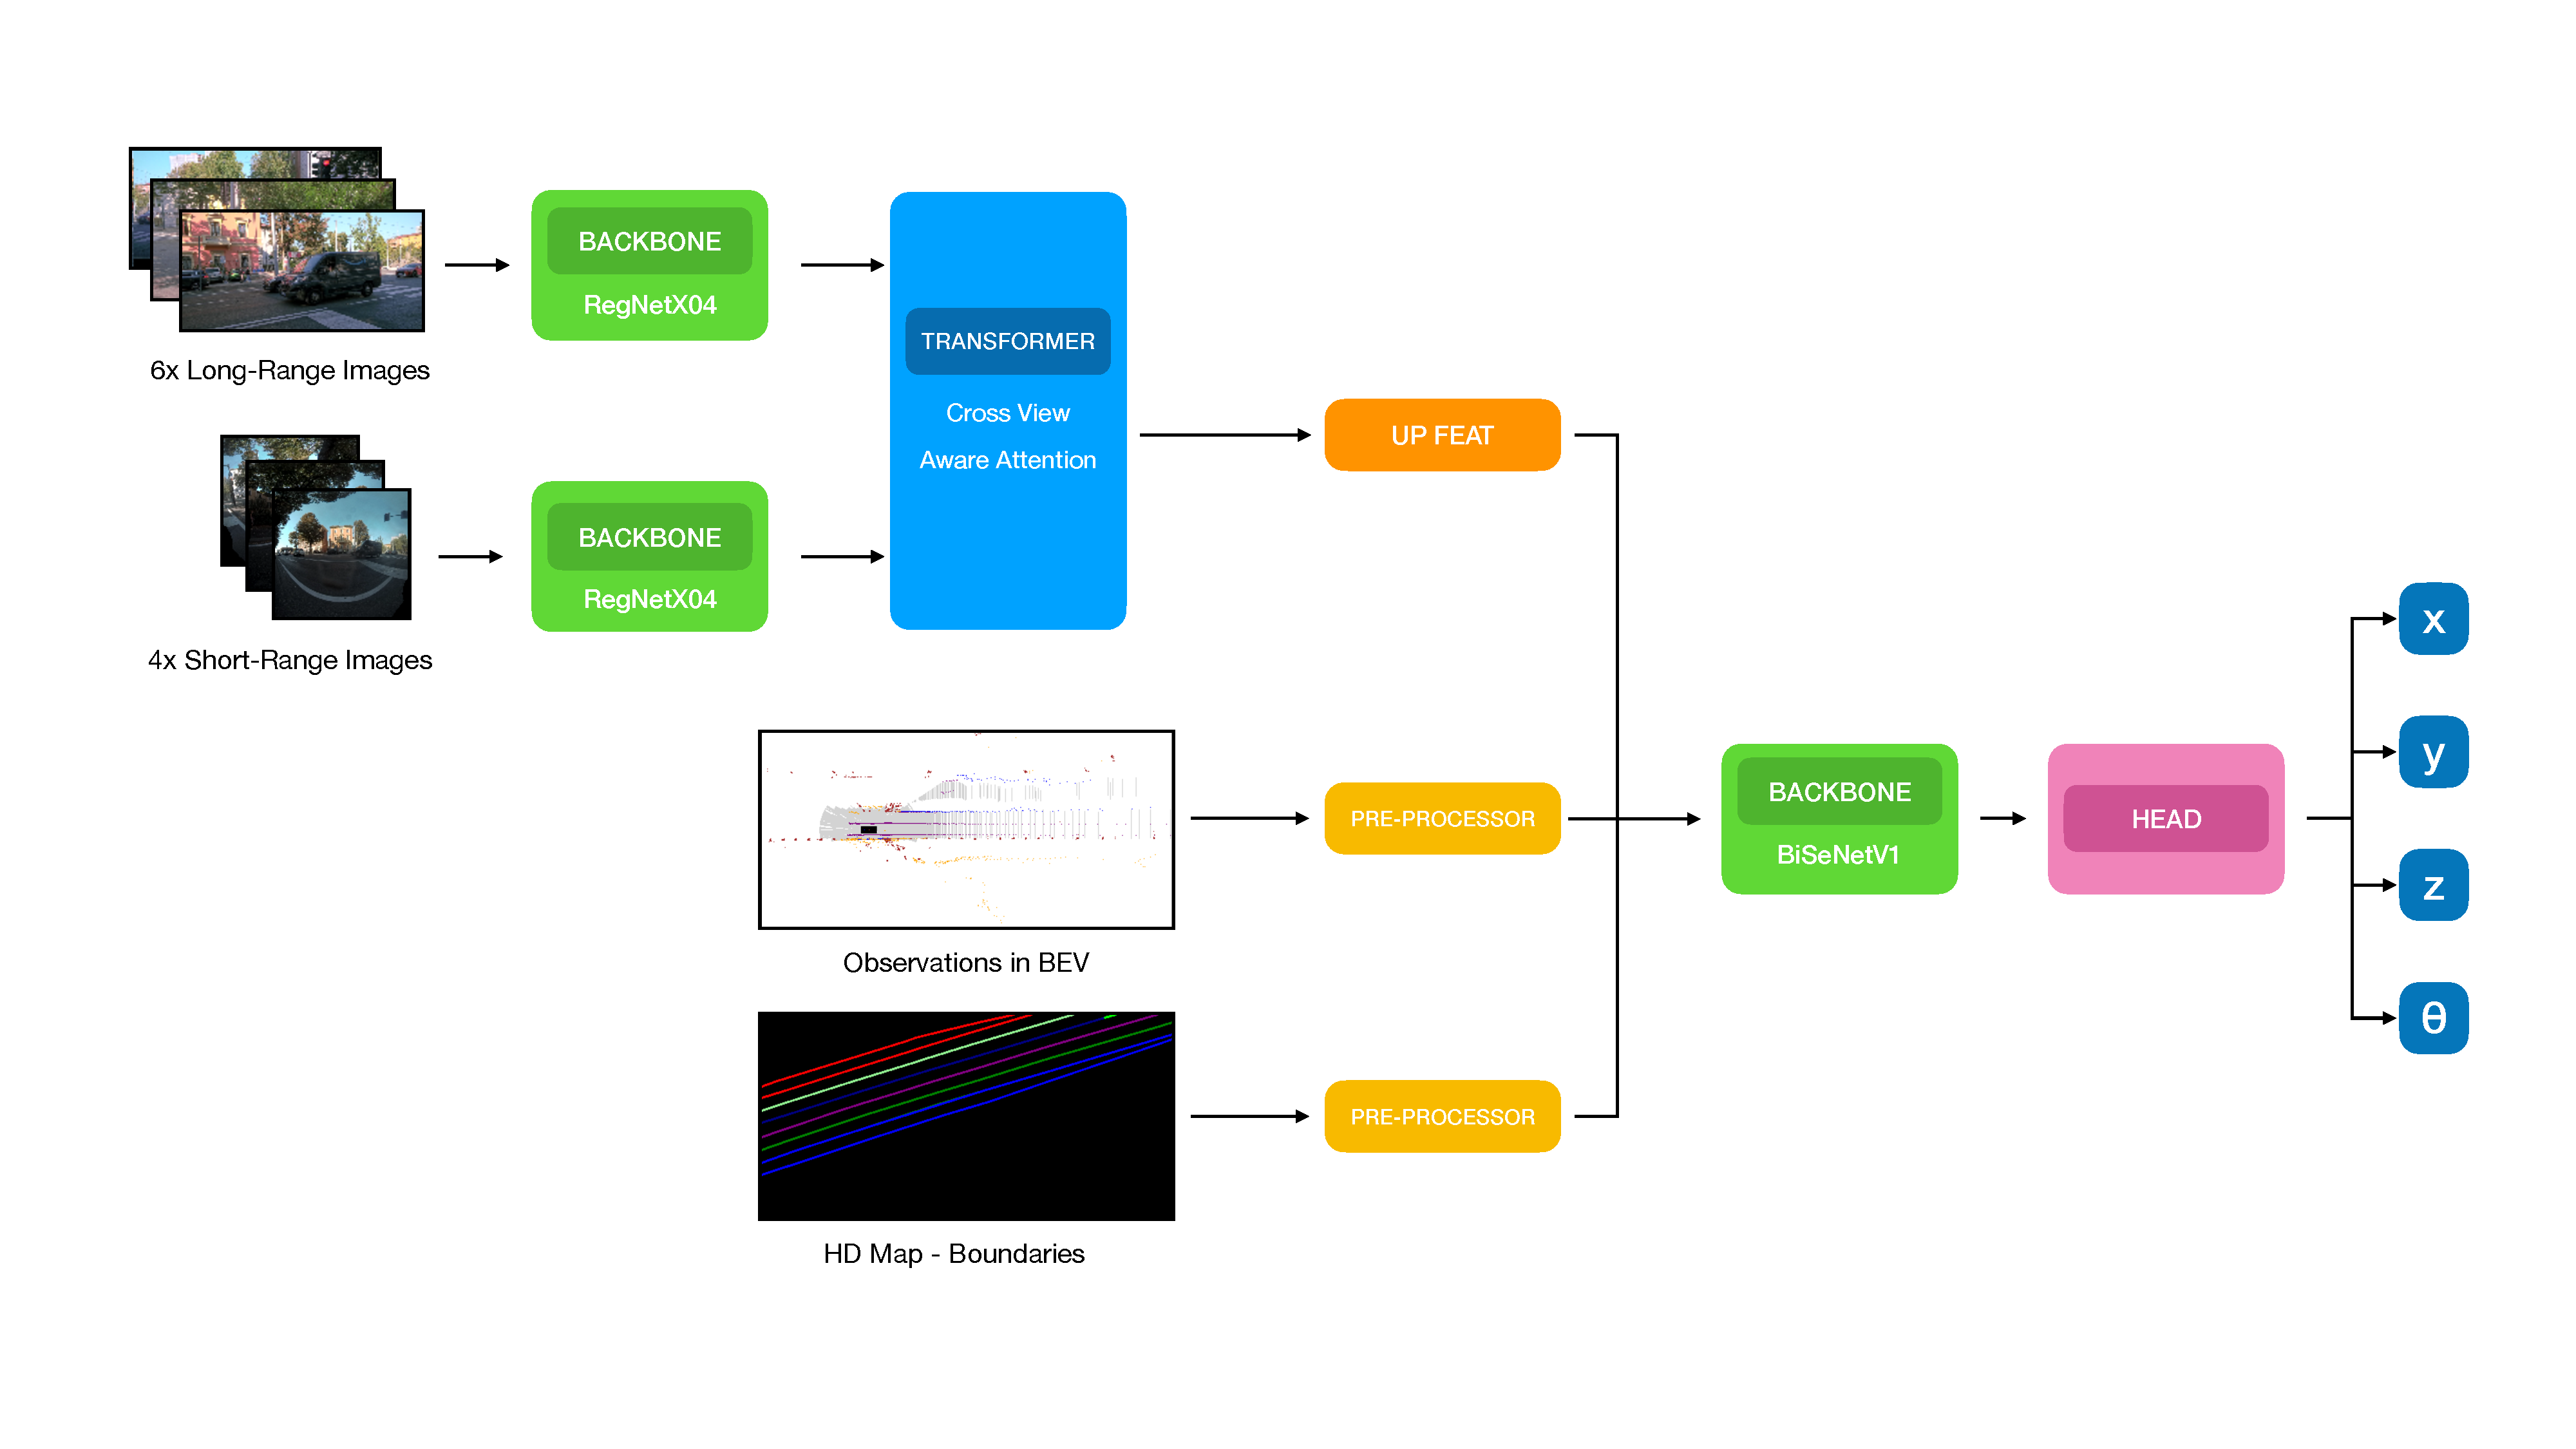
\includegraphics[width=1\linewidth]{LateX//figs/architecture2.pdf}
    \caption{Overview of the complete model architecture, illustrating input processing, BEV reconstruction, feature extraction, and output generation.}
    \label{fig:bev-architecture}
\end{figure}

\subsection*{Bird’s-Eye View Reconstruction}
To reconstruct the bird’s-eye view (BEV), the images—grouped into tensors are passed through backbones to extract features. 

The chosen backbone for this task is RegNetX, a model designed to improve ResNet and its variants, widely used in computer vision tasks. While ResNet facilitates efficient gradient flow through shortcut connections, its additive approach limits the exploration of complementary features. RegNetX addresses this by introducing a regulator module that acts as a memory mechanism, enabling the extraction of complementary features and enhancing spatio-temporal feature extraction capabilities.

For this implementation, a specific version of RegNetX was used. This model is designed with a linear parameterization of block widths across the network, ensuring consistency and simplicity. Additional constraints, such as fixed bottleneck ratios, width multipliers, and initial widths, further optimize the model structure. These features enable high performance while minimizing computational requirements, outperforming a classical ResNet approach with fewer parameters and less computational power (see Figure~\ref{fig:regnetvsresnet}) \cite{Radosavovic2020}.

\begin{figure}[H]
    \centering
    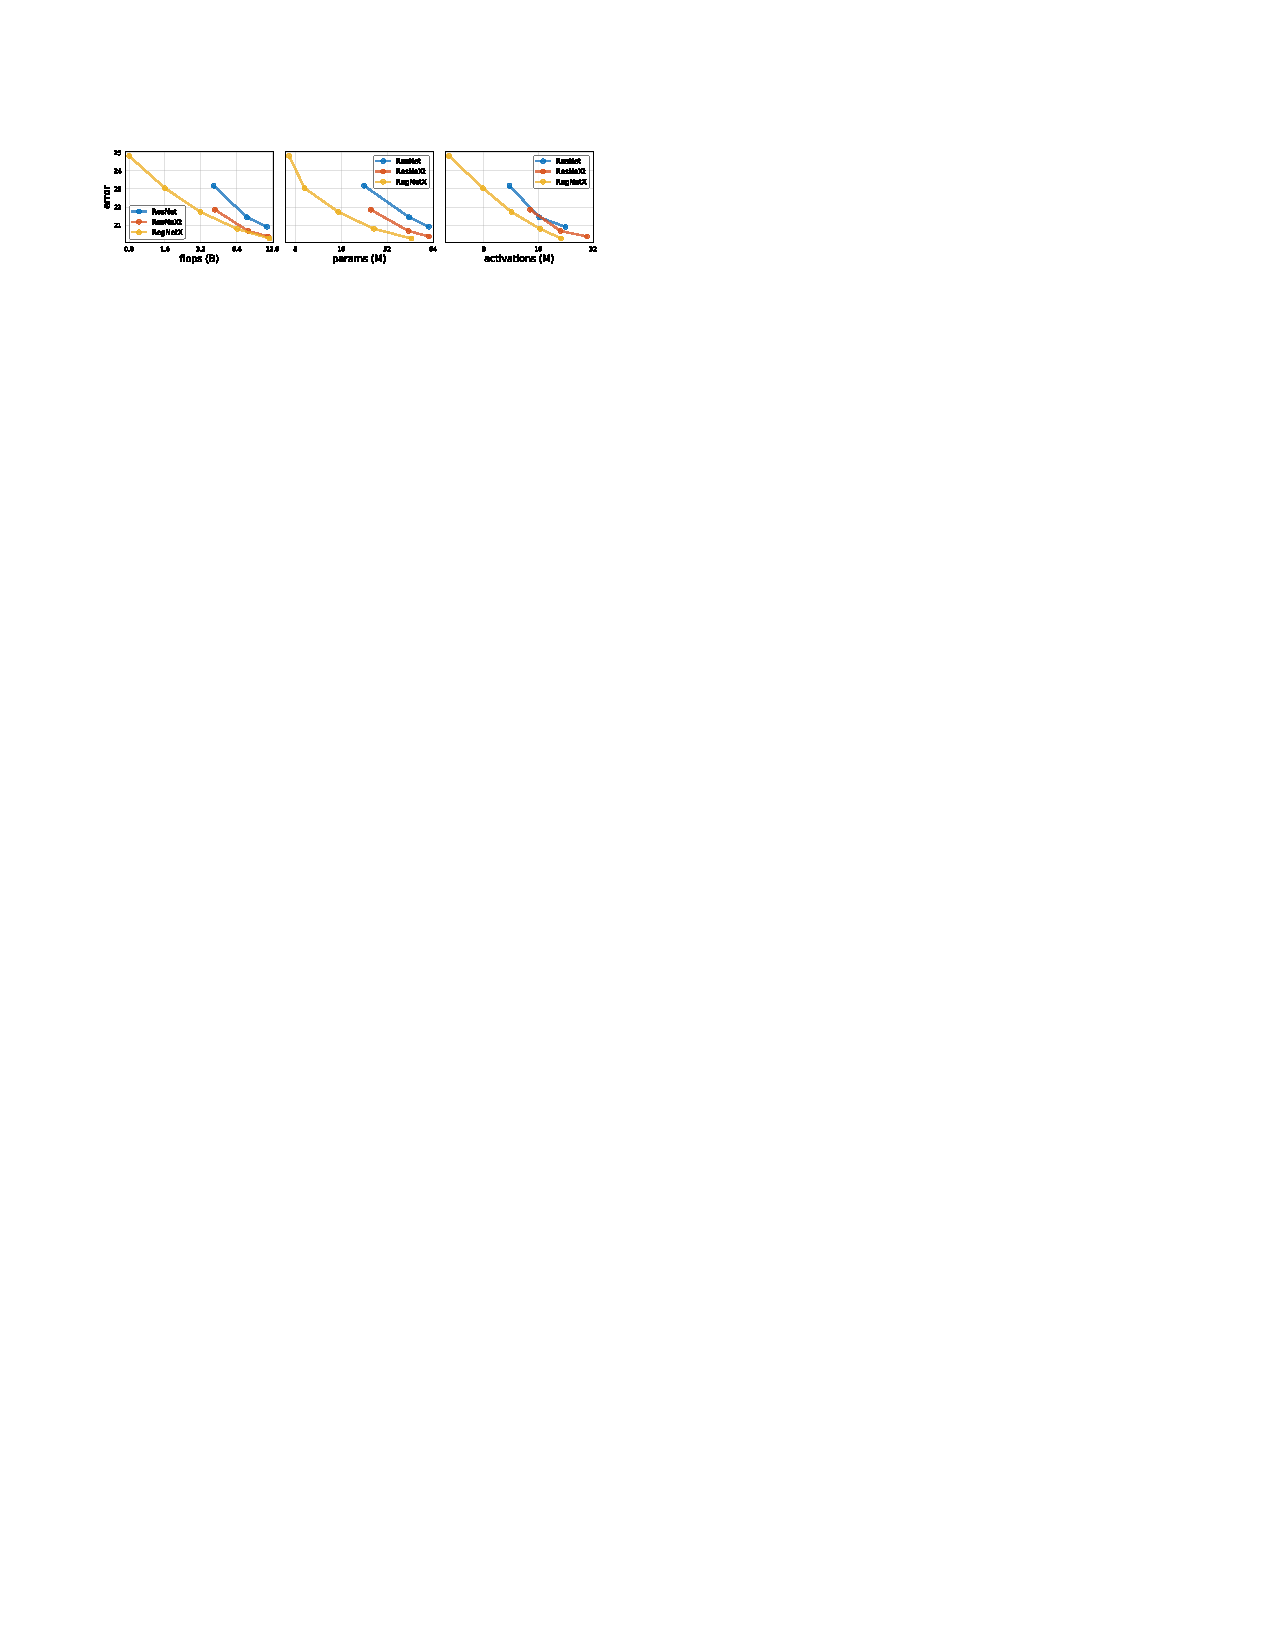
\includegraphics[width=1\linewidth]{Radosavovic_Designing_Network_Design_Spaces_CVPR_2020_paper (2).pdf}
    \caption{Comparison of RegNetX and ResNet in terms of performance and computational efficiency \cite{Radosavovic2020}.}
    \label{fig:regnetvsresnet}
\end{figure}

The BEV (Bird’s Eye View) network uses a transformer module to process both long-range and short-range features, generating a unified BEV representation. As discussed in Section 2, a transformer is particularly effective when fusing data from different modalities, making it well-suited for the BEV representation, where data from $10$ cameras contribute to the same task, considering also that different cameras contribute to the same part of the reconstruction. 
The key components and their roles in this process are:

\begin{itemize}
    \item \textbf{Camera Position Encoder} (\texttt{self.cam\_pos\_encoder}): Encodes the positional information of the cameras, enabling the network to understand spatial relationships between them;
    \item \textbf{Query Encoder} (\texttt{self.query\_encoder}): Generates query embeddings derived from BEV queries.
    \item \textbf{Key Encoders}:
    \begin{itemize}
        \item \textbf{Long-Range Key Encoder} (\texttt{self.key\_encoder}): Encodes key embeddings from long-range camera features.
        \item \textbf{Short-Range Key Encoder} (\texttt{self.key\_encoder}): Reuses the same encoder for short-range camera features.
    \end{itemize}
    \item \textbf{Value Encoders}:
    \begin{itemize}
        \item \textbf{Long-Range Value Encoder} (\texttt{self.value\_encoder\_long}): Converts long-range camera features into value embeddings.
        \item \textbf{Short-Range Value Encoder} (\texttt{self.value\_encoder\_short}): Converts short-range camera features into value embeddings.
    \end{itemize}
    \item \textbf{Cross-Attention Module} (\texttt{self.cross\_att}): Conducts cross-attention between the query embeddings and the key-value pairs from both long-range and short-range features, enabling feature fusion.
\end{itemize}

\begin{figure}[H]
    \centering
    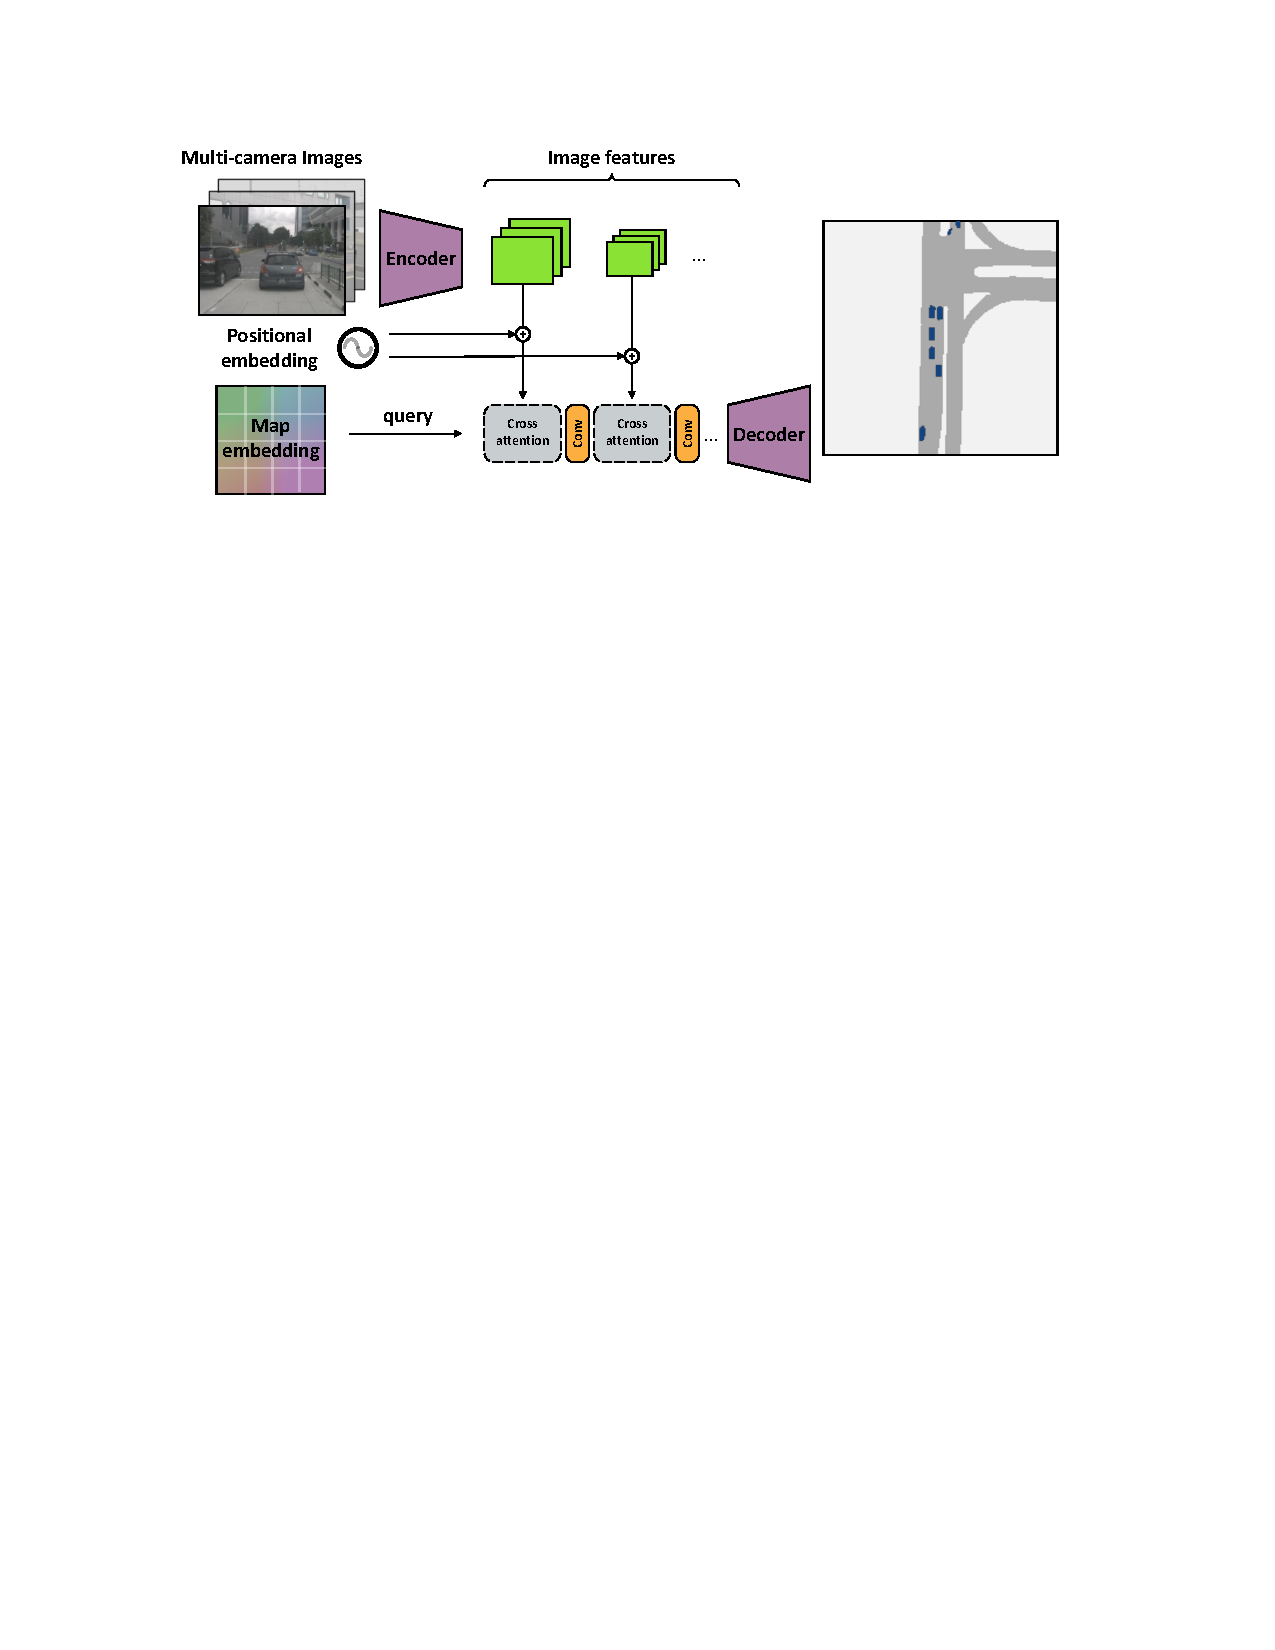
\includegraphics[width=1\linewidth]{LateX//figs/2205.02833v1.pdf}
    \caption{Architecture of the cross-view attention mechanism used in the transformer \cite{zhou2022crossviewtransformersrealtimemapview}.}
    \label{fig:bev-transformer}
\end{figure}

In conclusion, the integration of advanced techniques such as cross-attention, positional encoding, and attention masks significantly enhances the model's performance. Cross-attention enables the model to focus on the most relevant parts of the input features by computing attention weights between queries and keys, ensuring efficient feature utilization. Positional encoding introduces spatial information into the embeddings, which is critical for tasks involving spatial reasoning, such as bird’s-eye view transformations. Additionally, attention masks restrict the model's focus to specific regions, further improving its ability to concentrate on pertinent areas.

At this stage, the bird’s-eye view (BEV) reconstruction now becomes part of the inputs that the previous model received. After a series of convolutions to adjust the number of channels and ensure uniformity, the rest of the model architecture remains unchanged. 

Given the performance of earlier models as a reference, the entire available dataset was used, and the same data augmentation techniques were applied. The unique loss function employed was Smooth L1, as it had demonstrated the best performance in previous experiments.

The initial training iterations were configured with the following high-level parameters: data augmentation included body rotations between $-30^\circ$ and $30^\circ$, as well as horizontal and vertical shifts up to $10\%$. The SGD optimizer was used with a base learning rate of \textit{0.1} and a batch size of \textit{32}. The learning rate scheduler followed the \textit{WarmupPolyLR} strategy \cite{kalra2024warmuplearningrateunderlying}, with a warm-up phase lasting $5000$ iterations and a maximum of $100000$ iterations. Automatic Mixed Precision (AMP) was also enabled to improve training efficiency and resource usage.

For this training session, the batch size was reduced due to computational limitations. Specifically, two Tesla V1 GPUs with 32GB of memory each were available, which was insufficient to maintain a batch size of 64. Despite this constraint, excellent results were achieved.

\subsection*{Smooth L1 Loss}

As mentioned, all tests for this architecture were conducted using the Smooth L1 loss function, whose characteristics have been detailed in earlier sections. Based on insights from the previous approach, the heading angle is expressed in degrees, ensuring a scale comparable to the positional changes along the axes. This adjustment simplifies optimization by aligning the scale of all components involved in the loss calculation.

The learning rate progression, shown in Figure~\ref{fig:learning_rate_2}, starts from zero with a warm-up phase, followed by a gradual decrease. This scheduling ensures rapid initial learning while avoiding overshooting and converging smoothly to a local minimum. This controlled progression reflects best practices in deep learning optimization.
\begin{figure}[H]
    \centering
    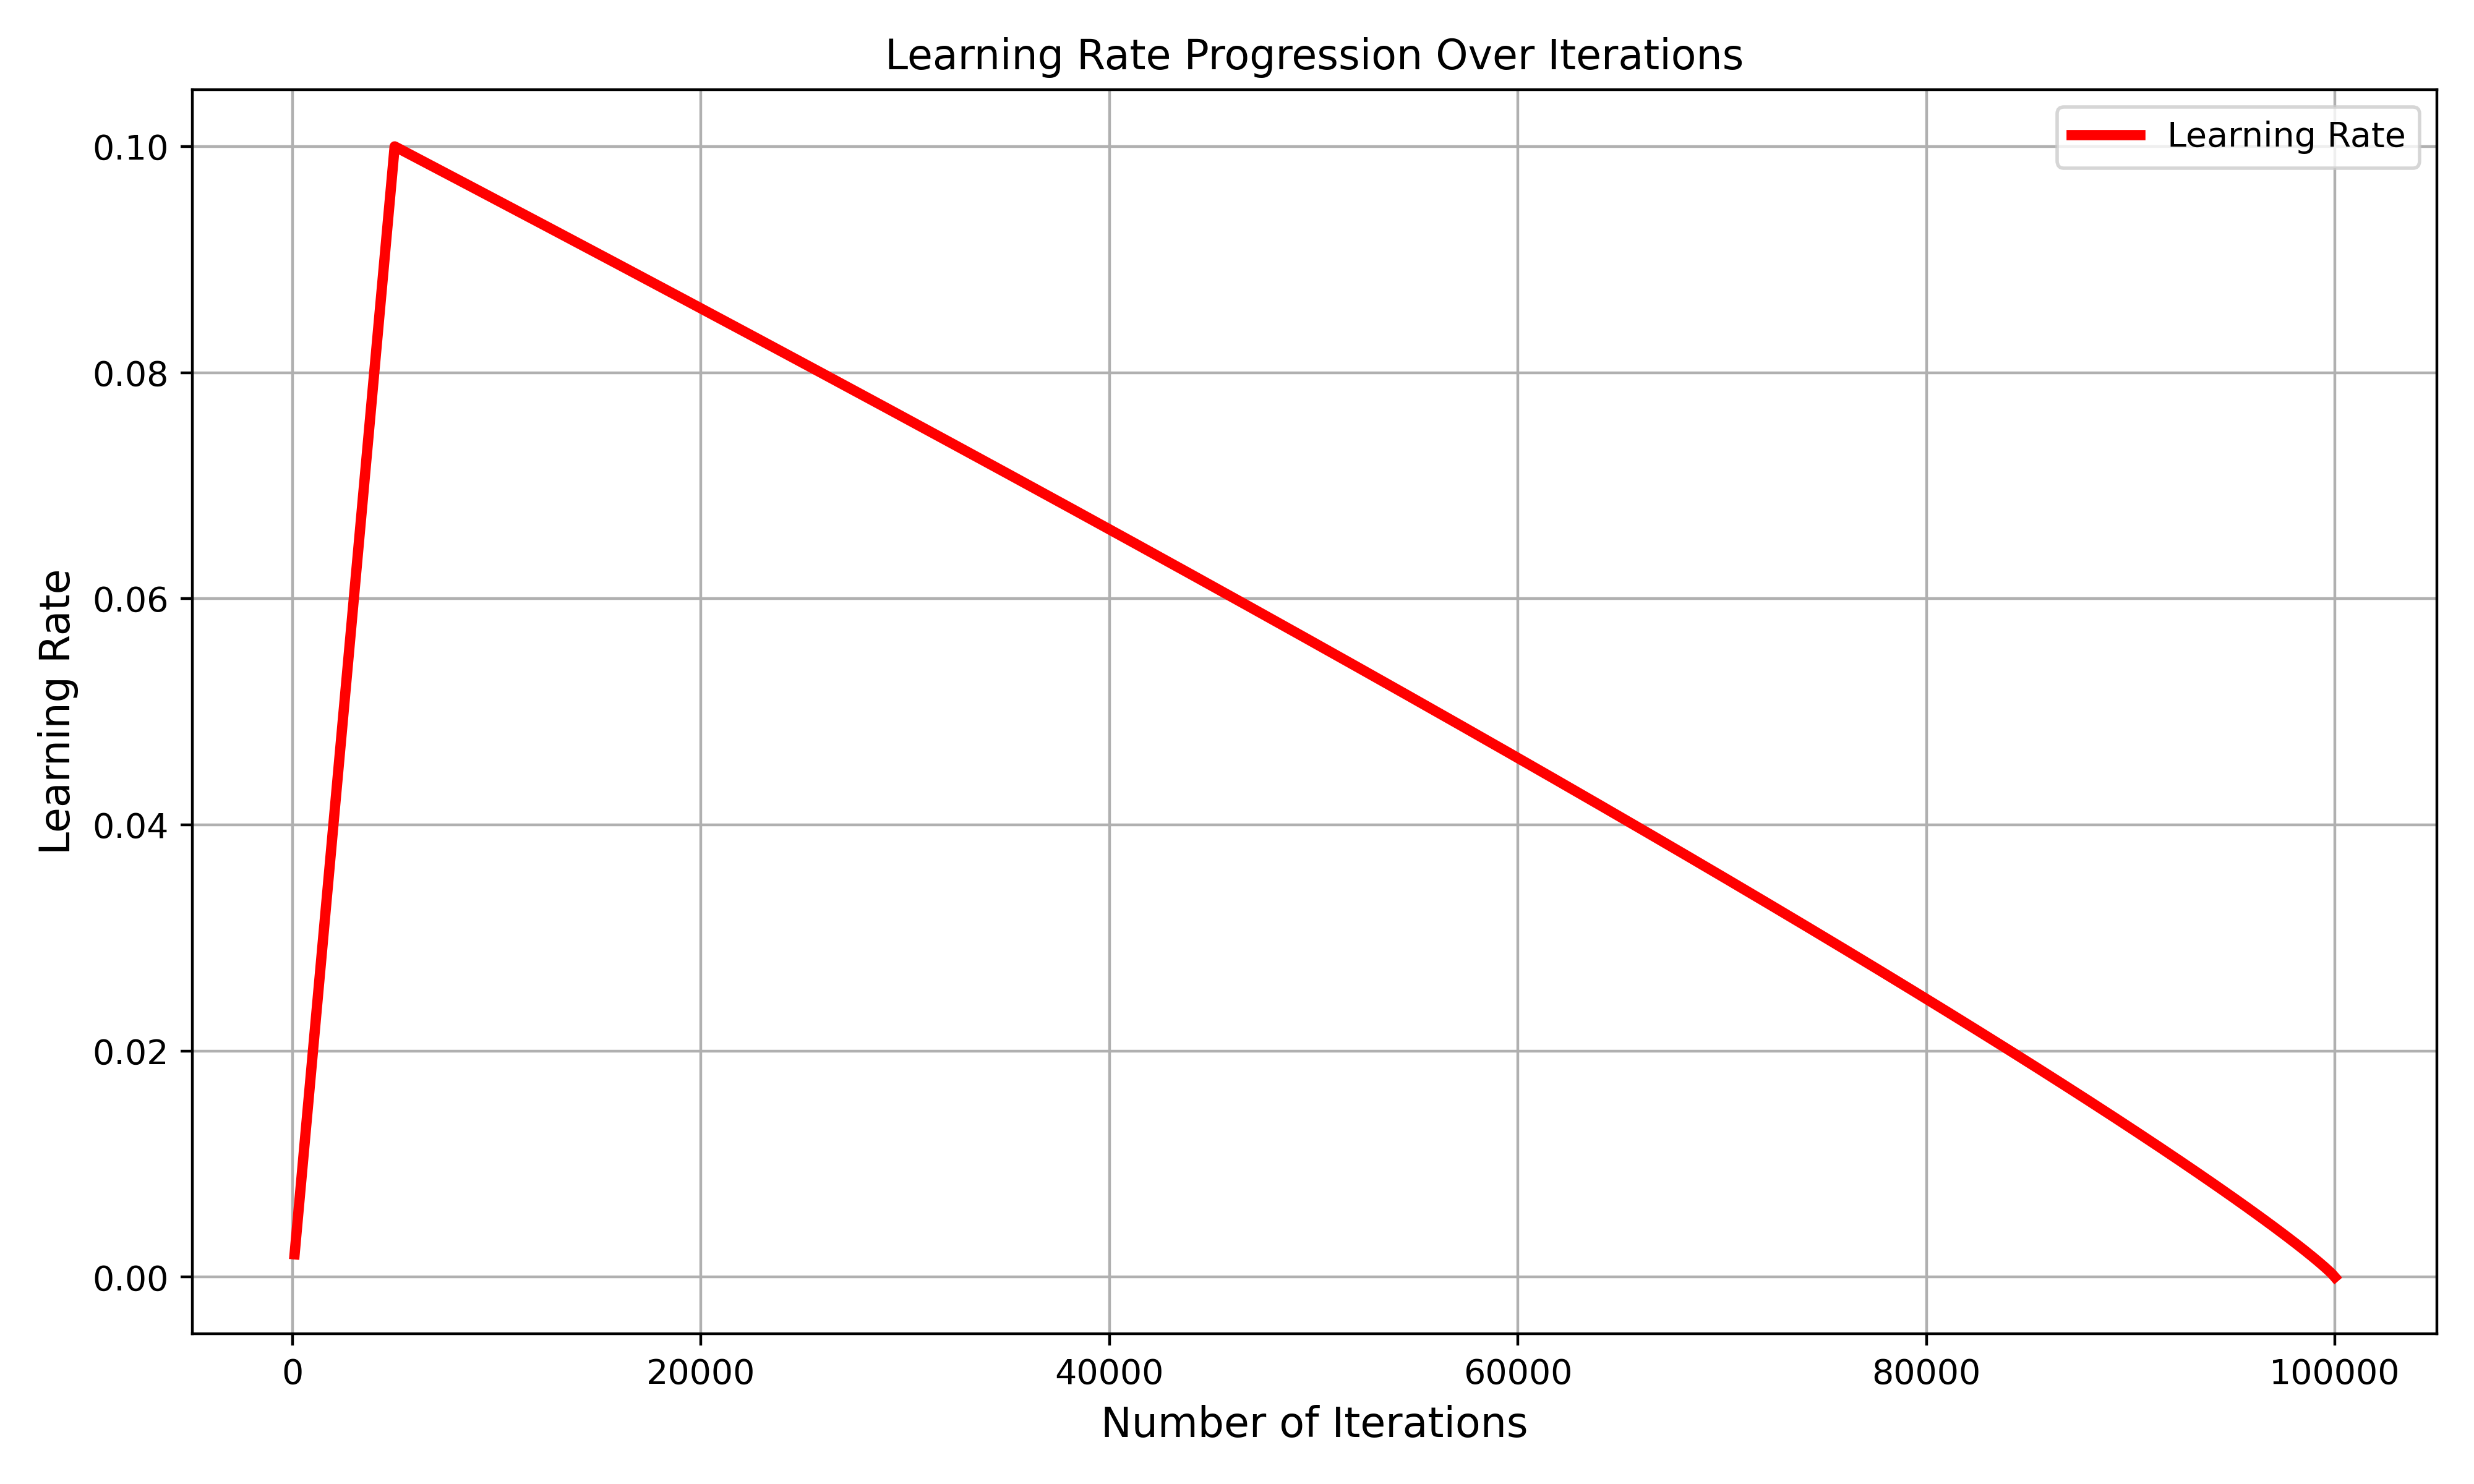
\includegraphics[width=0.75\linewidth]{LateX//figs/BEVlearning_rate_progression.png}
    \caption{Learning rate progression during training, showcasing an initial warm-up phase followed by a gradual decrease. The learning rate peaks at a maximum value of $0.1$ at $5000$ iterations.}
    \label{fig:learning_rate_2}
\end{figure}

The following figure illustrates the training status across two distinct phases: an early stage, where the network was still learning, and a later stage, where the network demonstrates effective learning. In the input section of the figure, the images captured by the car are visible, showcasing both long-range and short-range views. These images highlight the integration of diverse perspectives, crucial for enhancing the alignment process.
\begin{figure}[H]
    \centering
    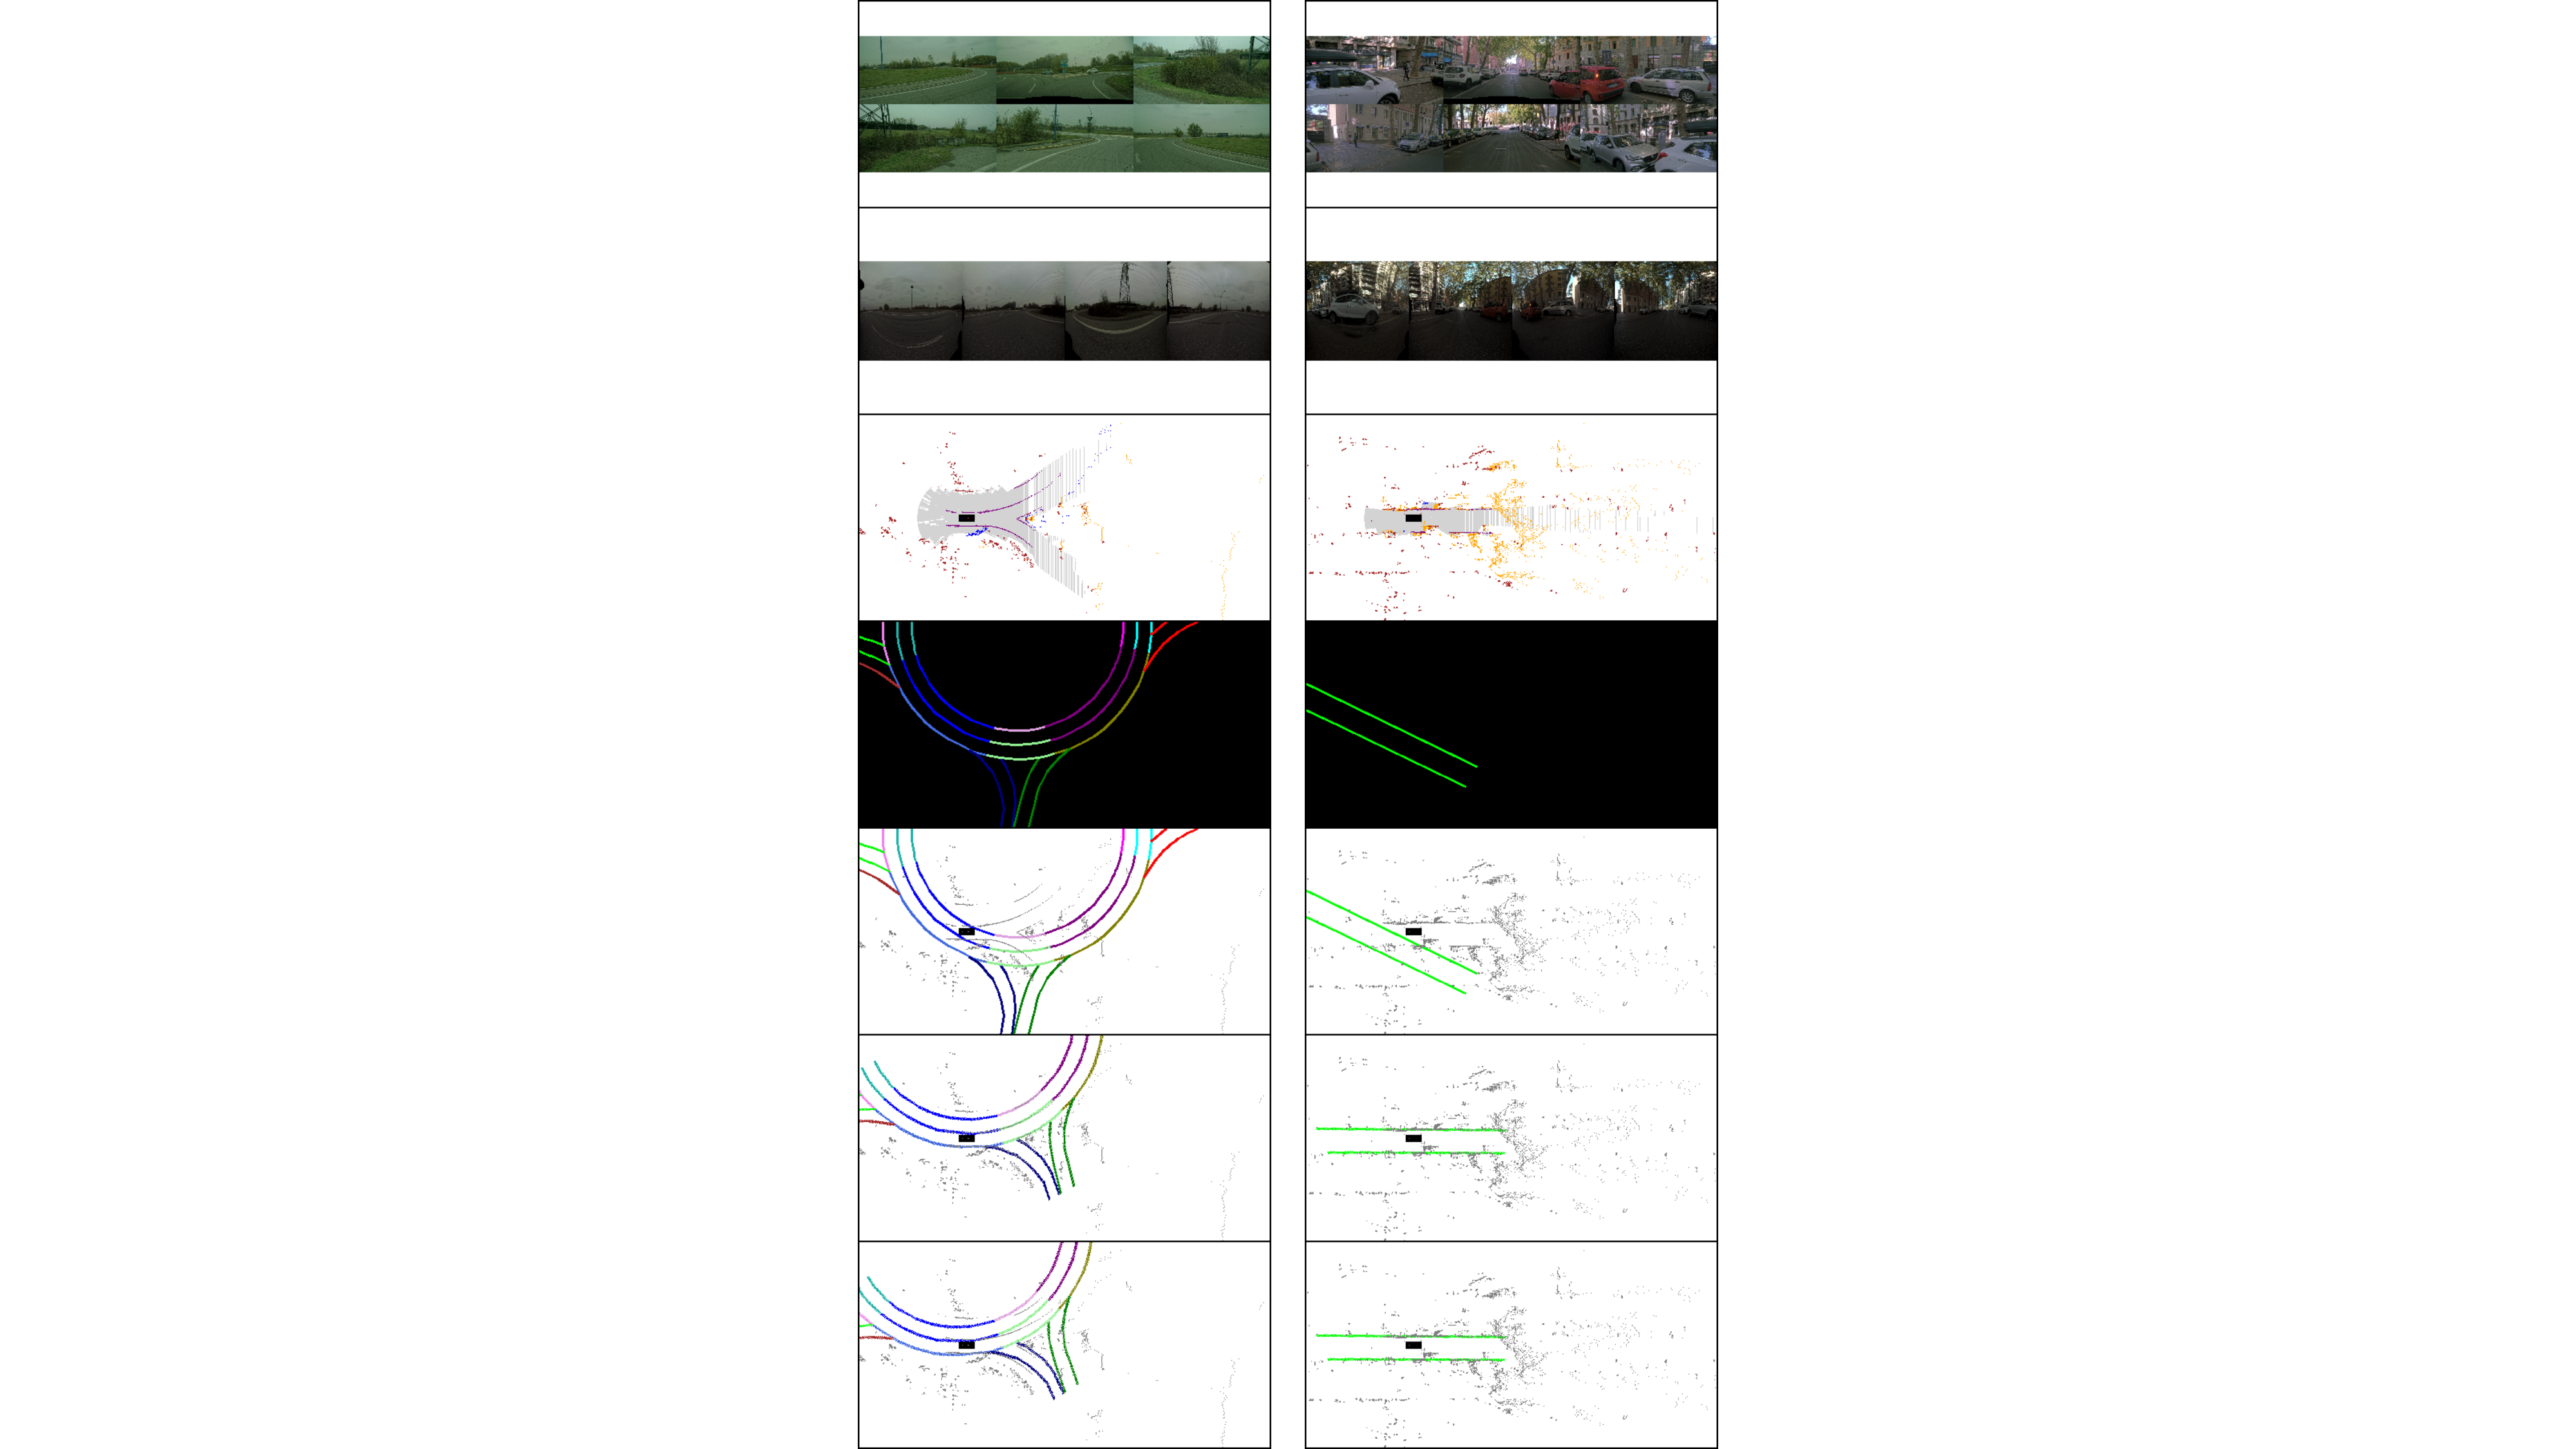
\includegraphics[width=0.8\linewidth]{LateX//figs/bev_traininig_phases.pdf}
    \caption{Training progression during early and advanced phases, showing input images from long-range and short-range cameras.}
    \label{fig:bev_training_phases}
\end{figure}

The results of the evaluation, as presented in Table~\ref{tab:pose_variations}, indicate significant improvements compared to the previous approach. The high precision achieved in alignment suggests that the proposed method can perform at a level comparable to, or even exceeding, state-of-the-art techniques. However, direct comparisons with state-of-the-art methods are challenging, as the tests were conducted on different datasets, which could influence overall performance metrics.

\begin{table}[H]
    \centering
    \scriptsize
    \begin{tabular}{>{\centering\arraybackslash}p{2.25cm} >{\centering\arraybackslash}p{2.25cm} >{\centering\arraybackslash}p{3.25cm} >{\centering\arraybackslash}p{2.25cm} >{\centering\arraybackslash}p{2.25cm}}
        \toprule
        \textbf{Iteration} & \textbf{$\Delta$ Pose} & \textbf{$\Delta \theta$} & \textbf{$\Delta x + \Delta y$} & \textbf{$\Delta h$} \\
        & \text{[m]} & \text{[deg]} & \text{[m]} & \text{[m]} \\
        \midrule
        \num{20000} & 0.52 & 1.4  & 0.50 & 0.01 \\
        \num{40000} & 0.32 & 0.6  & 0.31 & 0.00 \\
        \num{60000} & 0.08 & 0.12  & 0.08 & 0.00\\
        \num{80000} & 0.05 & 0.01  & 0.05 & 0.00 \\
        \num{100000} & \textbf{0.01} & \textbf{0.004} & \textbf{0.01} & \textbf{ 0.00} \\
        \bottomrule
    \end{tabular}
    \caption{Evaluation (L1) values in pose, angle, combined displacement ($\Delta x + \Delta y$), and height across iterations using Smooth L1 Loss Function, SGD,  and BEV reconstruction.}
    \label{tab:pose_variations}
\end{table}

Figures~\ref{fig:loss_comparison_2} and~\ref{fig:total_loss_2} illustrate the loss progression during training. The observed behavior, with the loss steadily decreasing despite minor noise, suggests stable training dynamics without divergence. The evaluation results further confirm that \textit{overfitting} was avoided, as the model generalizes well to unseen data.
\begin{figure}[H]
    \centering
    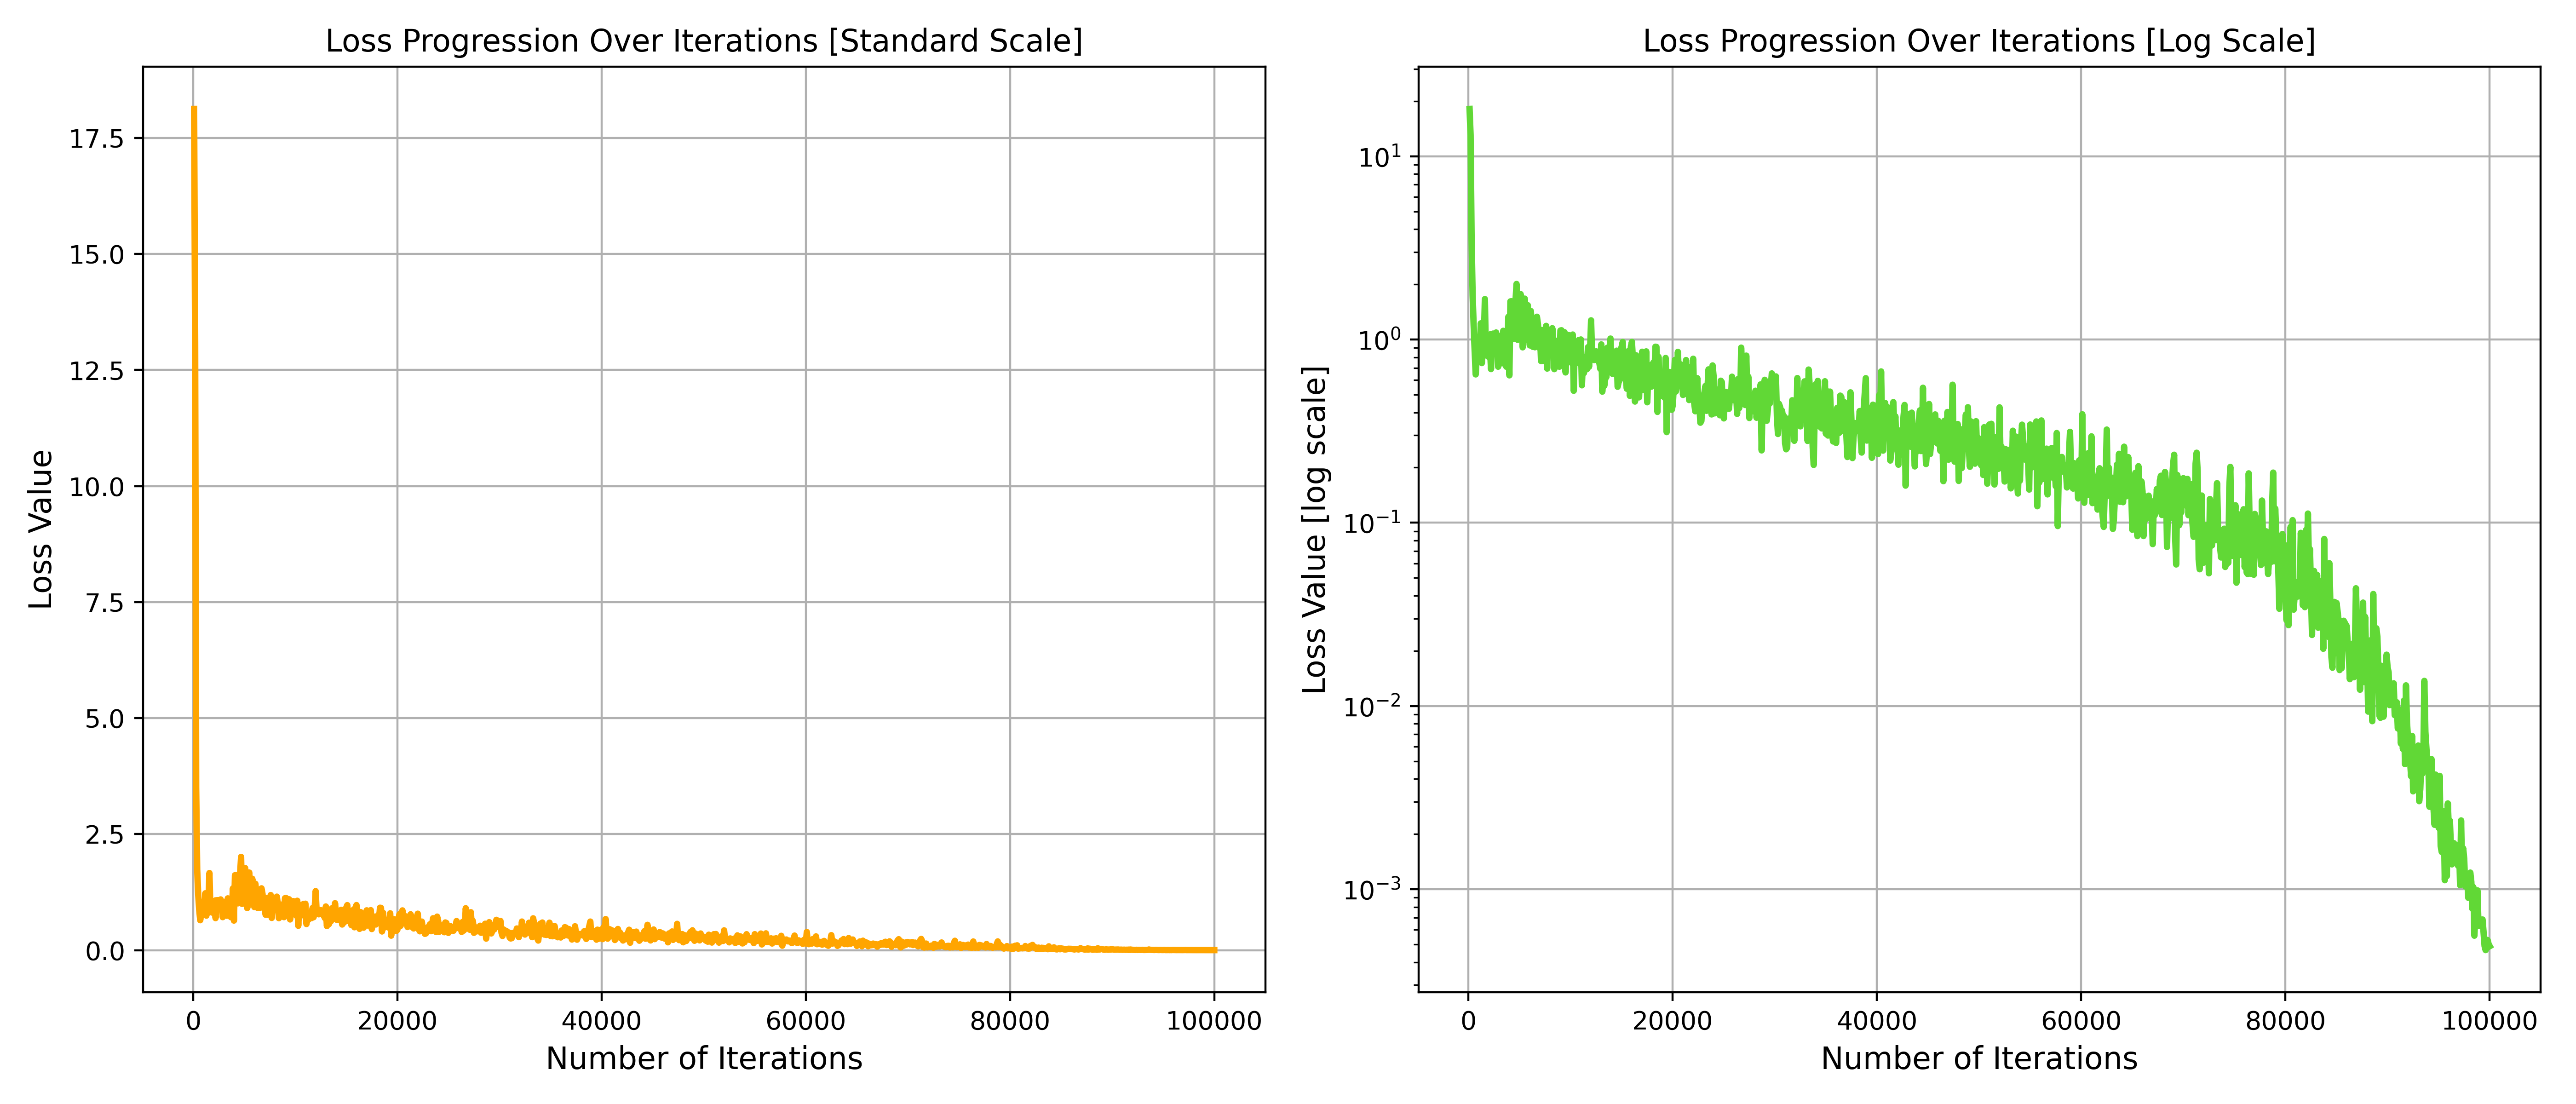
\includegraphics[width=1\linewidth]{LateX//figs/BEV2_loss_total_l1sDEG_progression_comparison.png}
    \caption{Total loss progression using the Smooth L1 Loss, SGD and BEV reconstruction. The plot includes a standard scale (left) and logarithmic scale (right).}
    \label{fig:loss_comparison_2}
\end{figure}
\begin{figure}[H]
    \centering
    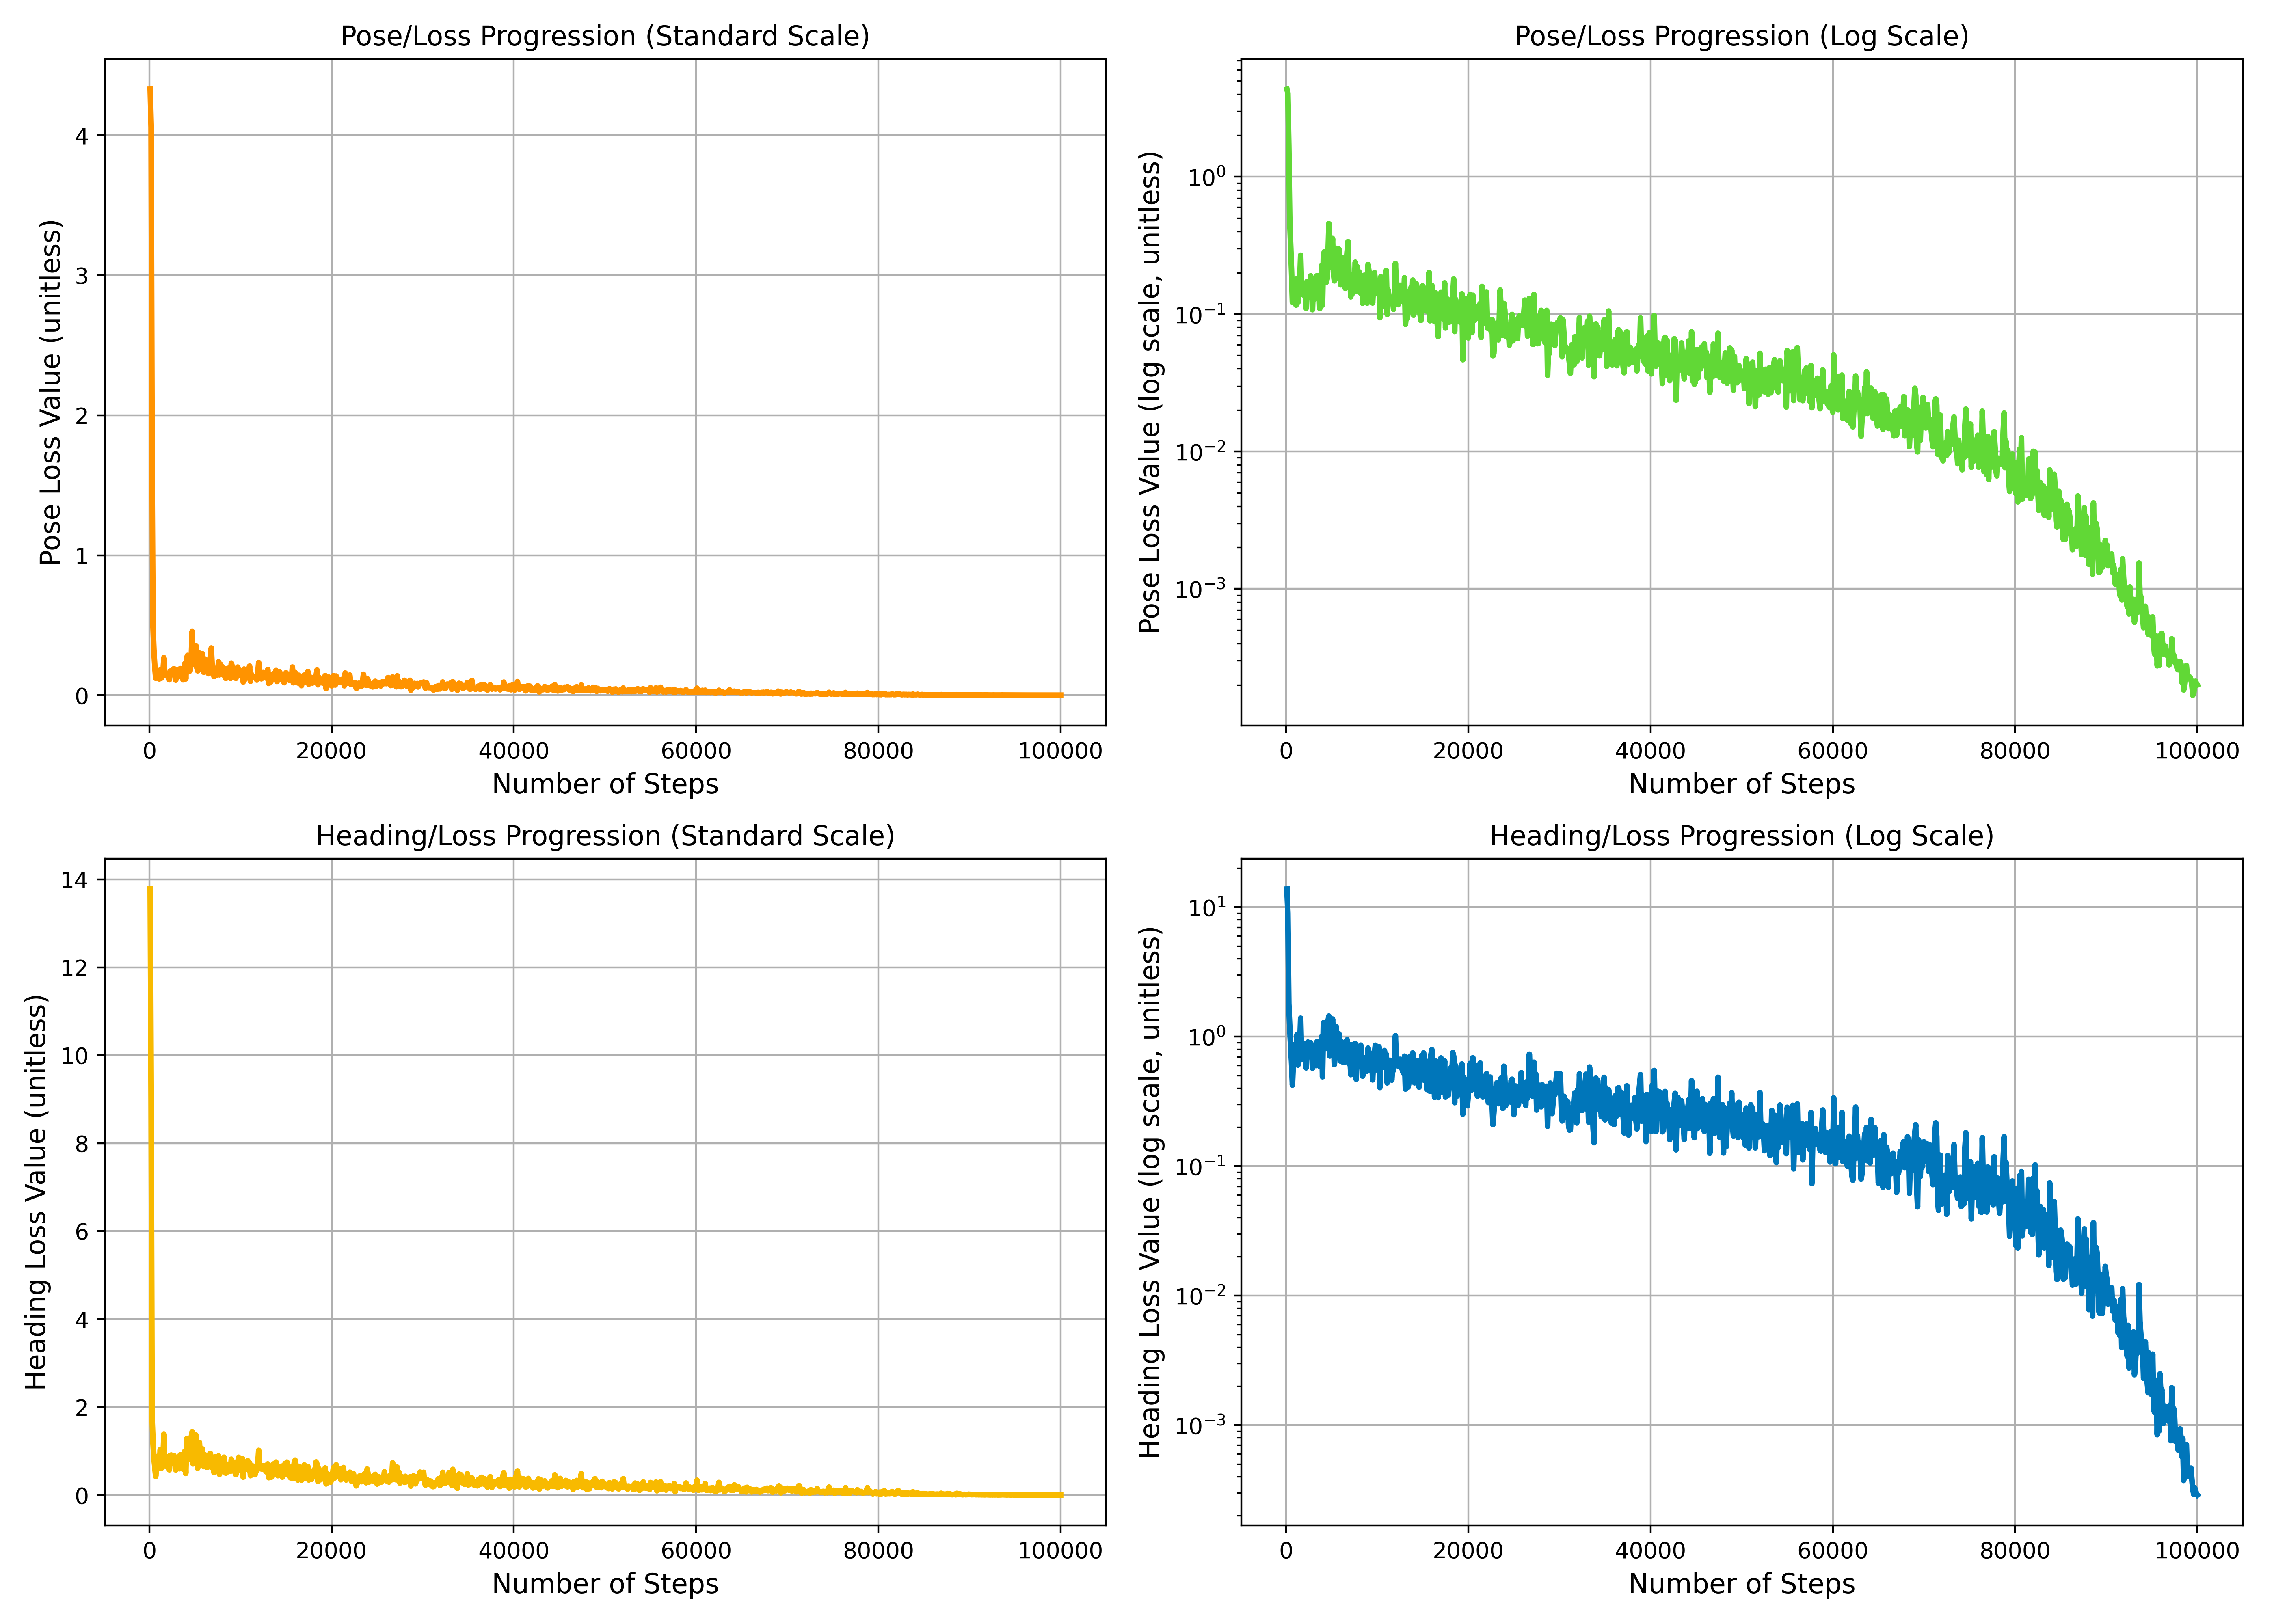
\includegraphics[width=1\linewidth]{LateX//figs/BEV2_l1sDEG_pose_heading_loss_comparison.png}
    \caption{Pose (orange) and Heading (yellow) Loss comparison during training. The plot includes a standard scale on the left and a logarithmic scale on the right.}
    \label{fig:total_loss_2}
\end{figure}

\subsection*{Adam Optimizer}

An attempt was made to use the Adam optimizer for training. Adam typically requires a much lower learning rate compared to SGD to achieve similar performance, as commonly discussed in literature. 
\begin{figure}[H]
    \centering
    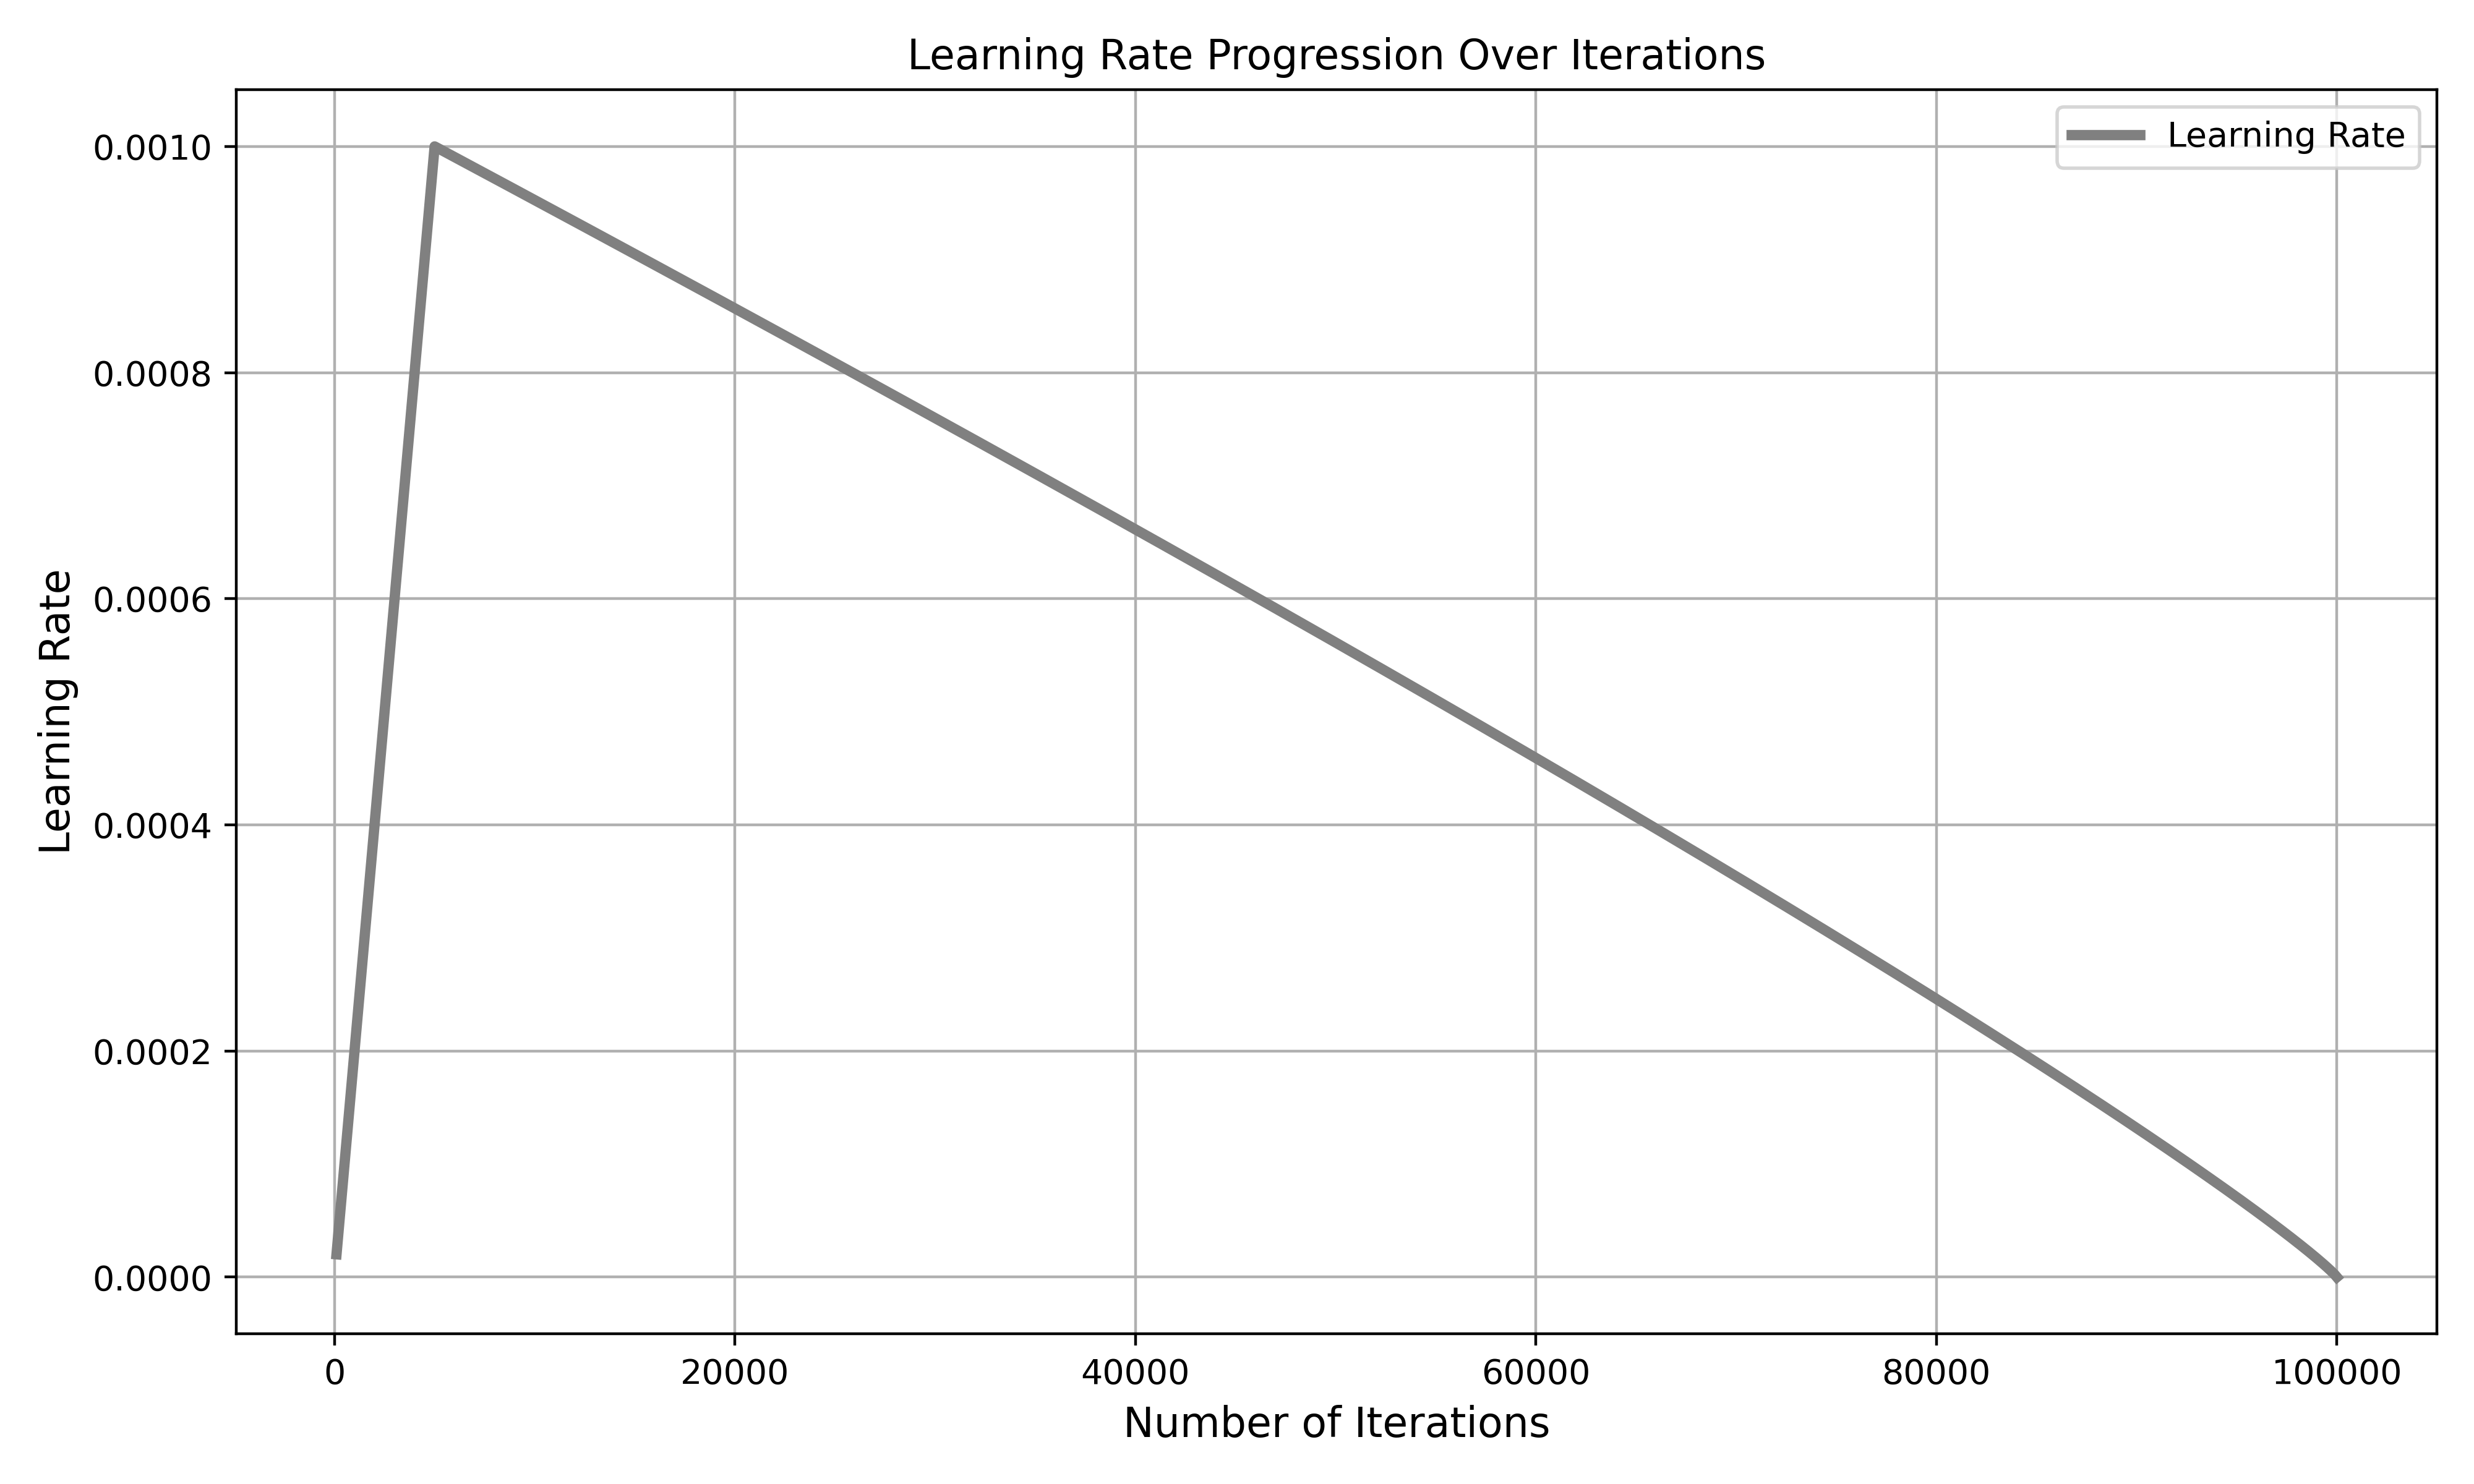
\includegraphics[width=0.75\linewidth]{BEV2learning_rate_progression.png}
    \caption{Learning rate progression during training with Adam, showcasing an initial warm-up phase followed by a gradual decrease. The learning rate peaks at a maximum value of $0.001$ at $5000$ iterations.}
    \label{fig:adam_learning_rate}
\end{figure}

Adam is a popular optimization algorithm in deep learning that combines the advantages of both the AdaGrad and RMSProp algorithms. It computes adaptive learning rates for each parameter by maintaining running averages of the gradients (momentum) and their squared values. This approach guarantees fast convergence and robustness in handling sparse gradients, making Adam well-suited for tasks with noisy or complex datasets.

The loss curves observed during training with Adam showed consistent downward trends, as expected, indicating stable learning. Evaluating the results in Table~\ref{tab:pose_variations_1} further supports the conclusion that the model did not \textit{overfit}, maintaining good generalization capabilities. 

\begin{figure}
    \centering
    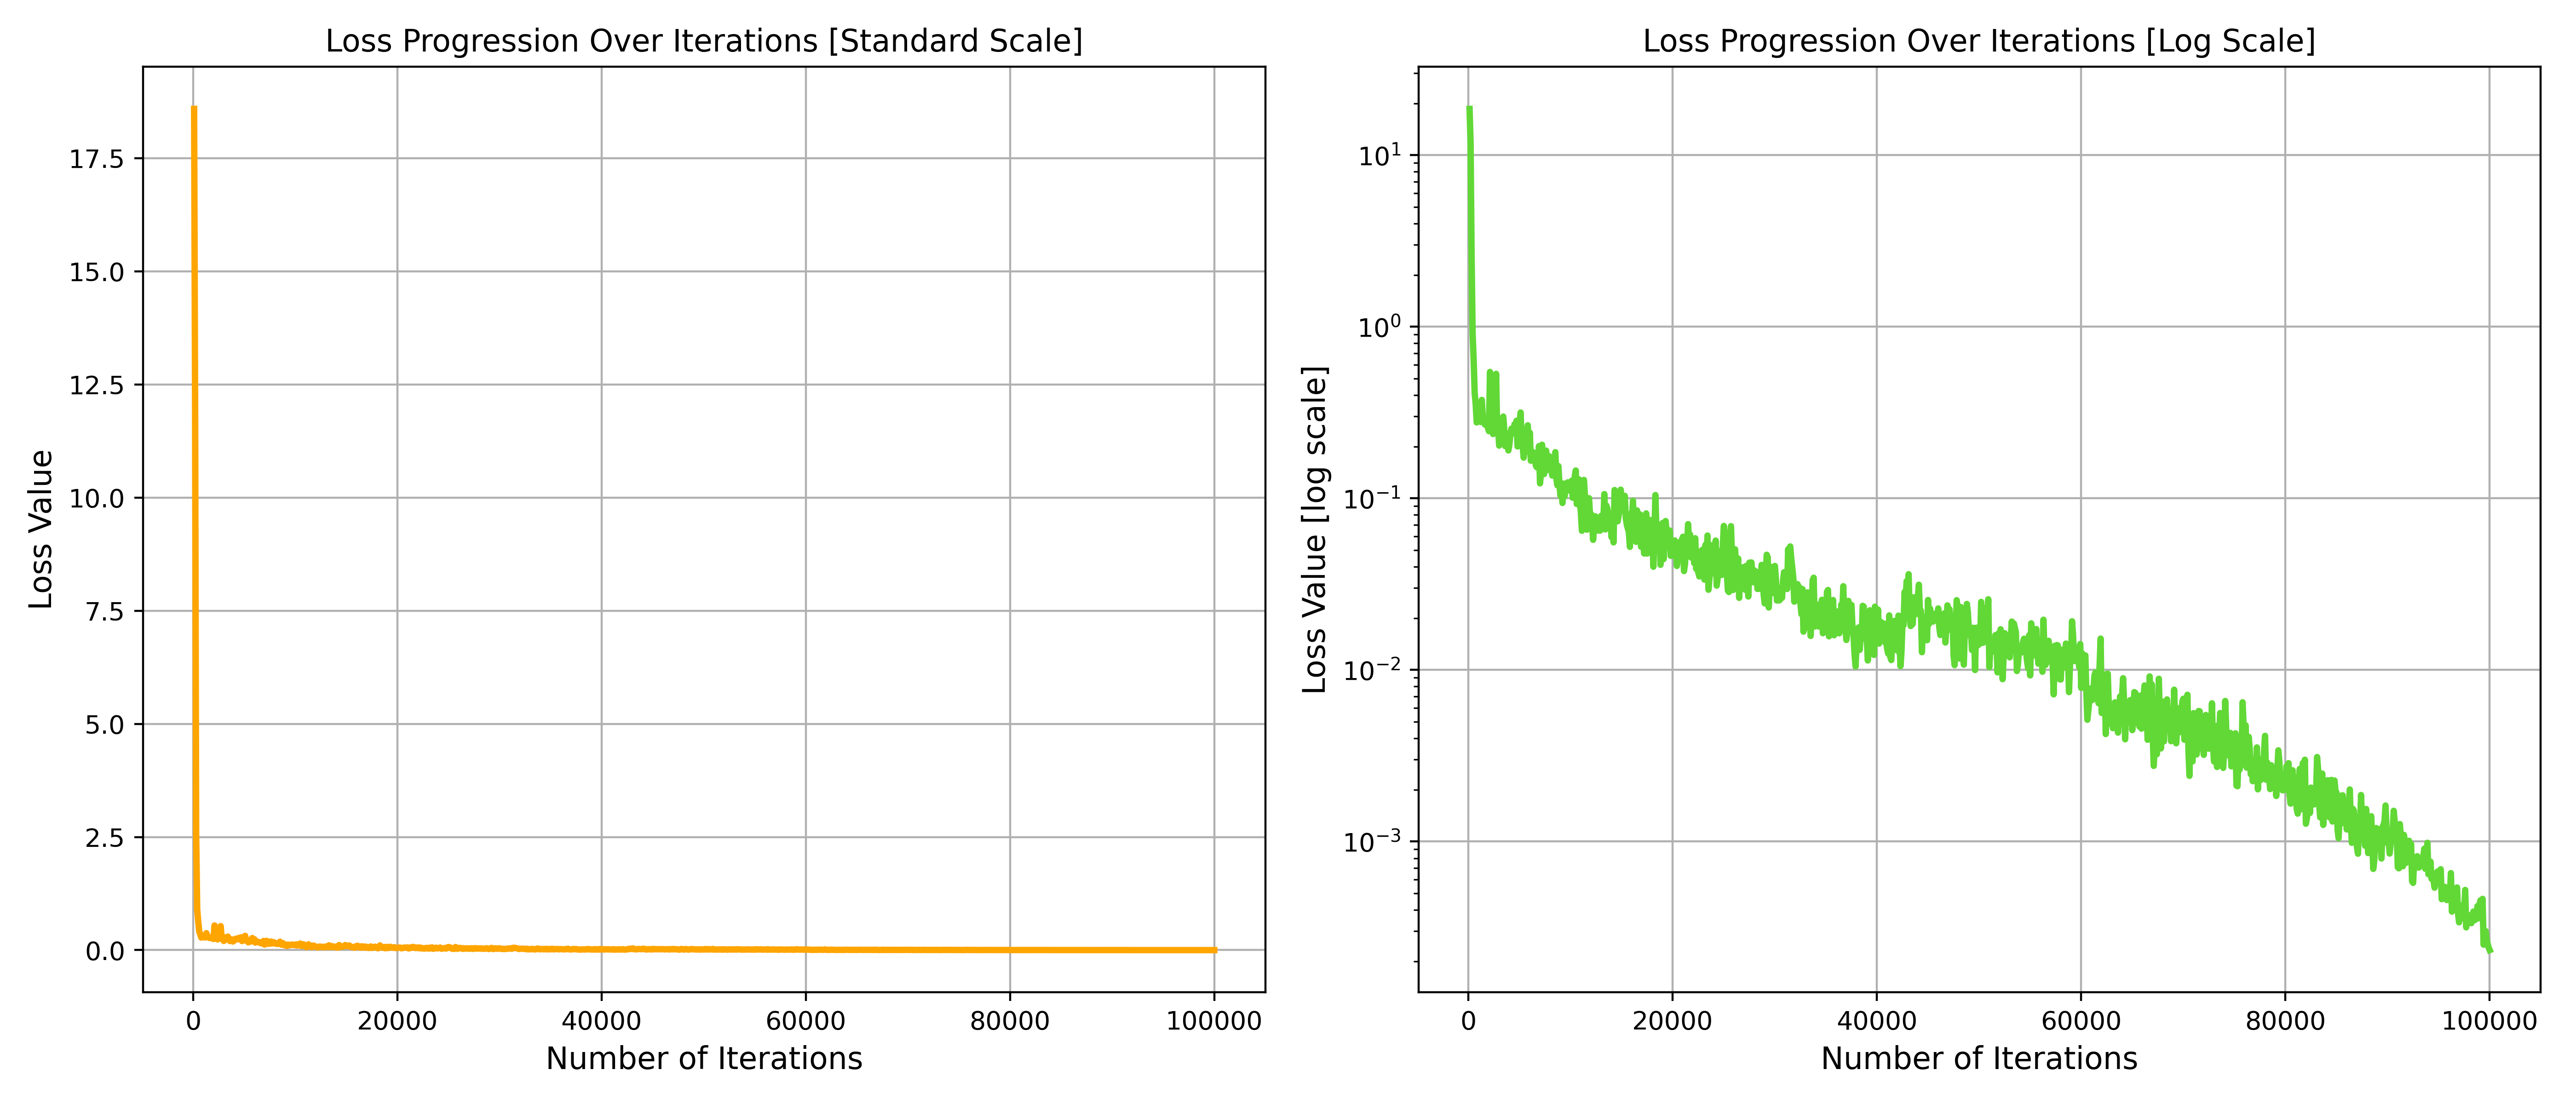
\includegraphics[width=1\linewidth]{LateX//figs/BEV1_loss_total_l1sDEG_progression_comparison.png}
    \caption{Total loss progression using the Smooth L1 Loss, Adam and BEV reconstruction. The plot includes a standard scale (left) and logarithmic scale (right).}
    \label{fig:adam_loss_progression}
\end{figure}

Despite these promising results, the performance appeared to plateau toward the end of the training. It is likely that better results could have been achieved by extending the training for a few more iterations, potentially up to 10\% more, to allow further fine-tuning and refinement of the learned features.

\begin{figure}
    \centering
    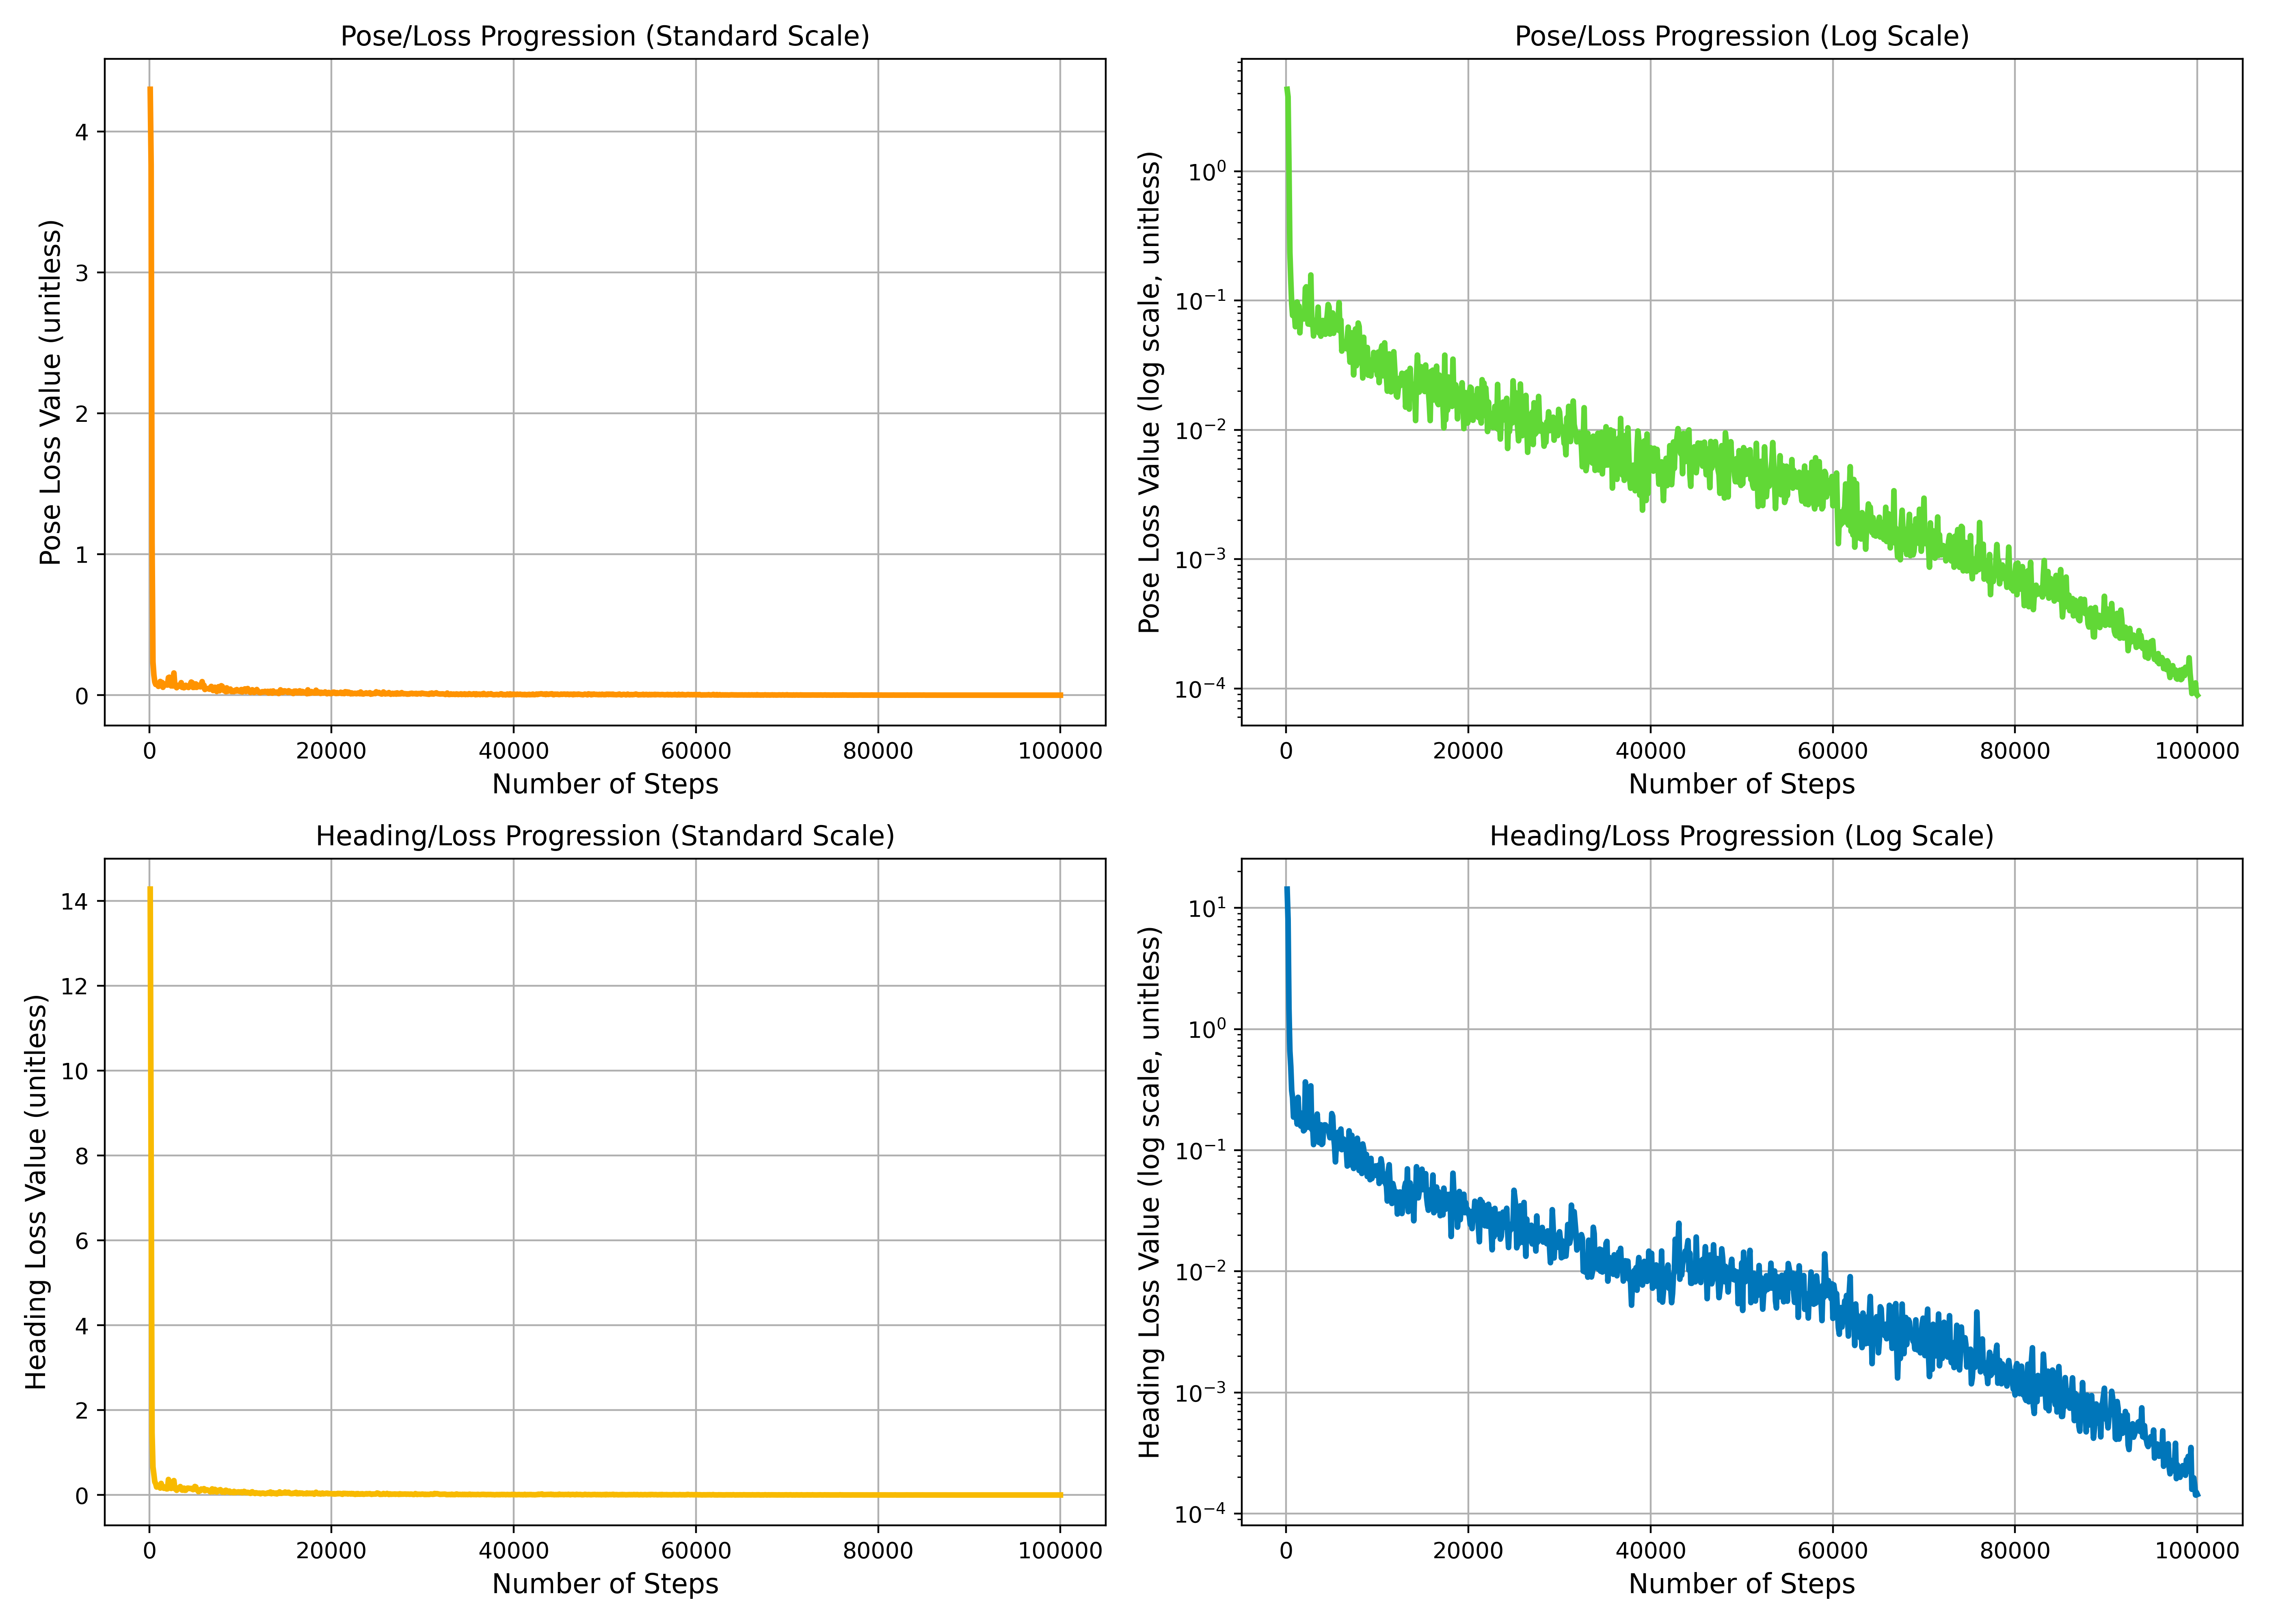
\includegraphics[width=1\linewidth]{LateX//figs/BEV1_l1sDEG_pose_heading_loss_comparison.png}
    \caption{Pose (orange) and Heading (yellow) Loss comparison during training. The plot includes a standard scale on the left and a logarithmic scale on the right.}
    \label{fig:adam_loss_comparison}
\end{figure}

The choice of optimizer is a recurring topic in machine learning research. It is often argued that while Adam converges faster, SGD tends to generalize better, leading to improved final performance. This distinction is supported by studies such as \cite{DBLP:journals/corr/abs-1910-05446}, which suggest that minimizing training time can reduce the risk of \textit{overfitting}. A shorter training duration limits the number of times the model sees the same data, thus preserving generalization capability. This behavior was also observed during training with Adam, as reflected in the loss functions and evaluation results.

\begin{table}[H]
    \centering
    \scriptsize
    \begin{tabular}{>{\centering\arraybackslash}p{2.25cm} >{\centering\arraybackslash}p{2.25cm} >{\centering\arraybackslash}p{3.25cm} >{\centering\arraybackslash}p{2.25cm} >{\centering\arraybackslash}p{2.25cm}}
        \toprule
        \textbf{Iteration} & \textbf{$\Delta$ Pose} & \textbf{$\Delta \theta$} & \textbf{$\Delta x + \Delta y$} & \textbf{$\Delta h$} \\
        & \text{[m]} & \text{[deg]} & \text{[m]} & \text{[m]} \\
        \midrule
        \num{20000}  & 0.58 & 1.50   & 0.57 & 0.01 \\
        \num{40000}  & 0.41 & 0.90   & 0.41 & 0.00 \\
        \num{60000}  & 0.10 & 0.23  & 0.10 & 0.00 \\
        \num{80000}  & 0.07 & 0.01  & 0.07 & 0.00 \\
        \num{100000} & \textbf{0.03} & \textbf{0.004} & \textbf{0.03} & \textbf{ 0.00} \\
        \bottomrule
    \end{tabular}
    \caption{Evaluation (L1) values in pose, angle, combined displacement ($\Delta x + \Delta y$), and height across iterations using Smooth L1 Loss Function, Adam, and BEV reconstruction.}
    \label{tab:pose_variations_1}
\end{table}

Adam appears to be an excellent choice when the goal is to accelerate training, but it may not be ideal for achieving the lowest local minima or the highest possible performance. Its faster convergence makes it a practical option for iterative experimentation or when computational resources are limited, but SGD remains more suitable for fine-tuning models to achieve optimal generalization and final performance.

\subsection{Inference}

As in the initial approach, the model was tested by performing inference on sequences that were not included during the training phase. Figure~\ref{fig:bev_inference_2} highlights three particularly interesting scenarios, demonstrating the model's robustness in diverse and challenging conditions.

In the first case, the model performs well even on a straight road with minimal texture, a condition that previously posed difficulties for alignment. This result underscores the improved capability of the model to handle scenarios with limited visual cues.

The second example involves a complex situation: an intersection with multiple lanes that gradually disappear shortly after the crossing. Despite the intricate nature of this environment, the model successfully maintains alignment, demonstrating its abilities.

The third case is not common. The vehicle is not situated within a specific lane but is in a merging phase, positioned between two lanes. Even in this challenging configuration, the model achieves a highly accurate alignment, highlighting its adaptability to unconventional driving scenarios.

Across these examples, and in the majority of cases not explicitly shown here, the model consistently exhibits strong performance, achieving reliable alignment under varying and sometimes extreme conditions.
\begin{figure}[H]
    \centering
    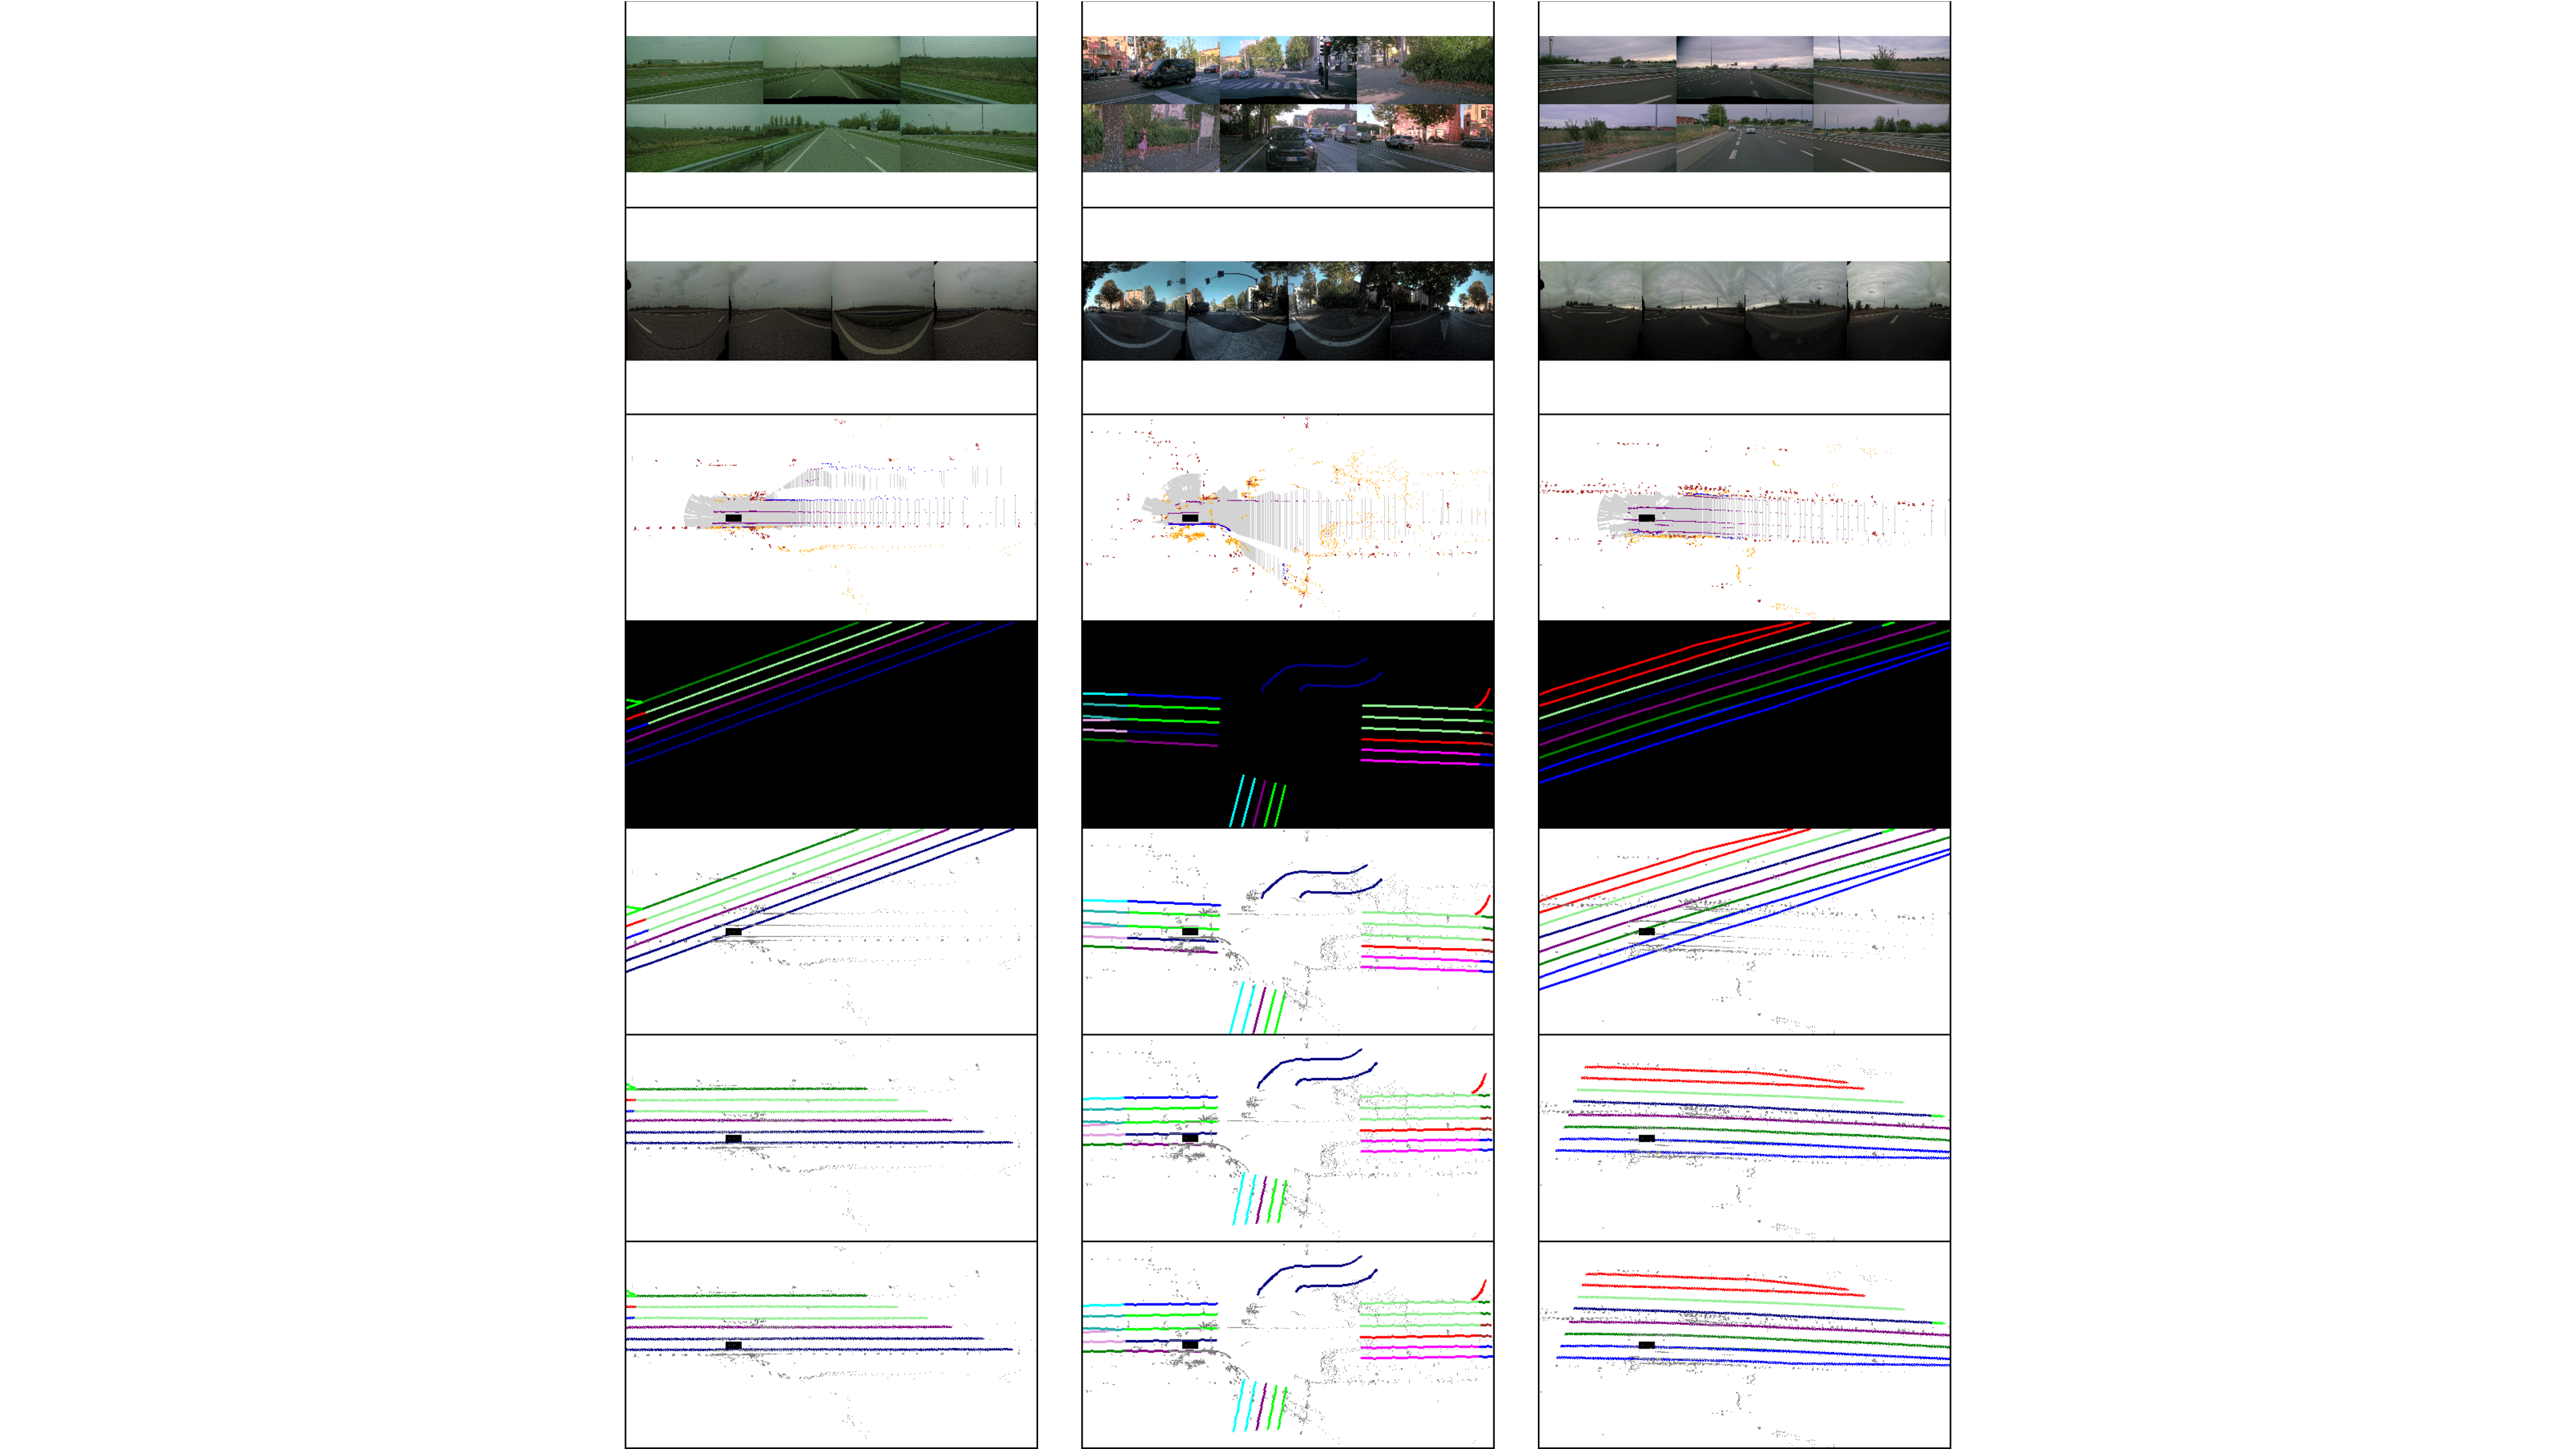
\includegraphics[width=1\linewidth]{LateX//figs/bev_inference.pdf}
    \caption{Examples of inference results in different scenarios: minimal texture, complex intersections, and lane merging.}
    \label{fig:bev_inference_2}
\end{figure}